\documentclass[master, fontsize=14]{diploma}

% Дополнительные математические символы (\varnothing, \mathbb, \setminus и т.п.).
\usepackage{amssymb}

% Горизонтальные линейки в таблицах (\toprule, \midrule, \bottomrule).
\usepackage{booktabs}

\hyphenation{
  не-струк-ту-ри-ро-ван-но-го
  цент-ра-ли-зо-ван-ное
  ав-то-ма-ти-чес-кое
  мно-го-уров-не-вой
  чувст-ви-тель-ная
  до-ми-ни-ру-ю-щая
  про-из-водст-вен-ный
  стра-ти-фи-ци-ро-ван-ной
  тру-до-ём-кость
}

% Общая media-library в корне репо: используется и report, и slides.
\graphicspath{{../images/}}

\student{Фролов Михаил Александрович}
\group{М8О-206СВ-24}
\theme{Система автоматизированного обогащения товарных данных для интернет-магазина}

\supervisor{Судаков Владимир Анатольевич}

\faculty{№ 8 «Компьютерные науки и прикладная математика»}
\department{Института №8}
\speciality{01.04.02 Прикладная математика и информатика}
\profile{Продуктовая разработка и разработка программных систем}

\departmentFullName{№ 806 <<Вычислительная математика и программирование>>}
\headOfDepartment{Крылов Сергей Сергеевич}

% Дата. Оставляем пустое место для дня.
\date{\uline{\hspace{20pt}}~\uline{\hspace{60pt}}~20\uline{\hspace{20pt}}~г.}

% Сокращения и обозначения (\listofabbreviations подтягивает их по \newacronym).
% Порядок — по алфавиту (латиница, затем кириллица), как требует ГОСТ 7.32.
\newacronym{aop}{AOP}{Appellation d'Origine Prot\'eg\'ee, защищённое наименование места происхождения (фр., эквивалент PDO)}
\newacronym{api}{API}{application programming interface, программный интерфейс приложения}
\newacronym{bic}{BIC}{Bayesian Information Criterion, байесовский информационный критерий выбора структуры сети}
\newacronym{ci}{CI}{confidence interval, доверительный интервал (95\,\% если не указано иное)}
\newacronym{e2e}{E2E}{end-to-end (сквозной); сквозная точность системы с учётом маршрутизации и отказа от ответа (отказ засчитывается как ошибка); производственно-реалистичная метрика, см. термин «Сквозная точность»}
\newacronym{ece}{ECE}{Expected Calibration Error, ожидаемая ошибка калибровки вероятностей классификатора}
\newacronym{json}{JSON}{JavaScript Object Notation, текстовый формат обмена данными}
\newacronym{lightgbm}{LightGBM}{Light Gradient Boosting Machine, библиотека градиентного бустинга деревьев решений}
\newacronym{llm}{LLM}{large language model, большая языковая модель}
\newacronym{ml}{ML}{machine learning, машинное обучение}
\newacronym{mlp}{MLP}{multi-layer perceptron, многослойный персептрон (полносвязная нейронная сеть)}
\newacronym{mpnet}{MPNet}{Masked and Permuted Pre-training, архитектура трансформера, использованная в paraphrase-multilingual-mpnet-base-v2 для 768-мерных векторных представлений}
\newacronym{odbl}{ODbL}{Open Database License v1.0, лицензия с наследованием (share-alike) для открытых баз данных; применяется к Open Food Facts}
\newacronym{off}{OFF}{Open Food Facts, открытый краудсорсинговый каталог продовольственных товаров под лицензией ODbL}
\newacronym{ood}{OOD}{out-of-distribution, выход за пределы обучающего распределения}
\newacronym{pdo}{PDO}{Protected Designation of Origin, защищённое наименование места происхождения}
\newacronym{pim}{PIM}{product information management, управление информацией о товарах}
\newacronym{rest}{REST}{representational state transfer, архитектурный стиль программного интерфейса}
\newacronym{sbert}{SBERT}{Sentence-BERT, многоязычная модель векторного представления предложений}
\newacronym{sku}{SKU}{stock keeping unit, товарная учётная позиция (артикул)}
\newacronym{tfidf}{TF-IDF}{term frequency $\times$ inverse document frequency, частота терма, взвешенная обратной частотой документа (мера значимости слова в корпусе)}
\newacronym{xgb}{XGBoost}{Extreme Gradient Boosting, библиотека градиентного бустинга деревьев решений}
\newacronym{tz}{ТЗ}{техническое задание}

% Определения терминов (\termsanddefenitions подтягивает их по \newglossaryentry).
\newglossaryentry{silver_labels}{
    name={Серебряная разметка},
    description={набор пар «товар --- целевое значение атрибута», полученный автоматически из открытых источников данных (теги Open Food Facts, OFF) и используемый для обучения моделей. Содержит шум и неполноту; противопоставляется эталонной разметке}
}
\newglossaryentry{gold_labels}{
    name={Эталонная разметка},
    description={пары «товар --- целевое значение», прошедшие верификацию согласованным мнением нескольких больших языковых моделей и (или) слепой разметкой более сильной модели; используется как опорная истина при оценке каскада}
}
\newglossaryentry{weak_supervision}{
    name={Обучение со слабой разметкой (англ.\ weak supervision)},
    description={режим обучения с использованием неполной или зашумлённой разметки, формируемой автоматически из доступных источников вместо ручной разметки экспертом}
}
\newglossaryentry{cascade_arch}{
    name={Каскадная архитектура},
    description={последовательность алгоритмических слоёв, каждый из которых обрабатывает только те ячейки «товар, атрибут», которые не были закрыты предыдущими слоями выше калиброванного порога уверенности}
}
\newglossaryentry{router_term}{
    name={Маршрутизатор (категорий)},
    description={предкаскадный классификатор-распределитель (Слой 0): по партнёр-доступным полям определяет товарную категорию либо относит товар к классу вне области охвата (OOD), после чего запускается схема каскада соответствующей категории}
}
\newglossaryentry{conf_filter}{
    name={Пошаговая фильтрация по уверенности},
    description={формализация поведения каскада как последовательного конъюнктивного условия на прохождение калиброванных порогов уверенности на каждом слое каскада}
}
\newglossaryentry{coverage}{
    name={Покрытие},
    description={доля ячеек «товар, атрибут» в тестовой выборке, для которых каскад дал предсказание выше порога уверенности на слоях 1--3 (без обращения к запасному слою)}
}
\newglossaryentry{covered_acc}{
    name={Точность на покрытом срезе},
    description={доля верных предсказаний среди тех ячеек, для которых каскад дал ответ без обращения к запасному слою}
}
\newglossaryentry{end2end_acc}{
    name={Сквозная точность},
    description={точность системы на полной тестовой выборке, при которой отказы каскада засчитываются как неверные ответы (либо заменяются ответом запасного слоя при включённом Слое 4)}
}
\newglossaryentry{code_disjoint}{
    name={Разбиение без пересечения товарных кодов},
    description={деление выборки на обучающую и тестовую части так, что ни один товарный код (баркод) не попадает одновременно в обе части; обеспечивает оценку качества системы на новых товарных позициях}
}
\newglossaryentry{audit_loop}{
    name={Цикл «аудит --- правки --- переобучение --- измерение»},
    description={методология итеративного улучшения системы: выявленные при аудите дефекты эталонной разметки устраняются правкой экстрактора признаков, после чего модели переобучаются, а прирост точности измеряется на той же контрольной выборке}
}


\addbibresource{main.bib}

\begin{document}
    \maketitle

    % \includepdf[pages=-]{extra/task} % Задание (оформляется отдельно).
    \setcounter{page}{2}

    \abstract
\keywords{ОБОГАЩЕНИЕ ТОВАРНЫХ ДАННЫХ, КАСКАДНАЯ АРХИТЕКТУРА, СЛАБЫЙ НАДЗОР, OPEN FOOD FACTS, БАЙЕСОВСКАЯ СЕТЬ, БОЛЬШАЯ ЯЗЫКОВАЯ МОДЕЛЬ, КАЛИБРОВКА, ИЗВЛЕЧЕНИЕ ПРИЗНАКОВ, ДОМИНИРОВАНИЕ ПО ПАРЕТО, АУДИТ-ЦИКЛ, ВЕКТОРНЫЕ ПРЕДСТАВЛЕНИЯ}

\textbf{Объём работы.} 91 страница основной части, 4 главы, 9 рисунков, 22 таблицы, 52 источника (16 российских и 36 зарубежных).

\textbf{Объект исследования.} Процесс автоматизированного обогащения товарных каталогов интернет-магазинов с использованием открытых источников данных.

\textbf{Предмет исследования.} Гибридная каскадная архитектура с ансамблевой оценкой уверенности классификаторов и адаптивным обращением к большой языковой модели как запасному слою.

\textbf{Цель работы.} Разработать гибридную каскадную систему автоматизированного обогащения товарных данных для интернет-магазина, обеспечивающую высокую точность извлечения категориальных атрибутов при сокращённой стоимости обращения к большой языковой модели и поддерживающую развёртывание на открытых моделях.

\textbf{Методы.} Многоязычные векторные представления текста на базе модели paraphrase-multilingual-MiniLM-L12-v2 (SBERT, поддержка 50+ языков), классификатор XGBoost с регуляризацией и поатрибутными порогами уверенности, байесовская сеть со структурой, найденной алгоритмом Hill Climb по критерию BIC (библиотека pgmpy), доверительные интервалы с кластеризацией по брендам через ресэмплированный бутстрэп, бакетирование числовых нутри-полей, согласие трёх независимых больших языковых моделей (Sonnet 4.5 + GPT-4o + Gemini 2.5 Flash) для построения эталонной разметки на текстово-семантических атрибутах, слепая верификация моделью Claude Opus 4, разбиение на обучающую и тестовую части без пересечения товарных кодов (code-disjoint), проверка гипотезы, зафиксированной до получения результатов с поправкой Бонферрони на множественные сравнения.

\textbf{Результаты.} Реализована и эмпирически проверена гибридная каскадная архитектура из пяти слоёв (категорайзер Слой 0 — регулярные выражения — классификатор XGBoost на векторных представлениях SBERT — байесовский валидатор плотностей — запасной слой большой языковой модели) на трёх продуктовых категориях открытого каталога Open Food Facts (паста, шоколад, сыры). На тестовой выборке без пересечения товарных кодов (code-disjoint, новые SKU) размером 3257 ячеек по 20 парам «категория-атрибут» итоговая конфигурация достигает 91,1 \% сквозной точности при обращении к большой языковой модели на 7,1 \% ячеек в режиме «каскад + gemini-flash»; точность только-каскадной части (без учёта непокрытых ячеек) составляет 94,8 \% (macro-F1 0,899). На консервативной нижней оценке с независимой экспертной разметкой моделью Claude Opus 4 (n=615) — 87,5 \% сквозной точности. При развёртывании на собственных мощностях с открытой моделью gpt-oss-120b — 90,6 \% точности, что на 21,3 п. п. выше прямого использования gpt-oss-120b (69,3 \%). Каскад без запасного слоя покрывает 96,0 \% ячеек. Достигнуто доминирование по Парето разработанной системы над прямым использованием большой языковой модели по двум осям одновременно — точности и стоимости (+7,3 п. п. точности и сокращение стоимости в 333 раза при той же экономии по сравнению с прямым использованием Claude Sonnet 4.5; архитектурное сокращение стоимости в 14 раз обеспечивается переводом 92,9 \% ячеек на дешёвые слои каскада). Гипотеза, зафиксированная до получения результатов, о превосходстве обучаемого стоимостно-чувствительного маршрутизатора над статическим правилом отклонена после поправки Бонферрони на трёх бюджетах. Реализован замкнутый цикл «аудит — правки экстрактора — переобучение — измерение» с кросс-категорийной репликацией 3 из 3. Разработана демонстрационная система из трёх компонентов (шлюз API на Go, ML-сервис на Python/FastAPI, веб-интерфейс), реализующая стабильный контракт REST API.

\textbf{Использование результатов.} Разработанная архитектура применима в системах управления товарной информацией (PIM-системах) интернет-магазинов. Внедрение системы позволяет: повысить полноту автоматического заполнения карточек товаров до 91,1 \% (сквозная точность с учётом маршрутизации; 94,8 \% по каскадной части как верхняя граница при идеальной маршрутизации категории), сократить стоимость обработки в 333 раза по сравнению с прямым использованием Claude Sonnet 4.5 (комбинированное сокращение, включающее архитектурный вклад каскада в 14 раз и удешевление модели запасного слоя), сократить ручную нагрузку оператора каталога в 10–14 раз за счёт перевода в режим выборочной верификации, обеспечить развёртывание на собственных мощностях без отправки партнёрских данных во внешние API больших языковых моделей.

      % Реферат

    \tableofcontents                   % Содержание
    \termsanddefenitions               % Термины и определения
    \listofabbreviations               % Перечень сокращений и обозначений

    \introduction

\paragraph*{Актуальность темы исследования.}

Электронная коммерция продолжает расти. Годовой объём российского сегмента в 2025 году составил 11,5~трлн~руб. \cite{ref_1}, мировой рынок тоже показывает рост \cite{ref_2}. Каталоги крупных интернет-магазинов содержат десятки миллионов товарных позиций: только индексируемая часть каталога Ozon в открытых аналитических базах превышает 38~млн позиций \cite{ref_3}. Ежедневно туда добавляются тысячи новых записей от партнёров-поставщиков.

Карточка товара — центральный элемент цифровой витрины. От её полноты зависят фасетный поиск, релевантность ранжирования и рекомендаций, корректность аналитики и в итоге конверсия в покупки. Партнёрский ввод при этом неоднородный: для одного товара поставщик передаёт только название и бренд, для другого — расширенный набор полей с фотографиями, для третьего — состав на иностранном языке. Образующиеся пробелы исторически закрывают контент-менеджеры вручную: каждую карточку приходится открывать, проверять и дописывать десятки атрибутов. На каталоге в миллионы позиций и тысячах новых записей в сутки это уже не работает ни по затратам, ни по доступности знаний иностранных языков \cite{ref_4}.

Системы управления товарной информацией (Product Information Management) — Akeneo, Pimcore, Salsify и аналогичные \cite{ref_5, ref_6, ref_7} — сложились из задачи хранить уже сформированную товарную информацию. Задачу извлечения этой информации из неструктурированного партнёрского ввода они системно не решают. Появляющиеся в них модули автоматического обогащения — это, как правило, обёртка над одной публичной большой языковой моделью с прямым вызовом на каждый товар. Подробное сопоставление приведено в~\ref{subsubsec:analogs}. Такой вызов экономически приемлем только для каталогов небольшого и среднего размера и не даёт гарантий фактической корректности. На числовых полях большие языковые модели регулярно ошибаются (\ref{sec:failure-taxonomy}). Рост ставок коммерческих API, ужесточение требований к локализации данных и отраслевой тренд на открытые модели в локальном развёртывании \cite{ref_8} дополнительно усиливают запрос на архитектурные решения, которые не сводятся к прямому вызову одной модели.

Отсюда вытекает противоречие, которое и определяет актуальность работы. С одной стороны, автоматизация наполнения карточек — инженерная необходимость. С другой стороны, ни одна отдельная технология не покрывает все типы целевых атрибутов с приемлемой точностью и стоимостью одновременно. Правила надёжны на числовых атрибутах, но плохо покрывают поля со сложным смыслом. Классические классификаторы требуют большой размеченной выборки. Большие языковые модели универсальны, но дорогие и часто ошибаются на числовых полях.

В качестве разрешения этого противоречия в работе рассматривается гибридная каскадная архитектура. Это последовательность слоёв, в которой каждый следующий подключается только к тому остатку, который не закрыли предыдущие с нужной уверенностью. Такая композиция совмещает семантические возможности генерирующих моделей с предсказательной силой классического машинного обучения и автоматическую отбраковку недостоверных значений. С научной стороны актуальность работы — это проверка эффективности гибридного каскада на типовой задаче обогащения. С практической стороны — создание готового к производству комплекса с контролируемой стоимостью и возможностью локального развёртывания.

\paragraph*{Цель работы.}

Цель работы — разработать гибридную каскадную систему обогащения товарных данных интернет-магазина. Система должна точно заполнять категориальные атрибуты, обходиться дешевле прямого вызова большой языковой модели и выигрывать у прямого вызова одновременно и по точности, и по стоимости.

\paragraph*{Задачи работы.}

Для достижения поставленной цели сформулированы и решены пять задач:

\begin{enumerate}[label=\arabic*)]
    \item разработать архитектуру гибридного каскадного конвейера обработки товарных данных с пошаговой фильтрацией по уверенности и явным разделением слоёв. Слои каскада: предкаскадный маршрутизатор категорий, экстрактор регулярных выражений, классификатор машинного обучения на векторных представлениях, байесовский валидатор плотностей, запасной слой большой языковой модели. Пошаговая фильтрация формализует требование утверждённой темы об ансамблевой оценке уверенности моделей как последовательное конъюнктивное условие на калиброванные пороги слоёв;
    \item реализовать каждый слой каскада в виде отдельного программного компонента: экстрактор регулярных выражений; классификатор машинного обучения на многоязычных векторных представлениях партнёр-доступных полей; байесовский валидатор, который использует обученную сеть атрибутов как фильтр статистически маловероятных пар «бренд × значение»; запасной слой на основе большой языковой модели с поддержкой нескольких поставщиков, включая открытые модели для локального развёртывания;
    \item построить эталонную разметку и проверочную выборку без пересечения товарных кодов для оценки качества системы на трёх категориях: паста, шоколад, сыры. Эталон сочетает слабую разметку из тегов открытого каталога, поатрибутное согласие трёх независимых больших языковых моделей и слепую разметку референсной моделью;
    \item провести экспериментальную оценку разработанной системы: измерить точность сквозного прохождения каскада, поатрибутное покрытие и стоимость обработки на эталонной тестовой выборке; сопоставить полученные показатели с прямым использованием большой языковой модели; оценить вклад каждого слоя каскада, устойчивость к смещению по языкам входных данных и поведение байесовского валидатора как селективной валидации плотностей;
    \item разработать демонстрационный программный комплекс. Комплекс должен обеспечивать работу оператора каталога с каскадом через веб-интерфейс и стабильный программный интерфейс. Поддерживаются три производственных сценария развёртывания: с премиум-коммерческой большой языковой моделью, с бюджетной коммерческой и с открытой моделью в локальном развёртывании.
\end{enumerate}

Каждой задаче соответствует измеримый результат, изложенный в подразделе «Новизна и основные результаты».

\paragraph*{Объект и предмет исследования.}

\textbf{Объектом исследования} является процесс автоматизированного обогащения товарных каталогов интернет-магазинов на основе открытых источников данных. На вход подаётся минимальный набор партнёр-доступных полей, на выходе требуется получить структурированный набор целевых атрибутов.

\textbf{Предметом исследования} является гибридная каскадная архитектура обработки товарных данных с ансамблевой оценкой уверенности классификаторов и выборочным обращением к большой языковой модели в роли запасного слоя. Рассматриваются её точность, стоимость, устойчивость к смещению входного распределения, а также вычислительные и эксплуатационные свойства, существенные для производственного применения.

\paragraph*{Теоретические и методические основы работы.}

Работа опирается на следующие методы и инструменты:

\begin{enumerate}[label=\arabic*),leftmargin=*]
    \item извлечение признаков из неструктурированного текста --- регулярные выражения и многоязычный кодировщик \texttt{paraphrase-\allowbreak multilingual-\allowbreak mpnet-\allowbreak base-v2};
    \item классификатор уровня машинного обучения --- градиентный бустинг XGBoost поверх векторных представлений;
    \item валидатор атрибутов реализован вероятностной графической моделью на библиотеке pgmpy; структура сети строится алгоритмом восхождения к вершине (англ. Hill Climbing) по байесовскому информационному критерию (BIC);
    \item обучающая выборка формируется слабой разметкой по тегам открытого каталога Open Food Facts;
    \item эталонная разметка строится из трёх ярусов: детерминированные правила для нутриент-производных атрибутов, регуляторные теги и поатрибутное согласие трёх независимых больших языковых моделей со слепой проверкой референсной моделью; процедура подробно описана в~\ref{subsubsec:gold_labeling};
    \item качество измеряется на отложенной выборке без пересечения товарных кодов; доверительные интервалы --- кластерным бутстрэпом с группировкой по товарным кодам;
    \item гипотезы о превосходстве каскада над одиночной языковой моделью проверяются по заранее объявленному протоколу с поправкой Бонферрони на множественные тесты.
\end{enumerate}

Архитектурный подход к выбору модели по соотношению цена/качество опирается на работы L. Chen и соавторов FrugalGPT \cite{ref_9}, P. Aggarwal и соавторов AutoMix \cite{ref_10}, D. Ding и соавторов Hybrid LLM \cite{ref_11}, а также на бенчмарк Q. J. Hu и соавторов RouterBench \cite{ref_12}.

\paragraph*{Новизна и основные результаты.}

Каждой из сформулированных выше задач в работе соответствует не менее одного измеримого результата.

\textbf{По задаче 1} — проектирование архитектуры каскада, разделы~\ref{subsec:formal_task}, \ref{subsubsec:layers_impl}. Спроектирован гибридный каскад из пяти последовательных слоёв; решение слоя принимается при одновременном выполнении калиброванных порогов уверенности предыдущих слоёв. Формальная постановка задачи допускает явный отказ системы от ответа и явно указывает слой-источник каждого предсказания.

\textbf{По задаче 2} — реализация слоёв, раздел~\ref{subsubsec:demo_api}. Каскад реализован как набор независимо обновляемых программных компонентов. Разработана демонстрационная система: шлюз API на Go — ML-сервис на Python/FastAPI — статический веб-интерфейс. Система запускается одной командой и проходит проверку готовности всех слоёв через диагностический интерфейс.

\textbf{По задаче 3} — построение эталонной разметки, раздел~\ref{subsec:data}. Построена многоисточниковая эталонная разметка для трёх категорий товаров: теги открытого каталога, правила на нутриентах, поатрибутное согласие трёх независимых больших языковых моделей и слепая разметка референсной моделью. Разбиение на обучающую, валидационную и тестовую части выполнено без пересечения товарных кодов.

\textbf{По задаче 4} — экспериментальная оценка, разделы~\ref{subsec:headline_result}, \ref{subsec:layer_accuracy}, \ref{subsubsec:bayes_behavior}, \ref{subsec:per_language}. Получена сквозная точность 93,0~\% (точность только-каскадной части 95,5~\%, macro-F1 0,890) на тестовой выборке без пересечения товарных кодов (новые товарные позиции) из 16\,360 ячеек по 20 парам «категория-атрибут» из 21 атрибута производственной схемы при 580-кратном сокращении стоимости в режиме «каскад + Gemini 2.5 Flash» относительно прямого вызова Claude Sonnet 4.5 (сюда входит архитектурный вклад каскада в 24 раза и удешевление модели). На независимом эталоне ручной разметки Claude Opus 4 (n=566 ячеек с ответом каскада из 688 в области применимости) сквозная точность — 86,7~\%. Выигрыш каскада по точности и стоимости одновременно подтверждён на пяти моделях запасного слоя. Вклад каждого слоя измерен количественно, включая точечный вклад байесовского валидатора. Каскад покрывает 97,3~\% ячеек.

\textbf{По задаче 5} — разработка демонстрационного программного комплекса, разделы~\ref{subsec:user_guide}, \ref{subsec:scenarios}. Реализована поддержка трёх производственных сценариев развёртывания: премиум-коммерческий, бюджетный коммерческий, локальный с открытой моделью. Поддерживаются три роли пользователей: контент-менеджер, системный аналитик, инженер машинного обучения.

На основании результатов сформулированы три пункта научной новизны. Их общая особенность относительно известных стоимостно-ориентированных каскадов для языковых задач — FrugalGPT \cite{ref_9}, AutoMix \cite{ref_10}, Hybrid LLM \cite{ref_11}, RouterBench \cite{ref_12} — разнородность слоёв. Перечисленные работы комбинируют однотипные генеративные модели разной мощности; в настоящей работе исследован разнородный каскад «правила (регулярные выражения) — дискриминативная модель машинного обучения — генеративная большая языковая модель» с явным правилом маршрутизации на уровне пары «категория-атрибут». Подобной комбинации трёх парадигм для задачи обогащения товарных каталогов в литературе не зафиксировано.

\textbf{Первый пункт научной новизны.} Впервые количественно установлено доминирование по Парето разработанной гибридной каскадной системы над прямым использованием большой языковой модели на задаче обогащения товарных каталогов. На тестовой выборке без пересечения товарных кодов (новые товарные позиции) размером 16\,360 ячеек одновременно достигаются: превышение точности на 9,2~п.~п. (93,0~\% против 83,8~\%) и сокращение стоимости обработки в 580 раз (сюда входит архитектурный вклад каскада в 24 раза и удешевление модели запасного слоя). Компромисса между точностью и стоимостью при этом не возникает.

\textbf{Второй пункт научной новизны.} Эмпирически установлено: в сценарии локального развёртывания с открытой большой языковой моделью gpt-oss-120b в роли запасного слоя каскад компенсирует слабость малой открытой модели на сложных атрибутах за счёт специализированного слоя машинного обучения. Прирост сквозной точности — 21,3~п.~п. над прямым использованием той же открытой модели (90,6~\% против 69,3~\%) при сокращении стоимости в 810 раз относительно опорного прямого вызова Claude Sonnet 4.5. То есть архитектура инвариантна к выбору поставщика большой языковой модели.

\textbf{Третий пункт научной новизны} объединяет два самостоятельных результата. Первый — заранее объявленный отрицательный исход проверки гипотезы H1 о том, что обучаемый стоимостно-чувствительный маршрутизатор превосходит статическое правило при равном бюджете запасного слоя: впервые на задаче обогащения товарных каталогов по заранее объявленной процедуре с поправкой Бонферрони на множественные тесты эмпирически установлено, что статическое правило маршрутизации на уровне пары (категория, атрибут) не уступает обучаемому XGBoost-маршрутизатору с учётом стоимости по сквозной точности при равных бюджетах вызовов запасного слоя. Результат уточняет применимость обучаемой маршрутизации к этому классу задач и согласуется с выводами бенчмарка RouterBench \cite{ref_12}. Второй — перенос замкнутого цикла «аудит эталонной разметки — правка экстрактора признаков — переобучение моделей — повторное измерение» на категории внутри продуктового домена. Цикл воспроизведён на трёх категориях из трёх с приростом сквозной точности на подвыборке проверенных проблемных ячеек +18,2, +16,3 и +14,4~п.~п. для пасты, шоколада и сыров соответственно.

\paragraph*{Апробация и внедрение результатов.}

Разработка велась по практическим требованиям, типичным для крупных интернет-магазинов (российских и международных). Архитектура и эксплуатационные характеристики системы ориентированы на встраивание в производственный процесс обогащения товарного каталога без перестройки соседних звеньев (см.~\ref{subsubsec:integration} — описание точки встраивания в маршрут «партнёрский поток данных $\to$ каталог $\to$ витрина»). Поддерживаются три производственных сценария развёртывания: с премиум-коммерческой большой языковой моделью (Claude Sonnet 4.5 / GPT-4o), с бюджетной коммерческой (Gemini 2.5 Flash) и с открытой моделью в полностью локальном развёртывании (gpt-oss-120b). Последний сценарий критичен для требований локализации обработки партнёрских данных.

Апробация выполнена в виде демонстрационного программного комплекса. Комплекс запускается одной командой и проверяется на работоспособность через диагностический программный интерфейс. Демонстрация подтверждает, что все слои каскада работают на трёх категориях: паста, шоколад, сыры. Воспроизводимость численных показателей обеспечена сценарием \texttt{reproduce.sh}, который пересоздаёт основные результаты из артефактов в каталоге \texttt{datasets/processed/} репозитория. Разработанный комплекс готов к интеграции в системы управления товарной информацией розничной торговли (см.~\ref{subsubsec:integration}).

\paragraph*{Структура и объём работы.}

Выпускная квалификационная работа состоит из введения, четырёх глав, заключения и списка использованных источников. Общий объём работы --- 115 страниц, основная часть (от введения до заключения включительно) --- 90 страниц. Список использованных источников включает 58 наименований: 18 российских источников, индексируемых в РИНЦ и доступных в открытых российских репозиториях, и 40 зарубежных публикаций, отраслевых отчётов и стандартов.

Первая глава содержит обоснование актуальности темы, литературный обзор по трём направлениям и техническое задание (ТЗ) на разрабатываемую систему. Вторая глава посвящена теоретическому обоснованию решения. В ней приводятся формальная постановка задачи, обоснование архитектуры и стека технологий, а также сценарии прохождения запроса через каскад. Третья глава содержит описание программной реализации, использованных данных и доказательство работоспособности каскада на эталонной тестовой выборке без пересечения товарных кодов. Четвёртая глава представляет порядок применения системы, сценарии её развёртывания и характеристику достигнутых результатов в формате «повышено / сокращено / обеспечено». В заключении собраны выводы по главам, научная новизна и перспективы развития темы.
  % ВВЕДЕНИЕ

    
\section{РАЗВЁРНУТАЯ АКТУАЛЬНОСТЬ ТЕМЫ}

В главе обосновывается тема работы, систематизируются существующие подходы к автоматическому обогащению товарных данных и формулируется техническое задание на разрабатываемую систему.

\subsection{Проблема обогащения товарных каталогов интернет-магазина}

\subsubsection{Электронная коммерция и роль товарных данных}

Рынок электронной коммерции устойчиво растёт: годовой оборот российского сегмента в 2025 году — 11,5 трлн руб. \cite{ref_1}, мировой рынок продолжает расширяться \cite{ref_2}. Каталоги крупных площадок насчитывают десятки миллионов позиций (индексируемая часть Ozon — > 38 млн \cite{ref_3}); ежедневно добавляются тысячи новых артикулов от партнёров.

Карточка товара — центральный элемент цифровой витрины: от её атрибутов (тип, состав, габариты, маркировки качества, страна происхождения, предупреждения) зависит фасетный поиск, релевантность ранжирования, аналитика и конверсия. При неполном заполнении цепочка «партнёрский фид — каталог — редактура — витрина» прерывается во втором звене: товар либо попадает на витрину неполным (страдает конверсия), либо задерживается на ручную доработку (растут операционные затраты).

\begin{figure}
  
\includegraphics[width=\textwidth]{pim_role_context.png}
  \caption{Место системы автоматизированного обогащения в инфраструктуре интернет-магазина}
  \label{fig:pim_role_context}
\end{figure}

\subsubsection{Неоднородность партнёрского ввода}

Партнёрские данные принципиально неоднородны: для одного товара поставщик передаёт только название и бренд, для другого — расширенный набор полей с фотографиями, для третьего — состав на иностранном языке, для четвёртого доступен только штрихкод. Анализ Open Food Facts \cite{ref_13} показывает, что заполненность нутри-полей систематически ниже базовых.

Пробелы исторически закрываются контент-менеджерами вручную: на каждую карточку — десятки атрибутов. При каталоге в миллионы позиций и тысячах новых записей в сутки такой путь экономически неприемлем \cite{ref_4}. Дополнительно ручной труд плохо масштабируется по языкам: команда, работающая с RU/EN, теряет качество на FR, DE, IT, ES — особенно в категориях импортной пищевой продукции.

Типовой процесс работы контент-менеджера сводится к последовательности «приём — поиск аналогов — заполнение — внутренняя проверка — публикация», с обратной связью от жалоб клиентов и возвратов (рисунок 1.2, а). Внедрение гибридного каскада изменяет порядок звеньев: ручное заполнение заменяется автоматическим выводом каскадной системы, а ручной труд сосредоточивается на выборочной верификации и периодическом аудите ошибок (рисунок 1.2, б).

\begin{figure}
  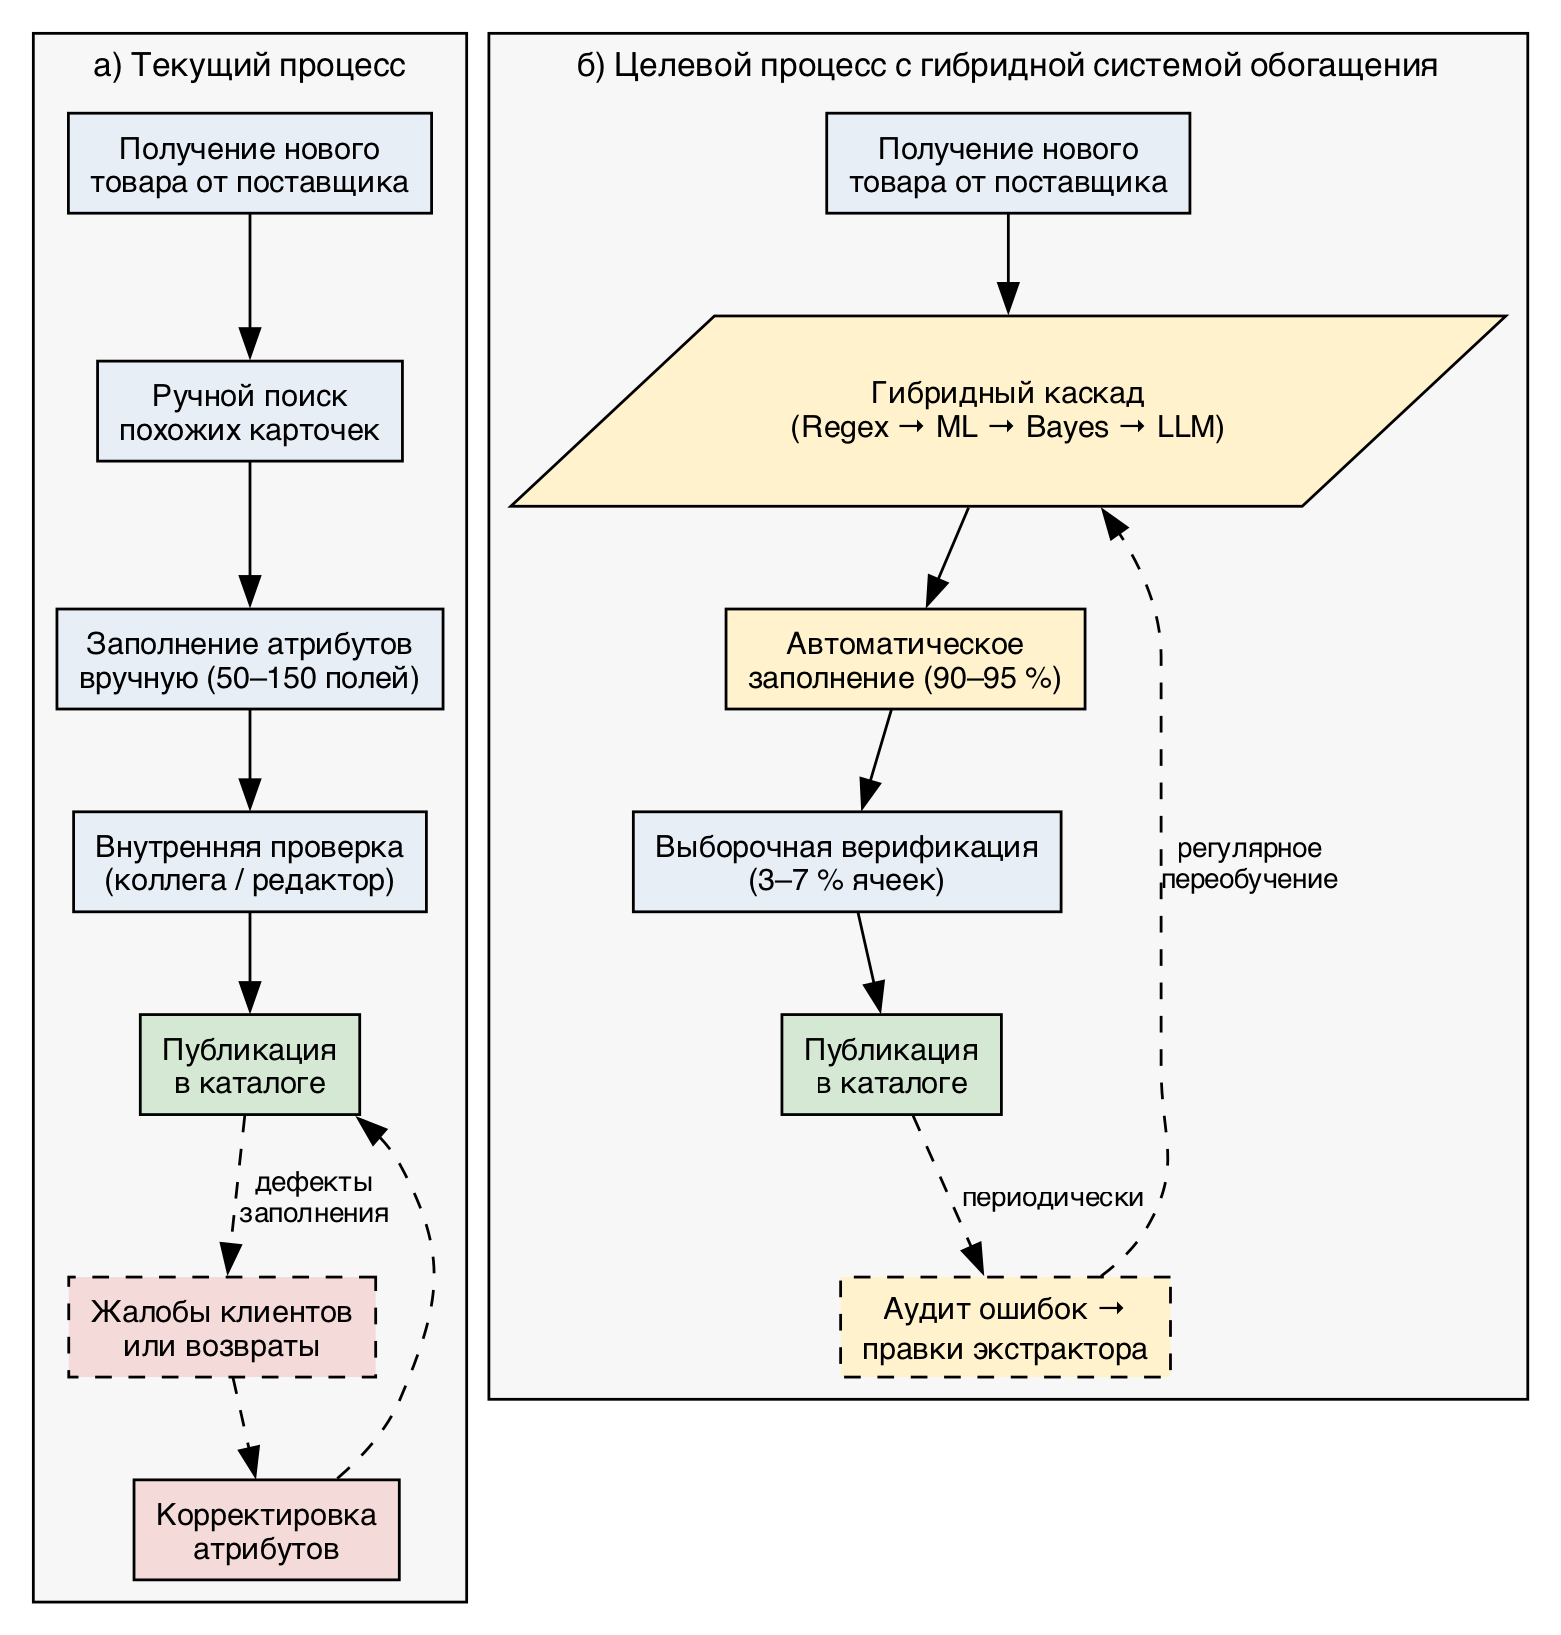
\includegraphics[width=\textwidth]{fig_1_1_cm_process.png}
  \caption{Процесс работы контент-менеджера: (а) текущий, (б) целевой с интеграцией гибридного каскада обогащения}
  \label{fig:fig_1_1_cm_process}
\end{figure}

Примечание. Этапы текущего процесса реконструированы по материалам публичной документации Akeneo \cite{ref_5}, Pimcore \cite{ref_6} и Salsify \cite{ref_7}; целевой процесс — авторская конструкция.

\subsubsection{Эффекты неполной карточки на пользовательский опыт}

Неполная карточка даёт три независимых воздействия: (1) снижается качество фасетного поиска (товар выпадает из подборок при применении фильтров — например, упаковка пасты без формы или типа зерна); (2) растут возвраты и негативная обратная связь, особенно по атрибутам правового или диетического значения (органика, глютен, аллергены); (3) растёт нагрузка на модерацию — «брошенная» карточка удлиняет цикл выхода товара на витрину или порождает повторные правки.

\subsubsection{Существующие системы управления товарной информацией не решают задачу}

Класс систем управления информацией о товарах (PIM, product information management) — Akeneo, Pimcore, Salsify, Riversand, inRiver \cite{ref_5, ref_6, ref_7} — сложился из корпоративной потребности хранить и публиковать товарную информацию в едином каталоге. Их функциональность сосредоточена на управлении уже сформированной информацией, не на её извлечении. Сравнительный анализ платформ управления нормативно-справочной информацией с учётом MDM/PIM-функциональности проведён С. А. Долгоруковой \cite{ref_47}. Появляющиеся модули автоматического обогащения — обёртки над одной публичной большой языковой моделью (LLM, large language model) с прямым вызовом на каждый товар, экономически приемлемые лишь для каталогов небольшого и среднего размера и не дающие гарантий корректности. Альтернатива в виде агрегаторов готовых описаний задачу извлечения атрибутов из произвольного партнёрского текста не решает и ограничена крупными брендами.

\subsubsection{Противоречие и постановка задачи}

Изложенное определяет противоречие в основе актуальности: автоматизация наполнения — инженерная необходимость, но ни одна отдельная технология не покрывает все типы целевых атрибутов с приемлемой точностью и стоимостью. Правила надёжны на числовых атрибутах, но дают низкое покрытие на семантически нагруженных полях. Классические классификаторы требуют значительной разметки и плохо переносятся между языками. LLM универсальны, но дороги \cite{ref_9} и систематически ошибаются на числовых полях, требующих агрегирования из текста (эмпирическая характеристика — 3.3.2.4).

Из противоречия вытекает рабочая архитектурная гипотеза: каскадная композиция слоёв, в которой каждый следующий слой подключается только к остатку, не закрытому предыдущими с заданной уверенностью, способна совместить преимущества отдельных технологий. Проверка этой гипотезы — содержательное ядро работы.

\subsection{Литературный обзор}

В разделе систематизируется научный и индустриальный задел по трём направлениям, которые образуют основу разрабатываемой системы:

извлечение признаков из текстовых описаний товаров;

каскады больших языковых моделей с учётом стоимости вызовов;

существующие промышленные системы управления товарной информацией.

\subsubsection{Извлечение признаков из текстовых описаний товаров}

Задача восполнения пропущенных атрибутов рассматривается как частный случай извлечения признаков из неструктурированного текста (information extraction, IE). Систематизация методов извлечения информации из текста, включая выделение именованных сущностей и фактов, приведена в обзоре Л. М. Ермаковой \cite{ref_51}; гибридная природа практических решений по выделению ключевых слов и признаков из русскоязычных текстов отмечена в работе А. С. Ванюшкина и Л. А. Гращенко \cite{ref_52}. Подходы делятся на три группы — формальные правила, классические статистические модели и нейросетевые модели на трансформерах — и их сочетание образует основу каскадных архитектур.

Правила и регулярные выражения. Формальные шаблоны надёжно извлекают атрибуты с устойчивой лексической разметкой (\% жира, масса нетто, время приготовления, минимальный возраст) при околонулевой стоимости и встроенной интерпретируемости; ограничены низким покрытием на семантически нагруженных полях (тип крупы, форма пасты, маркировка органики).

Статистические модели над поверхностными признаками. Классификаторы поверх TF-IDF (term frequency × inverse document frequency, частотно-инверсный показатель) и градиентный бустинг (XGBoost \cite{ref_14}, LightGBM \cite{ref_15}) работают при достаточной выборке и одноязычном входе. Применение ML к классификации в электронной коммерции рассмотрено Г. И. Афанасьевым и соавторами \cite{ref_16}. Слабая переносимость на многоязычные тексты и отсутствие учёта семантики ограничивают применимость.

Векторные представления на основе трансформеров. Архитектура трансформера \cite{ref_17} и BERT \cite{ref_18} подняли качество IE. Sentence-BERT \cite{ref_19} и многоязычные дистиллированные варианты \cite{ref_20} дают фиксированные представления предложений, поверх которых ставится произвольный классификатор. Категоризация и извлечение признаков из товарных каталогов рассмотрены А. Г. Колониным \cite{ref_21}; систематическое изложение NLP и IE — в учебнике Е. И. Большаковой и соавторов \cite{ref_22}.

Специализированные системы извлечения атрибутов товаров. В индустриальной литературе выделяются три эталонные системы:

\begin{itemize}
    \item TXtract \cite{ref_23} (Karamanolakis et al., ACL 2020, Amazon) — многозадачный нейронный кодировщик с условием на таксономию категорий, обеспечивающий извлечение атрибутов в крупных каталогах при значительном дисбалансе классов;
    \item MAVE \cite{ref_24} (Yang et al., WSDM 2022, Google) — многоисточниковый кодировщик на основе BERT с кросс-вниманием, использующий не только наименование, но и описание, спецификации и другие текстовые поля карточки;
    \item OpenTag \cite{ref_25} (Zheng et al., KDD 2018) — двунаправленная рекуррентная архитектура BiLSTM-CRF с механизмом внимания, формулирующая задачу извлечения атрибутов как задачу разметки последовательности.
\end{itemize}

Эти системы дают 85–92 \% F1 на специализированных корпусах. Сопоставление с каскадными архитектурами, привлекающими LLM в роли запасного слоя, в открытой литературе систематически не представлено: специализированные системы и LLM-каскады трактуются как раздельные направления. Настоящая работа частично закрывает этот пробел.

\subsubsection{Стоимостно-чувствительные каскады больших языковых моделей}

С появлением спектра LLM разной мощности оформилась подобласть cost-aware LLM routing — направление каждого запроса к минимально достаточной модели без потери качества.

FrugalGPT. L. Chen, M. Zaharia и J. Zou \cite{ref_9} предложили каскадную композицию LLM по возрастанию стоимости с прерыванием на первом уверенном ответе: каскад из 3–4 моделей с откалиброванной уверенностью даёт то же качество, что прямой вызов самой дорогой, при стоимости на порядок ниже. Настоящая работа опирается на идеи последовательного прерывания и калибровки.

AutoMix. P. Aggarwal, A. Madaan и соавторы \cite{ref_10} основываются на самопроверке ответа малой моделью с делегированием к большой при сомнении. Разрабатываемая система, наоборот, разносит роли валидатора и предсказателя в раздельные слои.

Hybrid LLM. D. Ding, A. Mallick и соавторы \cite{ref_11} рассматривают маршрутизацию между моделью на пограничном устройстве и облачной — постановка прямо соответствует сценарию «локально развёрнутая gpt-oss-120b + коммерческое API как запасной слой».

RouterBench. Q. J. Hu, J. Bieker и соавторы \cite{ref_12} показали, что обучаемые маршрутизаторы не доминируют над простыми политиками при локализованной структуре ошибок. На задаче обогащения каталогов в настоящей работе впервые по протоколу, зафиксированному до получения результатов установлено, что статическое per-(категория, атрибут) правило не уступает обучаемому маршрутизатору по сквозной точности при равном бюджете запасного слоя.

\subsubsection{Существующие промышленные PIM-системы и анализ аналогов}

Для позиционирования разработки относительно индустриальных аналогов отобраны три коммерческие PIM-системы: Akeneo, Pimcore и Salsify. По ним построена сравнительная таблица по семи функциональным критериям, существенным для задачи автоматического обогащения каталога (таблица 1.1). Источниками послужила документация вендоров \cite{ref_5, ref_6, ref_7}.

\begin{xltabular}{\textwidth}{|X|X|X|X|X|X|}
\caption{Сравнение существующих PIM-систем и разрабатываемой системы} \\ \hline
    № & Критерий & Akeneo & Pimcore & Salsify & Разрабатываемая система \\ \hline
\endfirsthead
\multicolumn{6}{l}{\textit{Продолжение таблицы}} \\ \hline
    № & Критерий & Akeneo & Pimcore & Salsify & Разрабатываемая система \\ \hline
\endhead
    1 & Централизованное хранение каталога & да & да & да & не входит в задачу \\ \hline
    2 & Распределение по каналам сбыта & да & да & да & не входит в задачу \\ \hline
    3 & Автоматическое обогащение атрибутов & нет (только ручная редактура) & частично (правила обогащения) & нет (есть AI Suite как обёртка над сторонней LLM) & да (каскадная архитектура) \\ \hline
    4 & Извлечение признаков из неструктурированного текста & нет & нет & нет & да (слои ML и LLM) \\ \hline
    5 & Поддержка многоязычного входа & через ручные переводы & через ручные переводы & через ручные переводы & встроенная (многоязычные эмбеддинги, 50+ языков) \\ \hline
    6 & Открытый исходный код & community-редакция & да & нет & да (включая возможность локального развёртывания LLM) \\ \hline
    7 & Стоимостно-чувствительная обработка & нет & нет & нет & да (каскадная композиция с доминированием по Парето по стоимости и качеству) \\ \hline
\end{xltabular}

Из таблицы 1.1 следует, что коммерческие PIM-системы хорошо покрывают хранение, версионирование и распределение уже сформированной информации. Однако они систематически не решают задачи извлечения атрибутов из произвольного партнёрского текста. Появляющаяся функция автоматического обогащения реализуется как обёртка над сторонней языковой моделью. Таким образом, ни одно из проанализированных решений не закрывает одновременно весь набор критериев интернет-магазина: автоматическое обогащение, многоязычную обработку, контролируемую стоимость и возможность локального развёртывания. Это обосновывает целесообразность разработки самостоятельной системы.

\subsubsection{Слабый надзор, калибровка и сопутствующая методология}

Принципиальная сложность задачи — отсутствие достаточной ручной разметки; постановка известна как weak supervision, инструментарий систематизирован A. Ratner и соавторами «Snorkel» \cite{ref_26}. Подходы к снижению стоимости разметки через активное обучение и слабый надзор систематизированы в обзоре B. Settles \cite{ref_46}. Пригодным источником слабого эталона выступает Open Food Facts \cite{ref_13} — открытая база >4,5 млн пищевых продуктов с пользовательскими тегами. Эмпирический анализ устойчивости алгоритмов классификации к зашумлению обучающей разметки выполнен В. А. Дюком \cite{ref_48} и показал, что классические методы (KNN, SVM) сохраняют приемлемую точность при умеренной доле ошибок разметки, что обосновывает применимость серебряной разметки.

Для корректной работы каскада выходы классификаторов должны быть откалиброваны: масштабирование Платта \cite{ref_27}, изотоническая регрессия \cite{ref_28}; современный анализ ECE для глубоких моделей — C. Guo и соавторы \cite{ref_29}. Систематизация критериев качества классификаторов (включая ROC-анализ и выбор порога вероятности) дана в работах Ю. С. Шуниной и соавторов \cite{ref_49} и А. А. Ковалева и соавторов \cite{ref_50}. Оценка точности при ограниченной выборке — кросс-валидация и бутстрэп \cite{ref_30}; интервальная оценка пропорций — формула Вильсона \cite{ref_31}.

Аппарат байесовских сетей опирается на J. Pearl \cite{ref_32}, D. Heckerman et al. \cite{ref_33}, А. Л. Тулупьева и соавторов \cite{ref_34}, библиотеку pgmpy \cite{ref_35}; поиск структуры — Hill Climb + BIC \cite{ref_36}. Прикладные вопросы устойчивости ML-моделей к дрейфу в розничных каталогах рассмотрены А. А. Артемовым \cite{ref_37}; ограниченная масштабируемость стандартных подходов к управлению ассортиментом на маркетплейсах — С. А. Сергеев \cite{ref_38}; активное обучение и краудсорсинг — Р. А. Гилязев и Д. Ю. Турдаков \cite{ref_39}; ранние работы по семантическим пространствам — В. Ф. Хорошевский \cite{ref_40}.

\subsection{Техническое задание на разрабатываемую систему}

В разделе формулируется техническое задание (ТЗ) на разрабатываемую систему. Оно подразделяется на три группы требований: функциональные (что система должна делать), нефункциональные (с какими характеристиками) и архитектурные (каким способом она организована).

\subsubsection{Функциональные требования}

\textbf{Ф-1. Принимаемый формат входных данных.} Система принимает на входе товар, описанный полями партнёра-поставщика:

наименование (product\_name);

бренд (brands);

список ингредиентов в произвольной форме (ingredients\_text);

масса, объём или упаковка (quantity);

идентификатор категории (category), опционально.

Все поля, кроме наименования, считаются необязательными.

\textbf{Ф-2. Возврат заполненных значений целевых атрибутов.} Система возвращает для каждого целевого атрибута предсказанное значение, оценку уверенности и идентификатор слоя каскада, на котором принято финальное решение. Тем самым обеспечивается отслеживаемость источника каждого предсказания и возможность ручной верификации контент-менеджером.

\textbf{Ф-3. Покрытие предметных категорий.} В пределах работы система поддерживает заполнение целевых атрибутов для трёх категорий пищевой продукции: паста, шоколад и шоколадные изделия, сыры. Выбор именно этих трёх категорий обоснован тремя причинами. Во-первых, в Open Food Facts по ним имеется достаточный объём обучающих данных. Во-вторых, доступен аудит-эталон с согласием трёх больших языковых моделей и слепой разметкой Opus. В-третьих, сами категории репрезентативны с точки зрения распределения типов целевых атрибутов: числовых, бинарных и мультиклассовых семантических.

\textbf{Ф-4. Автоматическое определение категории.} Если категория явно не указана, система определяет её автоматически по поступившему текстовому описанию товара. Эта функция реализуется отдельным предкаскадным слоем (Слой 0).

\textbf{Ф-5. Запасной слой на основе большой языковой модели.} Если получить однозначный ответ на конкретный атрибут средствами слоёв 1–3 каскада не удаётся, система обращается к большой языковой модели как к запасному слою. Запасной слой подключается селективно: только для тех атрибутов конкретного товара, по которым предыдущие слои не выдали уверенного ответа.

\textbf{Ф-6. Диагностический вывод.} Система возвращает диагностическую информацию: результат работы валидатора (понижение или подтверждение предсказания), агрегированные оценки уверенности по слоям и маршрут запроса по каскаду. Эта информация необходима для отладки, аудита и накопления данных о поведении системы в эксплуатации.

\subsubsection{Нефункциональные требования}

\textbf{НФ-1. Точность.} Целевая сквозная точность каскада на эталонной тестовой выборке без пересечения товарных кодов между обучающей и тестовой частями (code-disjoint, новые SKU) — не менее 85 \%. В конфигурации с коммерческой большой языковой моделью в запасном слое — не менее 90 \%.

\textbf{НФ-2. Стоимость.} Стоимость обработки одного товара каскадом должна быть существенно ниже стоимости прямого вызова большой языковой модели на тот же товар. Целевой коэффициент снижения — не менее 2,5×. Ограничение сверху не задаётся; фактически достижимое значение фиксируется по результатам эмпирической оценки в 3.3.2.

\textbf{НФ-3. Производительность.} Время отклика на один товар при работе без обращения к запасному слою — не более 500 мс на потребительском ноутбуке без специализированного ускорителя. При необходимости обращения к запасному слою — не более 5 секунд. Это значение определяется временем ответа внешнего API большой языковой модели.

\textbf{НФ-4. Многоязычность.} Система поддерживает обработку описаний товаров на пяти рабочих языках европейского рынка пищевой продукции: французском, английском, немецком, итальянском и испанском. Это соответствует наиболее представленным языкам в Open Food Facts и моделирует реалистичный многоязычный партнёрский поток.

\textbf{НФ-5. Возможность локального развёртывания.} Система поддерживает сценарий полностью локального развёртывания, при котором обращения к внешним коммерческим API исключаются. Этот сценарий реализуется через подключение в запасной слой открытой языковой модели gpt-oss-120b. Тем самым к каскаду предъявляется требование вендорной независимости.

\subsubsection{Архитектурные требования}

\textbf{А-1. Каскадная архитектура с раздельными слоями.} Система реализует последовательность слоёв обработки по принципу «передачи остатка». Каждый последующий слой обрабатывает только те атрибуты, по которым предыдущие слои не выдали ответа с уверенностью выше калиброванного порога. Архитектурно слои разделены и могут обновляться независимо.

\textbf{А-2. Независимое обновление слоёв.} Изменение или переобучение любого отдельного слоя не должно требовать перезапуска или повторного развёртывания других слоёв и API-шлюза системы. К таким изменениям относятся обновление правил, дообучение классификаторов слоя 2, замена языковой модели в запасном слое.

\textbf{А-3. Демонстрационный программный комплекс с веб-интерфейсом.}  Система сопровождается демонстрационным комплексом, который состоит из трёх компонентов:

API-шлюз на языке Go;

ML-сервис на языке Python (FastAPI);

одностраничный веб-интерфейс.

Демонстрация обеспечивает верификацию работоспособности и наглядно представляет результаты работы каскада для контент-менеджера.

\subsubsection{Соотношение технического задания и решаемых задач работы}

Сформулированные требования полностью покрываются задачами, поставленными во введении (таблица 1.2).

\begin{xltabular}{\textwidth}{|X|X|X|}
\caption{Соответствие требований технического задания и задач работы} \\ \hline
    № задачи & Краткая формулировка задачи & Покрываемые требования ТЗ \\ \hline
\endfirsthead
\multicolumn{3}{l}{\textit{Продолжение таблицы}} \\ \hline
    № задачи & Краткая формулировка задачи & Покрываемые требования ТЗ \\ \hline
\endhead
    1 & Разработать архитектуру гибридного каскадного конвейера & Ф-1, Ф-2, Ф-4, Ф-5, А-1 \\ \hline
    2 & Реализовать каждый слой каскада как самостоятельный программный компонент & Ф-6, А-2 \\ \hline
    3 & Построить эталонную разметку и проверочную выборку без пересечения товарных кодов (code-disjoint) & Ф-3 (в части обеспечения данных для оценки на трёх категориях) \\ \hline
    4 & Провести экспериментальную оценку точности, покрытия и стоимости & НФ-1, НФ-2, НФ-3, НФ-4, НФ-5 \\ \hline
    5 & Разработать демонстрационный программный комплекс & А-3 \\ \hline
\end{xltabular}

Установленное соответствие подтверждает, что выполнение пяти задач работы влечёт за собой выполнение технического задания в полном объёме.

\subsection{Выводы по главе 1}

В главе проведён анализ предметной области, систематизировано состояние литературы и обосновано техническое задание. По результатам анализа можно сформулировать следующие выводы.

\begin{enumerate}[arabic]
    \item Проблема автоматического обогащения остаётся открытой. Промышленные PIM-системы, такие как Akeneo \cite{ref_5}, Pimcore \cite{ref_6}, Salsify \cite{ref_7}, ориентированы на хранение и распределение уже сформированной информации. Появляющиеся модули автоматического обогащения реализуются как обёртки над одной коммерческой большой языковой моделью и не отвечают требованиям обработки больших каталогов с учётом стоимости.
    \item Научные подходы делятся на две группы, и ни одна из них не покрывает задачу полностью. Специализированные системы извлечения атрибутов, такие как TXtract \cite{ref_23}, MAVE \cite{ref_24}, OpenTag \cite{ref_25}, решают задачу с высоким качеством. Однако они требуют значительной размеченной выборки и не учитывают экономики обращения к моделям. Каскады больших языковых моделей с учётом стоимости — FrugalGPT, AutoMix, Hybrid LLM — дают инструменты управления стоимостью, систематически сопоставленные в бенчмарке RouterBench. Однако эти каскады рассматривают композицию из однородных моделей и не интегрируют классическое машинное обучение.
    \item Разрабатываемая система объединяет оба подхода в гибридный каскад. Каскад сочетает специализированные слои извлечения признаков — правила, машинное обучение на многоязычных эмбеддингах, байесовский валидатор — и запасной слой LLM с учётом стоимости. Совокупность шести функциональных, пяти нефункциональных и трёх архитектурных требований ТЗ формирует обязательство, выполнение которого верифицируется в экспериментальной части работы.
\end{enumerate}
        % Глава 1
    
\section{ТЕОРЕТИЧЕСКОЕ ОБОСНОВАНИЕ РЕШЕНИЯ}

В главе формально описывается разрабатываемая система и обосновываются принятые архитектурные решения. Сначала приводится формальная постановка задачи и логика работы программного обеспечения (2.1). Затем рассматриваются архитектура и стек технологий, обоснование выбора каждой компоненты (2.2). В конце разбирается прохождение типового запроса через систему (2.3).

\subsection{Логика работы разрабатываемого программного обеспечения}

\subsubsection{Формальная постановка задачи обогащения}

Пусть товарная позиция, поступающая в систему от партнёра, представлена кортежем партнёр-доступных полей

\begin{equation}
\label{eq:2.1}
x = (x^{\text{name}}, x^{\text{brand}}, x^{\text{ingr}}, x^{\text{qty}}),
\end{equation}

где компоненты — название, бренд, состав и количество соответственно; пустым может быть любое поле, кроме названия. Каждому товару ставится в соответствие категория $c \in \mathcal{C} = \{c_1, \dots, c_M\} \cup \{\text{OOD}\}$ ($M = 3$: pasta, chocolate, cheeses; OOD — выход за пределы поддерживаемых доменов), определяемая отдельной моделью

\begin{equation}
\label{eq:2.2}
c = f_0(x),
\end{equation}

(Слой 0, см. 2.2.1). Для каждой категории задана схема $\mathcal{A}_c = \{a_1, \dots, a_{K_c}\}$ с областями $\mathcal{Y}_k$; система строит

\begin{equation}
\label{eq:2.3}
\hat{y} = (\hat{y}_1, \dots, \hat{y}_{K_c}) \in (\mathcal{Y}_1 \cup \{\text{null}\}) \times \dots \times (\mathcal{Y}_{K_c} \cup \{\text{null}\}),
\end{equation}

где $\hat{y}_k = \text{null}$ — явный отказ от ответа. Честное молчание лучше неверного заполнения: повторное обращение к оператору дешевле ошибки на витрине.

\subsubsection{Каскадная схема принятия решения}

Логика обогащения реализована как каскад из четырёх содержательных слоёв; ему предшествует определение категории. Для каждого атрибута $k$ итоговое предсказание формируется по правилу

\begin{gather}
\label{eq:2.4}
\hat{y}_k =
\begin{cases}
f_k^{\text{regex}}(x), & f_k^{\text{regex}}(x) \neq \varnothing; \\[4pt]
f_k^{\text{ML}}(x), & f_k^{\text{regex}}(x) = \varnothing,\ P_{\text{ML}}(\hat{y}_k \mid x) \geq \tau_k,\ P_B(\hat{y}_k \mid \mathbf{e}) \geq \theta_k; \\[4pt]
f_k^{\text{LLM}}(x), & \text{otherwise}.
\end{cases}
\end{gather}

Здесь $f_k^{\text{regex}}$ — детерминированный экстрактор регулярных выражений (Слой 1); $f_k^{\text{ML}}$ — классификатор машинного обучения (Слой 2) над многоязычным векторным представлением партнёр-доступных полей с калиброванной апостериорной вероятностью $P_{\text{ML}}$ и поатрибутным порогом $\tau_k$; $P_B(\hat{y}_k \mid \mathbf{e})$ — оценка байесовской сети при свидетельствах $\mathbf{e} = (x^{\text{brand}}, \hat{y}_{j \neq k})$ с порогом $\theta_k$, заданным как пятый перцентиль распределения $P_B$ по верно размеченным обучающим примерам; $f_k^{\text{LLM}}$ — запасной слой на большой языковой модели (LLM, large language model), возвращающий значение из $\mathcal{Y}_k$ или $\text{null}$. Предсказание Слоя 2 принимается тогда и только тогда, когда одновременно выполнены

\begin{equation}
\label{eq:2.5}
\bigl[P_{\text{ML}}(\hat{y}_k \mid x) \geq \tau_k\bigr] \ \wedge\ \bigl[P_B(\hat{y}_k \mid \mathbf{e}) \geq \theta_k\bigr].
\end{equation}

Это конъюнктивное условие формализует требование темы об ансамблевой оценке уверенности: не параллельное голосование, а последовательная фильтрация с правом каждого слоя отказаться. По итогам 3.3.4 валидатор включён точечно — только на парах «категория — атрибут» с неотрицательным приростом. Схема даёт ступенчатое распределение нагрузки (дешёвый Слой 1 — массовые случаи, дорогой Слой 4 — трудный остаток), отбраковку статистически маловероятных пар «бренд × значение» и архитектурную объяснимость: для каждой ячейки известно, какой слой принял решение.

\subsubsection{Поведение системы при выходе категории за пределы поддерживаемых}

Слой 0 определяет $c = f_0(x)$ до запуска каскада. Если уверенность ниже порога OOD-детектора, товару присваивается метка OOD и система возвращает «категория не поддерживается»: $f_0(x) \in \mathcal{C} \setminus \{\text{OOD}\} \Rightarrow$ запуск per-category каскада со схемой $\mathcal{A}_{f_0(x)}$; $f_0(x) = \text{OOD} \Rightarrow \hat{y} = \varnothing$. Явный отказ выбран по соображениям эксплуатационной безопасности: если товар ошибочно отнести к чужой категории, всем атрибутам достанется неверная схема.

\subsubsection{Метрики качества и стоимости}

Каскад поддерживает явный отказ от ответа; используются две согласованные метрики качества и одна сводная по стоимости.

\begin{equation}
\label{eq:2.6}
\text{acc}_k^{\text{cov}} = \frac{\bigl|\{i : \hat{y}_k^{(i)} = y_k^{(i)} \ \wedge\ \hat{y}_k^{(i)} \neq \text{null}\}\bigr|}{\bigl|\{i : \hat{y}_k^{(i)} \neq \text{null}\}\bigr|}.
\end{equation}

Точность на покрытой части $\text{acc}_k^{\text{cov}}$ — доля верных предсказаний среди ячеек с непустым ответом.

\begin{equation}
\label{eq:2.7}
\text{cov}_k = \frac{\bigl|\{i : \hat{y}_k^{(i)} \neq \text{null}\}\bigr|}{N},
\end{equation}

Покрытие $\text{cov}_k$ — доля ячеек, на которых система решилась дать ответ (где $N$ — мощность проверочной выборки).

\begin{equation}
\label{eq:2.8}
\text{acc}_k^{\text{e2e}} = \text{acc}_k^{\text{cov}} \cdot \text{cov}_k.
\end{equation}

Сквозная точность $\text{acc}_k^{\text{e2e}}$ — основная метрика и заголовочное число (3.3.2); ячейки с $\hat{y}_k^{(i)} = \text{null}$ засчитываются как неверные, что не даёт системе завысить качество за счёт молчания.

\begin{equation}
\label{eq:2.9}
\text{cost}_{\text{LLM}} = \frac{1000}{N \cdot K_c} \sum_{i=1}^{N} \sum_{k=1}^{K_c} \mathbb{1}\bigl[\hat{y}_k^{(i)} \text{ получен через } f_k^{\text{LLM}}\bigr].
\end{equation}

Стоимость $\text{cost}_{\text{LLM}}$ — ожидаемая доля вызовов запасного слоя на 1000 ячеек; метрика инвариантна к выбору модели Слоя 4 и характеризует структуру каскада. Совместный анализ $(\text{acc}^{\text{e2e}}, \text{cost}_{\text{LLM}})$ даёт матрицу «точность — стоимость», на которой строится заголовочный результат (3.3.2).

\subsection{Архитектура и стек технологий}

В разделе описывается архитектурное решение, реализующее формальную постановку 2.1, и обосновывается выбор каждой компоненты стека.

\subsubsection{Архитектура системы}

Функциональная модель системы в виде диаграммы потоков данных приведена на рисунке 2.1. Внешние акторы (партнёр-продавец и витрина каталога интернет-магазина) обмениваются данными со шлюзом API и ML-сервисом, который содержит каскад из пяти слоёв и обращается к хранилищам моделей XGBoost, байесовских сетей и внешнему API большой языковой модели.

\begin{figure}
  
\includegraphics[width=\textwidth]{fig_2_1_functional_model.png}
  \caption{Функциональная модель системы обогащения товарных данных}
  \label{fig:fig_2_1_functional_model}
\end{figure}

Система реализована как пятислойный конвейер (Слой 0 + четыре содержательных слоя). Состав и роль каждого слоя:

\begin{itemize}
    \item \textbf{Слой 0 — категорайзер.} LightGBM поверх TF-IDF-представления (term frequency × inverse document frequency, частотно-инверсный показатель) названия и бренда с порогом OOD; определяет $c \in \mathcal{C}$ либо относит к OOD.
    \item \textbf{Слой 1 — экстрактор регулярных выражений.} Извлекает значения, явно присутствующие в тексте (форма пасты, \% какао, цельнозерновой, шаблоны количества). Применяется только к шаблонам с высокой точностью совпадения.
    \item \textbf{Слой 2 — классификатор машинного обучения.} Основной слой: партнёр-доступные поля конкатенируются и кодируются SBERT в 768-мерный вектор (модель paraphrase-multilingual-mpnet-base-v2, архитектура MPNet); поатрибутный XGBoost с порогом $\tau_k$ на отложенной выборке. Изотоническая пост-калибровка исследована в двух режимах (3.3.3.3): серебряная деградирует на эталоне из-за дрейфа; перекрёстная на эталонной выборке даёт улучшение ECE с 0,070 до 0,043 (в производственную конфигурацию не включена).
    \item \textbf{Слой 3 — байесовский валидатор.} Сеть (структура — Hill Climb + BIC) вычисляет $P_B(\hat{y}_k \mid \mathbf{e})$; ниже порога $\theta_k$ — флаг и передача дальше. Роль пересмотрена (3.1): не классификатор, а валидатор плотностей.
    \item \textbf{Слой 4 — запасной слой на большой языковой модели.} Взаимозаменяемые модели семейств GPT \cite{ref_41} и Claude \cite{ref_42}: Sonnet 4.5, GPT-4o, Gemini 2.5 Flash, открытая gpt-oss-120b, малая llama-3.2-3b (сопоставление — 3.3.2). Структурированный запрос со схемой и партнёр-доступными полями; возвращает значение или честный отказ.
\end{itemize}

Слои упорядочены по росту удельной стоимости решения: регулярные выражения почти бесплатны, ML работает на уже вычисленном векторном представлении, байесовский вывод требует одного прохода по сети, запасной слой — самый дорогой.

Структура обученной байесовской сети для категории \texttt{chocolate} приведена на рисунке~\ref{fig:bayes_dag_ch2}. Узлы графа — целевые атрибуты и бренд; направленные рёбра показывают условные зависимости, найденные алгоритмом Hill Climb на серебряной выборке. Бренд — корневой узел; через производный признак \texttt{brand\_has\_organic\_marker} он влияет на \texttt{chocolate\_type} и \texttt{is\_organic}. Тип шоколада задаёт процент какао и подтип \texttt{chocolate\_extra}, от которого расходятся рёбра к \texttt{contains\_nuts}, \texttt{nutri\_score\_grade}, \texttt{protein\_class} и повторно к \texttt{is\_organic} — это согласуется с интуицией о связи органичности, бренда и подтипа. Эмпирическая роль сети как точечного валидатора и количественные характеристики приведены в 3.3.4.

\begin{figure}
  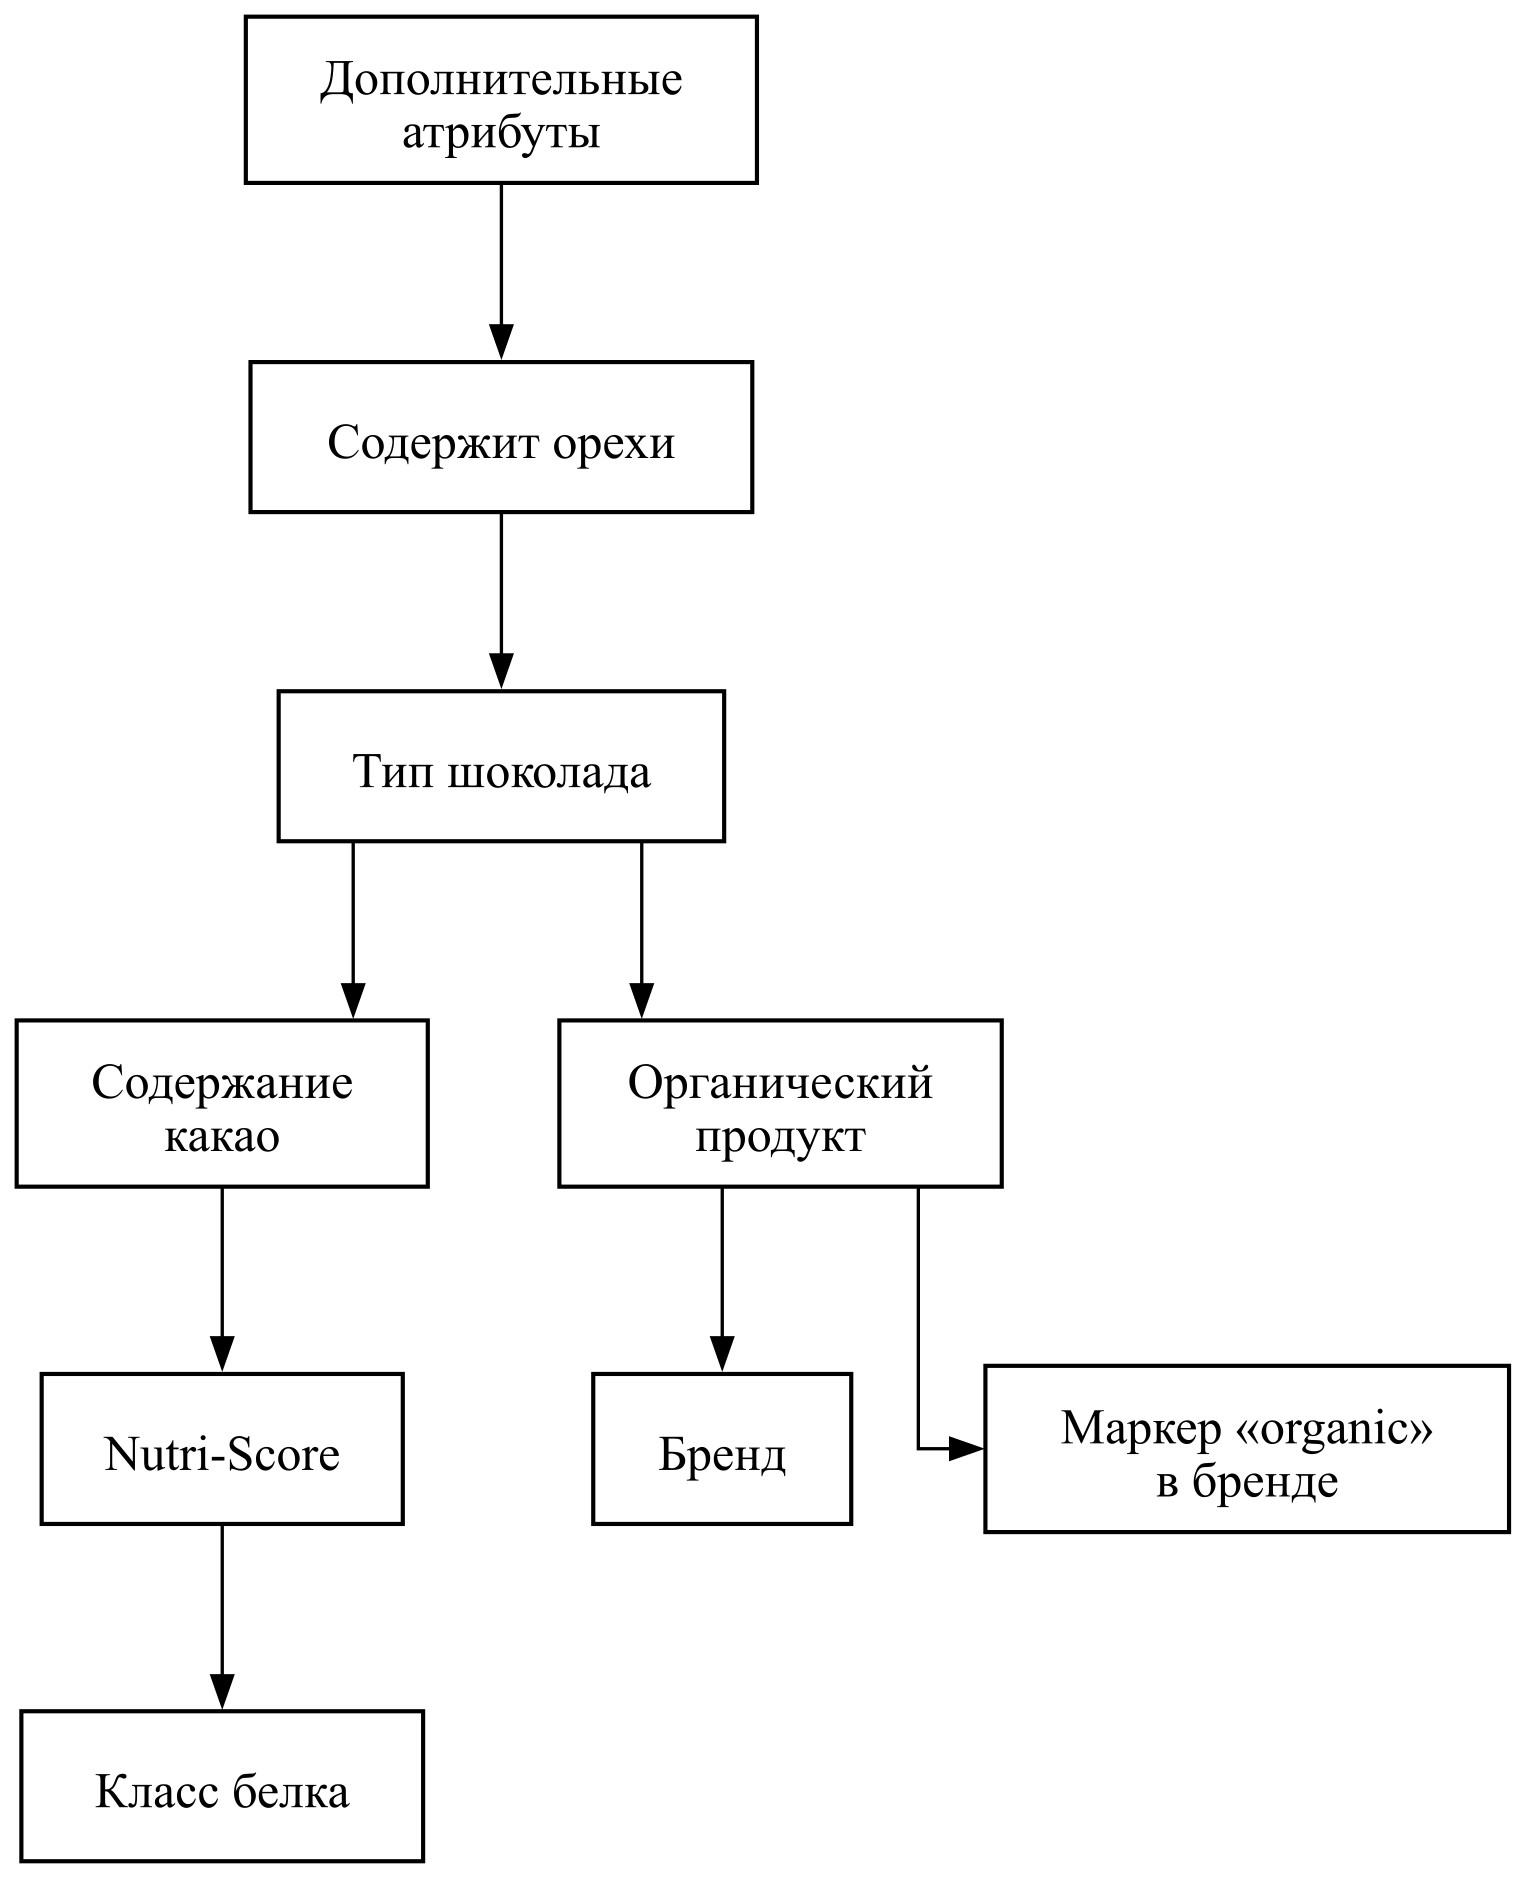
\includegraphics[width=0.8\textwidth]{fig_3_5_bayes_dag.png}
  \caption{Структура байесовской сети категории \texttt{chocolate} (направленный ациклический граф; алгоритм Hill Climb с критерием BIC, библиотека pgmpy 1.1.2)}
  \label{fig:bayes_dag_ch2}
\end{figure}

\subsubsection{Обоснование выбора компонентов стека}

\textbf{Каскад вместо сквозного решения.} Сквозной all-LLM даёт 83--94~\% точности (3.3.2), но стоимость линейно растёт с числом ячеек; каскад при равной или большей точности экономит порядка двух порядков за счёт ступенчатого распределения нагрузки. Сквозной all-ML не подходит — у части атрибутов значения вычисляются из данных за пределами товарного описания, к тому же есть сценарий холодного старта новых категорий.

\textbf{SBERT \texttt{paraphrase-multilingual-mpnet-base-v2}} \cite{ref_20} выбран за бесплатную многоязычность (50+ языков в едином пространстве без дообучения), умеренную 768-мерную размерность и готовность к работе без доменной адаптации. Архитектура MPNet объединяет преимущества маскированного и перестановочного языкового моделирования и устойчиво обгоняет дистиллированные MiniLM-варианты на задачах семантической близости.

\textbf{XGBoost} \cite{ref_14} с регуляризацией (subsample=0.8, colsample=0.8, ранняя остановка, gamma=0.1) выбран как Слой 2 за устойчивость на плотных векторных признаках при ограниченной разметке (n$\approx$1250 на категорию), калибруемость вероятностей (изотоническая регрессия \cite{ref_28}) и миллисекундный вывод на CPU. Поэтапная оптимизация по остаткам и явные L1/L2/$\gamma$-штрафы дают более тонкие нелинейные границы и более прямой контроль переобучения, чем у Random Forest~\cite{ref_53,ref_54}; на независимых табличных стендах \cite{ref_55,ref_56} градиентный бустинг устойчиво обходит Random Forest и нейросетевые архитектуры в характерной для Слоя 2 размерности. Эмпирическое сравнение (\S\,\ref{sec:method-comparison}) подтверждает выбор: при сопоставимой точности XGBoost даёт наименьшую ECE (0,026 против 0,031 у MLP и 0,035 у LogReg).

\textbf{Байесовская сеть на pgmpy \cite{ref_35} 1.1.2.} По сравнению с MRF и автоэнкодерами дискретная байесовская сеть допускает построение структуры графа (Hill Climb + BIC \cite{ref_36}) с интерпретируемым ориентированным графом, дешёвый вывод через Variable Elimination и явное выражение условных зависимостей; pgmpy поддерживает и построение структуры, и оценку параметров через \texttt{BayesianEstimator}.

\textbf{Шлюз API на Go при ML-сервисе на Python.} Демо-система — два сервиса: шлюз на Go (\texttt{:8080}) и ML-сервис на Python/FastAPI (\texttt{:8001}). Go подходит для сетевого ввода-вывода (малое потребление памяти, быстрый запуск, конкурентный I/O); Python-экосистема (PyTorch, sentence-transformers, XGBoost, pgmpy) безальтернативна для ML-инференса. Разделение соответствует типовой производственной архитектуре и позволяет масштабировать компоненты независимо.

\textbf{Открытая LLM как запасной слой.} Конфигурация многомодельна через OpenRouter (Claude Sonnet 4.5, GPT-4o, Gemini 2.5 Flash, открытая gpt-oss-120b, малая llama-3.2-3b). Открытую gpt-oss-120b можно запустить в инфраструктуре заказчика без передачи данных вовне; коммерческие LLM взаимозаменяемы, что снижает зависимость от провайдера; каскад компенсирует слабость малой модели — при самостоятельном применении gpt-oss-120b проигрывает Sonnet 14--15~п.~п., но в составе каскада превосходит её безусловное использование на 21,3~п.~п. (3.3.2).

\subsubsection{Стек технологий — сводная таблица}

Сводное представление принятых решений приведено в таблице 2.1.

\begin{xltabular}{\textwidth}{|>{\raggedright\arraybackslash}p{3.0cm}|>{\raggedright\arraybackslash}p{5.5cm}|>{\raggedright\arraybackslash}X|}
\caption{Сводная таблица стека технологий с обоснованием выбора} \\ \hline
    Компонент & Технология & Ключевое обоснование \\ \hline
\endfirsthead
\multicolumn{3}{l}{Продолжение таблицы} \\ \hline
    Компонент & Технология & Ключевое обоснование \\ \hline
\endhead
    Шлюз API & Go, стандартная библиотека net/http & Малое потребление ресурсов, быстрый запуск, отсутствие внешних зависимостей \\ \hline
    ML-сервис & Python 3.14, FastAPI, Uvicorn & Доступ к ML-экосистеме, автоматическая валидация через Pydantic, поддержка OpenAPI \\ \hline
    Векторное представление & SBERT \texttt{paraphrase-\allowbreak multilingual-\allowbreak mpnet-\allowbreak base-v2} & Многоязычность (50+ языков), 768-мерный вектор (архитектура MPNet), отсутствие необходимости в дообучении \\ \hline
    Классификатор Слой 2 & XGBoost с регуляризацией; перекрёстная изотоническая калибровка на эталонной выборке снижает среднюю ECE с 0,070 до 0,043 (3.3.3.3), внедрение в производственную конфигурацию вынесено в раздел «Перспективы развития темы» заключения & Устойчивость на плотных признаках, калибруемые вероятности, дешёвый вывод \\ \hline
    Байесовская сеть & pgmpy 1.1.2, \texttt{Discrete}\allowbreak\texttt{BayesianNetwork} & Структурное обучение Hill Climb + BIC, дешёвый вывод (Variable Elimination), интерпретируемый граф \\ \hline
    Категорайзер Слой 0 & LightGBM (поверх TF-IDF-представления) + порог OOD & Многоклассовая классификация с вероятностями + явный отказ при низкой уверенности \\ \hline
    Запасной слой & OpenRouter API: Sonnet 4.5, GPT-4o, Gemini 2.5 Flash, gpt-oss-120b, llama-3.2-3b & Единый интерфейс, возможность локального развёртывания, независимость от поставщика \\ \hline
    Фронтенд & HTML/CSS/JavaScript без сборочной системы & Минимальные требования к окружению, прозрачность демонстрации \\ \hline
\end{xltabular}

\subsection{Сценарий работы программного обеспечения}

\subsubsection{Сквозной пример прохождения запроса}

Рассмотрим прохождение на примере «Spaghetti \#5 Barilla» (повторяется в 3.1.2). Партнёр шлёт \texttt{POST /api/enrich} с полями category=null, product\_name=«Spaghetti \#5 Barilla», brands=«Barilla», ingredients\_text=«Durum wheat semolina, water», quantity=«500g». Поле category пустое — категоризация на системе.

\textbf{Шаг 1. Определение категории (Слой 0).} Возвращает $c = \text{pasta}$ с уверенностью $0{,}97$; OOD не сработал, выбрана схема $\mathcal{A}_{\text{pasta}}$ (8 атрибутов).

\textbf{Шаг 2. Поочерёдная обработка атрибутов.} Каскад обходит атрибуты по схеме. Для pasta\_shape срабатывает шаблон Слоя 1 на «spaghetti» с уверенностью $1{,}0$ — следующие слои не вызываются. Для grain\_type Слой 1 не даёт совпадения; Слой 2 выдаёт \texttt{"wheat"} с $P_{\text{ML}} = 0{,}99 \geq \tau = 0{,}5$, валидатор подтверждает ($P_B = 0{,}85 \geq \theta = 0{,}04$) — отметка ml. Для nutri\_score\_grade — класс \texttt{"A"}, $P_{\text{ML}} = 0{,}83$, валидатор подтверждает. Для is\_filled $P_{\text{ML}} = 0{,}45 < \tau$ — ячейка идёт в Слой 4.

\textbf{Шаг 3. Формирование ответа.} ML-сервис собирает поатрибутный ответ с агрегированными счётчиками и возвращает JSON шлюзу (формат — 3.1.2). В этом сценарии 7 из 8 атрибутов закрыты дешёвыми слоями (1 regex + 6 ML), 1 — Слоем 4. Именно такое распределение и даёт каскаду выигрыш в матрице «точность — стоимость» (3.3.2).

\subsection{Выводы по главе 2}

\begin{enumerate}[label=\arabic*)]
    \item Задача обогащения формализована как поатрибутное предсказание $\hat{y}_k$ с явным отказом ($\hat{y}_k = \text{null}$); каскадная логика — последовательная фильтрация по уверенности с конъюнктивным условием $P_{\text{ML}} \geq \tau_k \wedge P_B \geq \theta_k$ для принятия предсказания Слоя 2 как ансамблевая оценка уверенности.
    \item Архитектурный выбор каждой компоненты (каскад вместо сквозного решения; SBERT, XGBoost, pgmpy; Go-шлюз + Python-ML; открытая gpt-oss-120b) обоснован эксплуатационно, методологически и стратегически. Это превращает слабую открытую модель в работоспособную часть производственного стека.
    \item Сквозной сценарий подтверждает: большинство атрибутов закрывается дешёвыми слоями, обращение к LLM точечно — отсюда и доминирование каскада по Парето над одиночным вызовом большой языковой модели (подтверждается в 3.3).
\end{enumerate}
          % Глава 2
    
\section{ОПИСАНИЕ ПРОГРАММНО-ТЕХНОЛОГИЧЕСКОЙ РЕАЛИЗАЦИИ}

Глава описывает программную реализацию системы: 3.1 — каскад и демонстрационный комплекс; 3.2 — данные и предобработку; 3.3 — численные результаты и сценарии тестирования.

\subsection{Описание программного обеспечения}

\subsubsection{Архитектура каскада}

Гибридный каскад — последовательность из пяти слоёв; каждый обрабатывает свой класс случаев и передаёт остаток следующему. Архитектура соответствует формальной постановке (2.1) и реализует многоуровневую фильтрацию по уверенности с собственным калиброванным порогом на каждом слое; итоговый вердикт — последовательное AND-условие порогов.

\subsubsection{Состав слоёв}

Состав слоёв и их роли описаны в 2.2.1. Ниже приведены детали программной реализации каждого из них; повторное описание архитектурной роли опущено.

\textbf{Слой 0 — категорайзер.} Реализован как LightGBM поверх TF-IDF-представления (term frequency × inverse document frequency, частотно-инверсный показатель) (n-граммы 1–2) с порогом OOD (out of distribution, выход за пределы обучающего распределения). Артефакты: \texttt{models/category\_router\_v3\_lgbm.pkl}, \texttt{models/category\_router\_v3\_vec.pkl}, \texttt{models/category\_router\_v3\_threshold.json}. На итоговую точность системы влияет через штраф маршрутизации: при ошибке в категории атрибуты товара получают неверную схему и засчитываются как неверные предсказания.

\textbf{Слой 1 — экстрактор регулярных выражений.} Реализация — \texttt{src/pipeline/regex/extractor.py}. Разбирает поля product\_name и quantity; распознаёт формы пасты («spaghetti», «penne»), процент какао («70 \% cocoa» — класс «70–85»), индикатор цельнозернового состава, международные шаблоны вроде «300 g», источник молока в сырах (chèvre / brebis / bufala → goat / sheep / buffalo), маркеры защищённого наименования (AOP / AOC / DOP / PDO / IGP), явные индикаторы ультра-обработанного сыра (fondu, processed cheese, Schmelzkäse). Покрытие слоя неоднородно по категориям: около 18 \% на pasta, 23 \% на chocolate и 3 \% на cheeses (доменные сигналы текстуры и страны происхождения сыра плохо параметризуются регулярными выражениями и переданы на ML-слой). Точность на закрытых ячейках — 87,0–100 \% в зависимости от шаблона; на cheeses-выборке gold-эталона все три cheese-шаблона дают 100 \% precision (47/47, 95 \%-й интервал Вильсона: 92,4–100 \%; аудит false-positive исключил формы нарезки «slices / tranches» как маркеры обработки). См. 3.3.3.2.

\textbf{Слой 2 — классификатор машинного обучения.} Основной рабочий слой (72–96 \% решений по категориям). На вход подаётся конкатенация \texttt{product\_name + brands + ingredients\_text + quantity}. SBERT-кодировщик \texttt{paraphrase-multilingual-MiniLM-L12-v2} (50+ языков) даёт 384-мерный вектор. Для каждой пары (категория, атрибут) обучен XGBoost-классификатор \texttt{\{cat\}\_\{attr\}\_xgb\_hybrid.pkl} с регуляризацией (subsample=0.8, colsample=0.8, ранняя остановка). Пороги уверенности — в \texttt{\{cat\}\_thresholds.pkl}. При вероятности ниже порога слой отказывается отвечать. Точность на покрытом срезе — 94,9–98,6 \% (см. 3.3.3.2).

\textbf{Слой 3 — байесовский валидатор.} Сеть хранится в \texttt{models/\{cat\}\_stratified\_bayesian.pkl}; структура — Hill Climb + BIC. Роль пересмотрена по итогам 3.3.4: классификаторная точность сети на трудном остатке после слоя 2 — около 52 \%, ниже мажоритарной точки отсчёта. Поэтому сеть используется как валидатор плотностей: для предсказания слоя 2 вычисляется \texttt{P(value | evidence)}, при попадании в нижний 5-перцентиль ячейка помечается флагом и понижается на следующий слой.

\textbf{Слой 4 — запасной слой на большой языковой модели.} Реализация — \texttt{src/pipeline/llm\_fallback/enrich.py}. Оценке в 3.3.2 подлежат пять моделей: Claude Sonnet 4.5, GPT-4o, Gemini 2.5 Flash, открытая gpt-oss-120b через OpenRouter и открытая малая llama-3.2-3b. Промпт содержит схему атрибутов категории, требуемый JSON-формат и партнёр-доступные поля без подсказок об ожидаемом значении.

\subsubsection{Поток управления и вход/выход}

Поток управления описан в 2.1 (формула $\hat{y}_k$). На каждом слое одно из двух решений: закрыть атрибут или передать дальше. Слои упорядочены по росту стоимости, поэтому вызов большой языковой модели (LLM, large language model) делается только на ячейках, где предыдущие слои отказались. Вход — партнёр-доступные поля; слой 2 обучается только на них, что исключает утечку через теги OFF. Алгоритм обработки одного запроса в нотации ГОСТ 19.701-90 приведён на рисунке 3.1.

\begin{figure}
  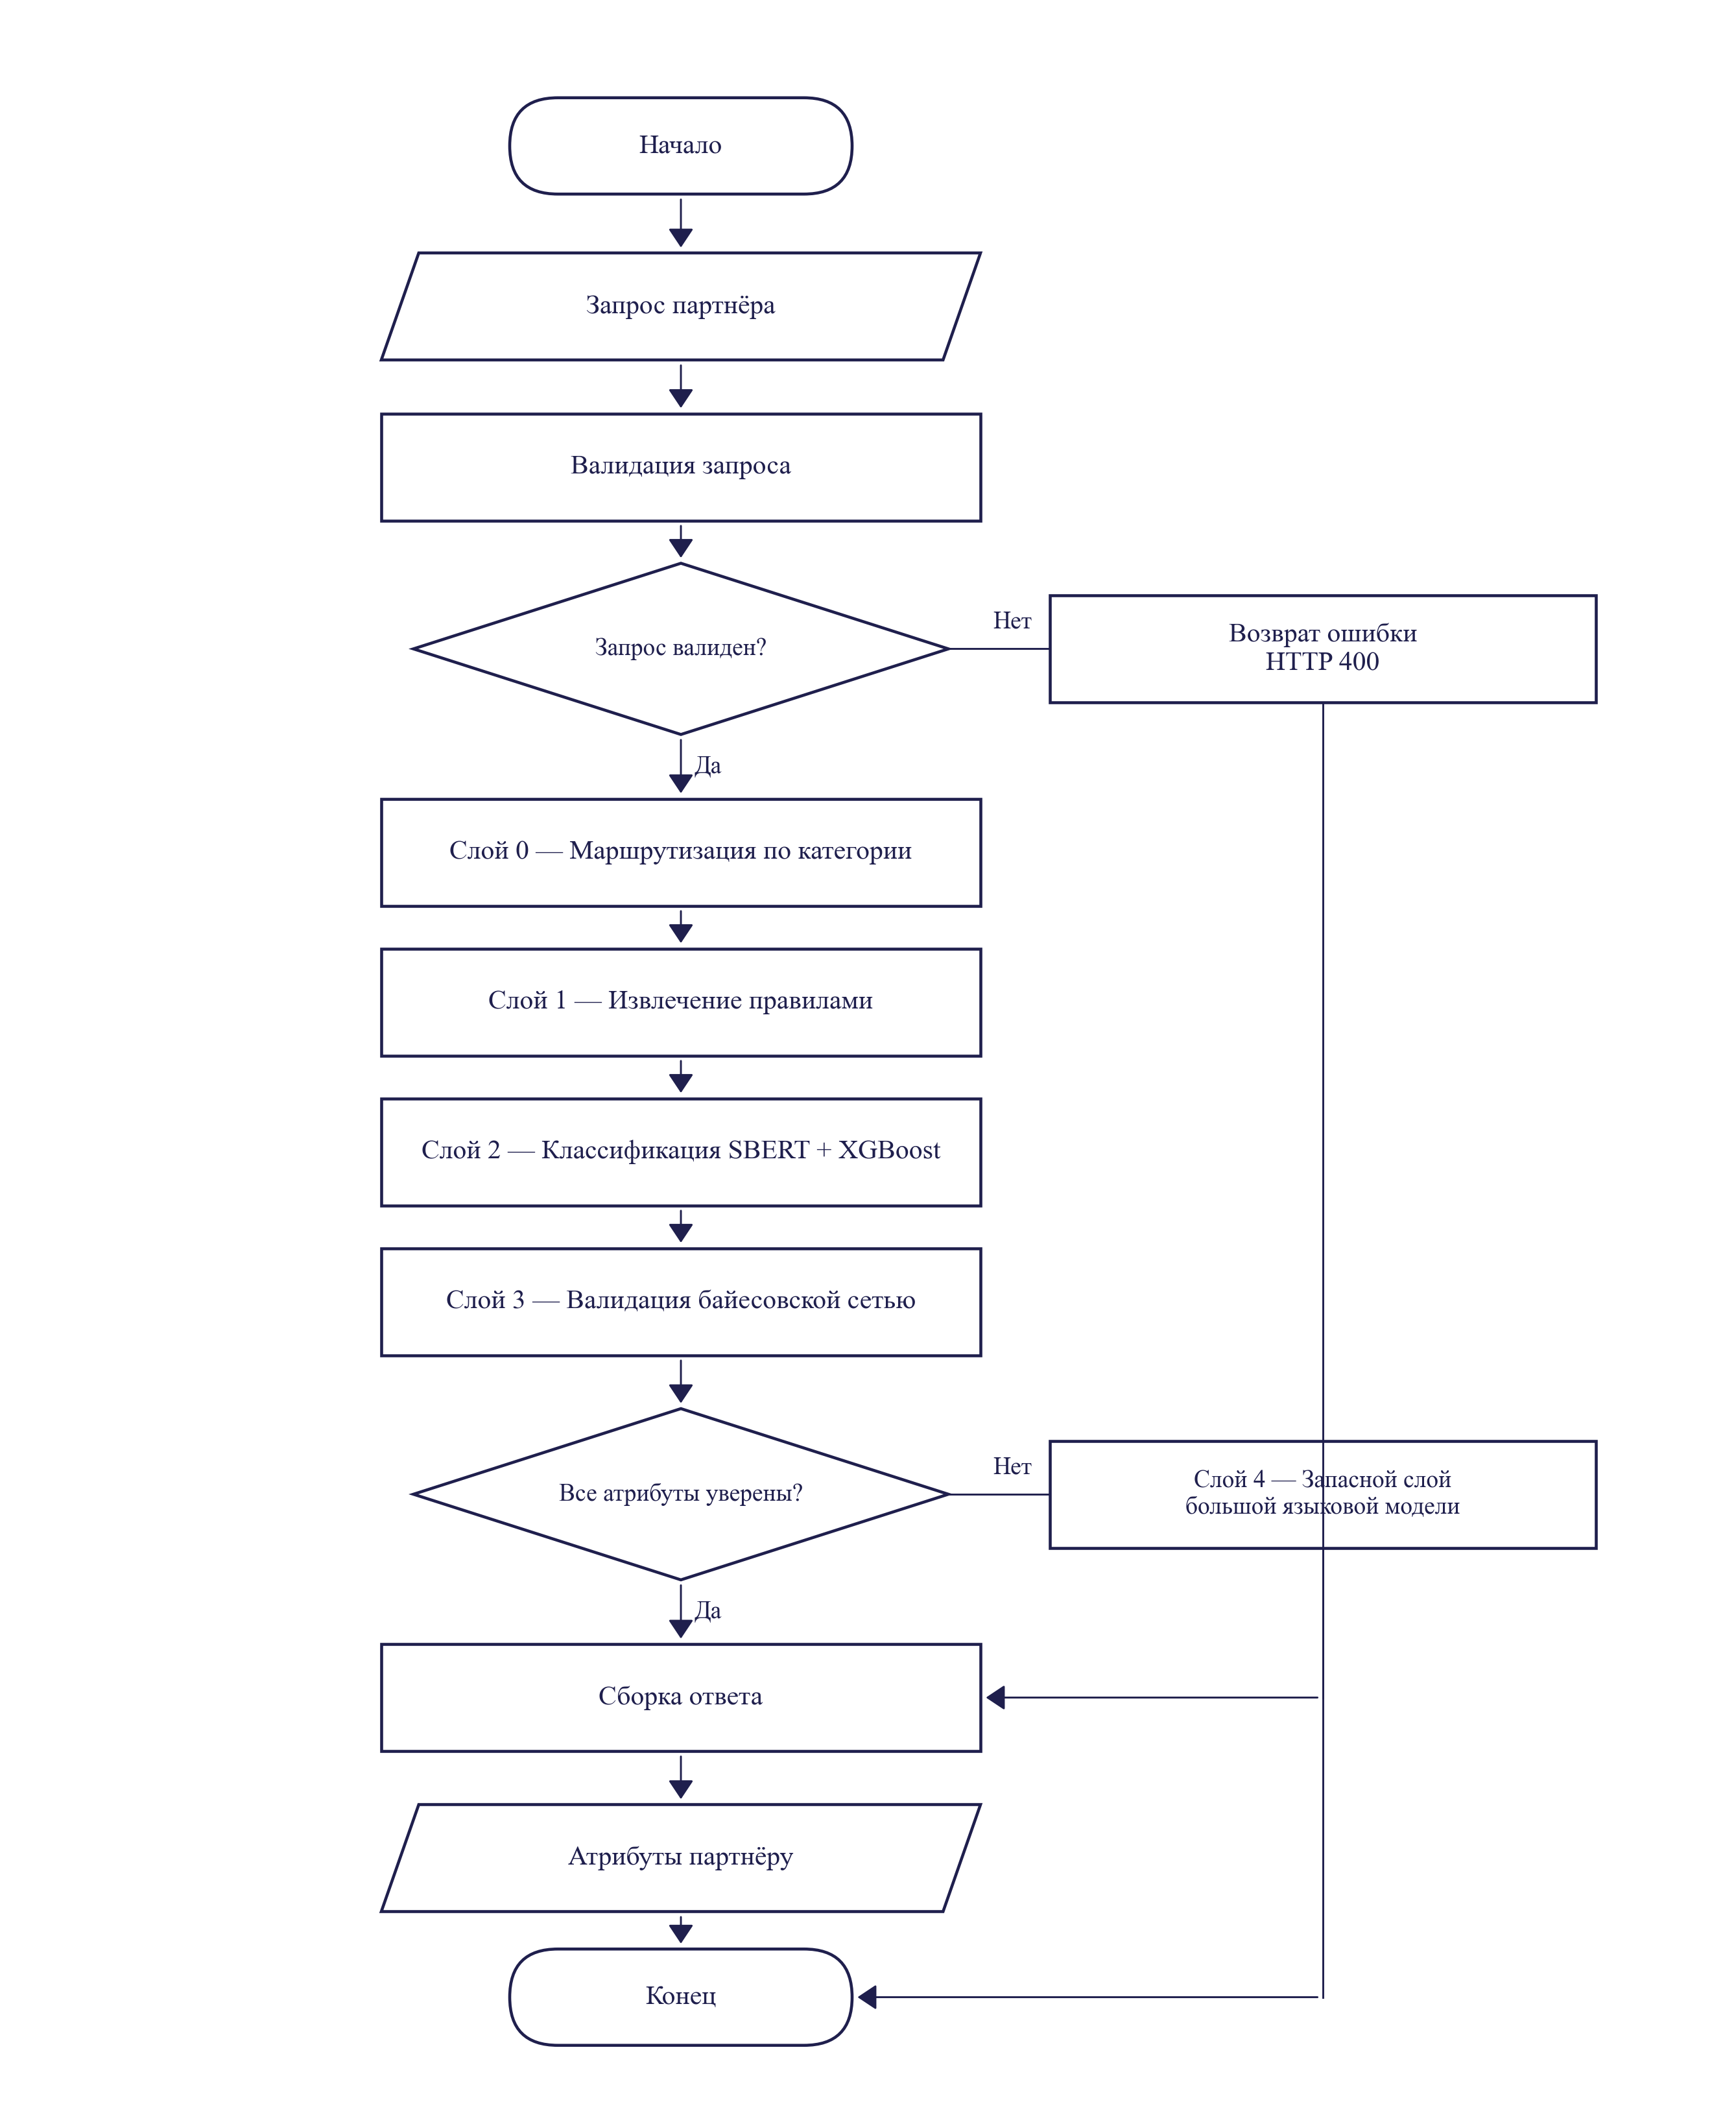
\includegraphics[width=\textwidth]{fig_3_1_algorithm_flowchart.png}
  \caption{Блок-схема алгоритма обработки запроса (нотация ГОСТ 19.701-90)}
  \label{fig:fig_3_1_algorithm_flowchart}
\end{figure}

\subsubsection{Демонстрационная система}

Трёхкомпонентная демонстрационная система имитирует встраивание в бизнес-процесс интернет-магазина.

\subsubsection{Архитектура компонентов}

Цепочка обработки: браузер (HTML/JS) → шлюз API на Go (\texttt{:8080}) → ML-сервис на Python/FastAPI (\texttt{:8001}) → каскад Слой 0 — regex — ML — Bayes — LLM.

Шлюз на Go (demo/gateway/, ≈200 строк, стандартная net/http) выполняет валидацию JSON, проксирование к ML-сервису, CORS, логирование и отдачу статического фронтенда. ML-сервис (demo/ml\_service/) при старте загружает SBERT-кодировщик, 24 XGBoost-классификатора, байесовские сети, словари порогов и слой 0; после прогрева (≈15–20 с) запросы к слоям 0–3 обрабатываются за десятки миллисекунд. Эндпоинты: \texttt{POST /api/enrich} (обогащение), \texttt{GET /api/categories} (схема), \texttt{GET /health} (готовность), \texttt{POST /api/explain} (Shapley-объяснения). Веб-интерфейс (demo/frontend/) — статическая HTML/JS-страница с формой ввода, переключателем категоризации, пресетами и блоком результата с отметкой слоя-источника.

\subsubsection{Контракт API}

Запрос \texttt{POST /api/enrich} принимает JSON с полями category (опционально; иначе сработает слой 0), product\_name, brands, ingredients\_text, quantity. Пример:

\begin{verbatim}
{ "category": "pasta", "product_name": "Spaghetti #5 Barilla",
  "brands": "Barilla", "ingredients_text": "Durum wheat semolina, water", "quantity": "500g" }
\end{verbatim}

Ответ содержит category, агрегированные счётчики (n\_attrs\_total, n\_covered, n\_llm\_fallback) и объект predictions, где для каждого атрибута указаны значение, слой-источник (regex / ml / llm\_fallback), уверенность и результат валидации:

\begin{verbatim}
{ "category": "pasta", "n_attrs_total": 8, "n_covered": 7, "n_llm_fallback": 1,
  "predictions": {
    "pasta_shape": { "value": "spaghetti", "layer": "regex", "confidence": 1.00 },
    "grain_type":  { "value": "wheat", "layer": "ml", "confidence": 0.99,
                     "validation": { "flagged": false, "p": 0.85, "threshold": 0.04 } },
    "is_filled":   { "value": null, "layer": "llm_fallback", "confidence": 0.0 } } }
\end{verbatim}

Явная отметка слоя-источника компенсирует ограниченную интерпретируемость слоёв 2/3 на уровне отдельного товара.

\subsubsection{Запуск и эксплуатация}

Запуск выполняется тремя командами (ML-сервис на \texttt{:8001}, Go-шлюз на \texttt{:8080}, браузер) либо одной — \texttt{bash reproduce.sh demo}. Готовность системы проверяется через \texttt{GET /health}. Стек технологий и обоснование компонентов — в 2.2.8 (таблица 2.1).

\subsection{Данные}

\subsubsection{Источник данных: Open Food Facts}

Основой выбран открытый каталог Open Food Facts (далее — OFF) — краудсорсинговая база ≈4,5 млн уникальных позиций под лицензией Open Database License (ODbL), допускающей коммерческое использование. Дамп получен командой \texttt{python -m src.data.download --source off} и конвертирован в parquet (\texttt{datasets/raw/en.openfoodfacts.org.products.parquet}, 526 МБ).

Выбор OFF обоснован тремя соображениями: открытость лицензии обеспечивает воспроизводимость; каталог репрезентативен и мультиязычен (50+ языков в product\_name и ingredients\_text); помимо текстовых полей OFF содержит структурированные нутриентные показатели (fat\_100g, sugars\_100g и др.) и регуляторные теги (labels\_tags, ingredients\_analysis\_tags), на которых построен эталон (3.2.3). Альтернативы (скрейпинг онлайн-магазинов, коммерческие PIM, теги Wikipedia) отклонены по лицензионным и покрытийным соображениям.

Область охвата — три категории: pasta, chocolate, cheeses. Они выбраны по критериям 1.3: достаточный объём, различие типа целевых атрибутов и наличие подгруппы атрибутов с детерминированным эталоном из нутриентов.

\subsubsection{Входные и целевые поля, фильтрация, стратифицированная выборка}

Поля OFF разделены на партнёр-доступные (product\_name, brands, quantity, ingredients\_text, code) и целевые выходные (categories\_tags, labels\_tags, \texttt{*\_100g}, ingredients\_analysis\_tags). Целевые поля не передаются на вход обучаемых компонентов под угрозой утечки; слой 2 формирует вход только из конкатенации \texttt{product\_name + brands + ingredients\_text + quantity}.

Фильтрация по категории (\texttt{src/data/filter.py}) использует списки включения/исключения categories\_tags (например, для pasta включение — \texttt{en:pastas}, \texttt{en:fresh-pastas}, исключение — \texttt{en:potato-products}, \texttt{en:rice-products}, \texttt{en:noodles}). После фильтрации применяется стратифицированная по языку выборка (определение языка — langdetect, страты — FR, EN, DE, IT, ES). Из каждой страты отбирается ≈250 товаров, итого ≈1250 на категорию (таблица 3.2.1).

\begin{xltabular}{\textwidth}{|X|X|X|X|}
\caption{Состав стратифицированной выборки по категориям, входящим в область охвата работы} \\ \hline
    Категория & Объём после фильтрации (сырые позиции) & Объём стратифицированной выборки & Число целевых атрибутов \\ \hline
\endfirsthead
\multicolumn{4}{l}{\textit{Продолжение таблицы}} \\ \hline
    Категория & Объём после фильтрации (сырые позиции) & Объём стратифицированной выборки & Число целевых атрибутов \\ \hline
\endhead
    pasta (макаронные изделия) & 15 691 & 1 250 & 8 \\ \hline
    chocolate (шоколад) & 13 469 & 1 250 & 7 \\ \hline
    cheeses (сыры) & 21 208 & 1 250 & 9 \\ \hline
\end{xltabular}

\textit{Примечание. Источник: \texttt{datasets/processed/\{cat\}\_stratified\_silver\_standard.parquet}.}

Целевые атрибуты определены в \texttt{src/pipeline/schemas/\{cat\}.py} и включают как кросс-категорийные (is\_organic, nutri\_score\_grade), так и специфичные (pasta\_shape, chocolate\_type, milk\_source, texture). Всего 24 пары (категория, атрибут) для 18 уникальных имён; экспериментальной оценке в 3.3 подлежат 22 пары (два атрибута cheeses — nutri\_score\_grade, protein\_class — обучены, но не оцениваются ввиду отсутствия соответствующей разметки в OFF).

\subsubsection{Эталонная разметка: иерархическая схема трёх ярусов}

Эталонная разметка построена как многоярусная процедура, где каждый ярус опирается на качественно различный класс свидетельств. Это даёт высокую точность при объёме, недостижимом для ручной разметки, и явно отделяет детерминированно разрешимые атрибуты от семантических.

Ярус 0 (нутриент-производные). Детерминированное бакетирование числовых полей: nutri\_score\_grade из \texttt{*\_100g} по регламенту ЕК 2017/1944, protein\_class из proteins\_100g, fat\_class из fat\_100g. Точность эталона — 100 \% при достоверных нутриентах, покрытие 95–100 \%.

Ярус 1 (тег-производные). Эталон из регуляторных тегов: is\_organic из \texttt{en:organic}, is\_gluten\_free из \texttt{en:gluten-free}, is\_pdo из \texttt{en:protected-designation-of-origin}. Достоверность опирается на правовую защиту меток в ЕС (регламенты 834/2007 и 1151/2012).

Ярус 2 (семантически-текстовые). Признаки без детерминированного правила: pasta\_shape, chocolate\_type, milk\_source, texture, contains\_nuts, cocoa\_percentage. Эталон — согласие трёх независимых LLM (Claude Sonnet 4.5, GPT-4o, Gemini 2.5 Flash) на полной выборке 1250 × 3 категории: атрибут принимается, если не менее двух моделей совпадают (согласованность 97,7 \%). Несогласованные позиции размечены слепо Claude Opus 4. Итог (\texttt{consensus\_gold\_v2\_expanded.parquet}) — 19 551 ячейка: 4 444 (ярус 0) + 7 108 (ярус 1) + 7 999 (ярус 2).

\subsubsection{Разбиение без пересечения брендов}

Случайное разбиение непригодно: бренд сам по себе сильный предиктор атрибутов (например, «Lindt» — тёмный шоколад определённого диапазона какао), и его попадание в обучение и тест одновременно завышает точность за счёт утечки. Эксплуатационный сценарий с регулярным подключением новых партнёров такая оценка не отражает.

Применяется разбиение без пересечения брендов (\texttt{src/data/split/brand\_disjoint.py}): уникальные бренды каждой категории делятся 60/20/20, все позиции бренда — в одно подмножество. Тест: 170 / 163 / 188 брендов в pasta / chocolate / cheeses; совокупно 1 423 / 1 270 / 1 657 = 4 350 ячеек (\texttt{headline\_v3e\_final.parquet}). Этот срез — основа всех количественных оценок 3.3.

\subsubsection{Дополнительные источники: разнородные модальности и внешний справочник}

Для усиления обучающего сигнала слоя 2 задействованы два дополнительных класса данных. Первый — разнородные модальности: фотографии этикеток обработаны OCR (EasyOCR); визуальный кодировщик CLIP \cite{ref_43} (ViT-B/32) даёт 512-мерный вектор, добавляемый ранней конкатенацией к 384-мерному SBERT-представлению. Покрытие изображениями ≈70 \%. Второй — внешний справочник USDA Branded Foods \cite{ref_44}, сопоставленный с выборкой приближённым поиском по \texttt{product\_name + brands} (Левенштейн, порог 0,85); даёт независимо измеренные нутриенты для проверки эталона яруса 0.

Оба источника используются только на этапе обучения. В режиме вывода система работает строго с партнёр-доступными полями (3.2.2); это инвариант, соблюдённый во всех оценках 3.3.

\subsection{Доказательство работоспособности и применимости}

\subsubsection{Условия проверки}

\subsubsection{Тестовая выборка}

Эксперименты проведены на единой тестовой выборке. Источник эталона — \texttt{consensus\_gold\_v2\_expanded.parquet} (схема ярусов — 3.2.3). Состав среза: 3 категории, 22 пары (категория, атрибут), 4350 ячеек после фильтрации непустых эталонных значений (234–239 кодов на категорию); уникальных брендов 170 / 163 / 188 (\texttt{headline\_v3e\_final.parquet}). Разбиение train/val/test без пересечения брендов выполнено в пропорции 60/20/20.

Независимая проверка эталона. Слепая разметка Claude Opus 4 без доступа к тегам OFF и промежуточным меткам проведена на 2666 кодах × 22 атрибута. Согласованность с эталоном — 95,0 \% на 4088 ненулевых ячейках (\texttt{blind\_vs\_prefill\_overall.parquet}); на 17 из 22 пар согласованность > 92 \%, κ Коэна > 0,85. Для трёх нутриент-производных пар Opus в слепом режиме отказывается отвечать в 82–93 \% случаев (правило бакетирования требует числовых полей); эталоном там выступает ярус 0.

\subsubsection{Метрики и доверительные интервалы}

Метрики ($\text{acc}^{\text{cov}}_k$, $\text{cov}_k$, $\text{acc}^{\text{e2e}}_k$, стоимость) определены в 2.1.4. Доверительные интервалы — кластерный бутстрэп по брендам: 1000 итераций, перцентили 2,5 \% и 97,5 \% (\texttt{src/diagnostics/ml/bootstrap\_ci\_brand\_clustered.py}). Такой интервал учитывает внутрибрендовую корреляцию ошибок и на ряде атрибутов на 15–30 \% шире наивного интервала Вильсона.

\subsubsection{Стратификация точности по типу эталонного сигнала}

Если бы точность завышалась структурной корреляцией признаков модели с источником эталона, то наиболее уязвимый ярус 2 (текстово-производный) показывал бы наибольшие значения. Результат обратный (таблица 3.3.1.1).

\begin{xltabular}{\textwidth}{|X|X|X|X|X|X|}
\caption{Точность каскада в разрезе типа эталонного сигнала} \\ \hline
    Ярус сигнала & Содержательная природа & Атрибутов & Ячеек & Точность, \% & 95 \% CI \\ \hline
\endfirsthead
\multicolumn{6}{l}{\textit{Продолжение таблицы}} \\ \hline
    Ярус сигнала & Содержательная природа & Атрибутов & Ячеек & Точность, \% & 95 \% CI \\ \hline
\endhead
    Ярус 0 (нутриент-производный) & Детерминированное бакетирование числовых полей OFF & 3 & 354 & 83,33 & [79,12; 87,20] \\ \hline
    Ярус 1 (тег-производный) & Регуляторные теги OFF, защищённые правом ЕС & 6 & 1 912 & 93,62 & [92,45; 94,69] \\ \hline
    Ярус 2 (текстово-производный) & Согласие трёх LLM с проверкой Opus 4 на спорных & 9 & 2 084 & 81,81 & [80,07; 83,61] \\ \hline
\end{xltabular}

\textit{Примечание. Источник: \texttt{datasets/processed/tier\_breakdown.parquet}.}

\begin{figure}
  
\includegraphics[width=\textwidth]{tier_breakdown.png}
  \caption{Точность каскада в разрезе ярусов эталонной разметки}
  \label{fig:tier_breakdown}
\end{figure}

Точность на ярусе 2 — наименьшая (81,8 \%, на 11,8 п. п. ниже яруса 1). На ярусе 1, где эталон порождён внешним источником (правовые регистры сертификаций), точность наиболее высокая (93,6 \%). Это опровергает гипотезу о завышении метрик за счёт зависимости признаков от эталона. На ярусе 0 показатель снижен парой cheeses/fat\_class (73,8 \%) — классификация жирности сыра объективно сложна.

\subsubsection{Воспроизводимость}

Все численные результаты 3.3 регенерируются из артефактов через \texttt{reproduce.sh} (≈час на типовом ноутбуке). Численные результаты 3.3.2 получены post-hoc после устранения утечки бренда и не претендуют на статус, фиксируемый до получения результатов. Единственной гипотезой, зафиксированной до получения результатов является H1 для обучаемого маршрутизатора (3.3.5).

\subsubsection{Главный результат: точность и стоимость производственной конфигурации}

Подраздел представляет центральный количественный результат: каскад сопоставлен с пятью одиночными вызовами LLM разной мощности и стоимости. На едином тестовом срезе без пересечения брендов показано доминирование каскада по Парето сразу по двум осям. Тем самым результат стоимостно-чувствительных каскадов LLM (FrugalGPT \cite{ref_9}, AutoMix \cite{ref_10}, Hybrid LLM \cite{ref_11}) расширяется на задачу обогащения каталогов; впервые количественно фиксируется выигрыш для открытой малой модели в роли запасного слоя.

\subsubsection{Состав, условия проверки и матрица «точность–стоимость»}

Оценка на 4350 ячейках без пересечения брендов (3.3.1); по атрибутам pasta/nutri\_score\_grade и pasta/protein\_class срез сокращён до 21 и 24 ячеек из-за полноты нутри-разметки в OFF. В роли слоя 4 и базовой «одна LLM на всё» — пять моделей: Claude Sonnet 4.5, GPT-4o, Gemini 2.5 Flash (закрытые), gpt-oss-120b и llama-3.2-3b (открытые).

Сводная таблица фиксирует сквозную точность и относительную стоимость десяти стратегий: пять одиночных LLM, пять каскадных конфигураций с теми же моделями и базовый каскад без LLM. Стоимость нормирована к «все ячейки решаются Sonnet 4.5»; соотношение токенов вход/выход — ≈500 / 200; тарифы — в подписи. Источник: \texttt{grand\_acc\_summary\_after\_fix.parquet}. Каскад покрывает 96,7 \% ячеек, LLM делается на 3,3 \% — множитель 0,033 относительно одиночной LLM.

\begin{xltabular}{\textwidth}{|X|X|X|X|}
\caption{Без подписи} \\ \hline
    Стратегия & Сквозная точность & Стоимость к опорной & Снижение стоимости \\ \hline
\endfirsthead
\multicolumn{4}{l}{\textit{Продолжение таблицы}} \\ \hline
    Стратегия & Сквозная точность & Стоимость к опорной & Снижение стоимости \\ \hline
\endhead
    all-sonnet (Claude Sonnet 4.5) — опорная конфигурация & 83,79 \% & 1,000 & 1× \\ \hline
    all-gpt-4o & 84,05 \% & 0,727 & 1,4× \\ \hline
    all-gemini-flash (Gemini 2.5 Flash) & 82,90 \% & 0,042 & 24× \\ \hline
    all-gpt-oss-120b (открытая модель) & 69,34 \% & 0,030 & 33× \\ \hline
    all-llama-3b (открытая малая модель) & 56,19 \% & 0,009 & 110× \\ \hline
    каскад + sonnet (Слой 4) & 92,78 \% & 0,033 & 30× \\ \hline
    каскад + gpt-4o & 92,90 \% & 0,024 & 42× \\ \hline
    каскад + gemini-flash & 92,78 \% & 0,0014 & 720× \\ \hline
    каскад + gpt-oss-120b & 92,32 \% & 0,0010 & 1007× \\ \hline
    каскад + llama-3b & 91,87 \% & 0,0003 & 3356× \\ \hline
    только каскад (без запасного слоя LLM) & 90,48 \% & 0,000 & — \\ \hline
\end{xltabular}

Источники тарифов: Sonnet 4.5 — 3 / 15 долларов за миллион токенов на вход / выход (нормализованная единица), GPT-4o — 2,5 / 10, Gemini 2.5 Flash — 0,075 / 0,30, gpt-oss-120b через OpenRouter — около 0,10 долларов за миллион токенов на запрос смешанной структуры, llama-3.2-3b через OpenRouter — около 0,03 долларов за миллион.

\begin{figure}
  
\includegraphics[width=\textwidth]{cost_quality_scatter.png}
  \caption{Матрица «точность — стоимость» каскадных конфигураций и одиночных вызовов больших языковых моделей}
  \label{fig:cost_quality_scatter}
\end{figure}

Из матрицы (рис. 3.3) следует двухчастный главный результат.

\textbf{Часть (а) — независимость от поставщика модели.} Каскад + Gemini 2.5 Flash даёт 92,78 \% при стоимости в 720 раз ниже all-sonnet (83,79 \%) — прирост +9,0 п. п. при снижении стоимости на два порядка; строгое Парето-доминирование. Результат сохраняется на любой модели верхнего сегмента: каскад + sonnet (92,78 \%) и каскад + gpt-4o (92,90 \%) также превосходят одиночный вызов той же модели по обеим осям.

\textbf{Часть (б) — сценарий локального развёртывания с открытой моделью.} Каскад + gpt-oss-120b — 92,32 \%, на +23,0 п. п. выше одиночного вызова (69,34 \%); доля обращений к LLM сокращается ≈в 30 раз. Каскад компенсирует слабость малой модели на нутриент-производных атрибутах (nutri\_score\_grade, protein\_class, fat\_class) за счёт Слой 2, оставляя слой 4 только сложные семантические случаи.

\subsubsection{Декомпозиция по категориям}

Покрытие каскада, точность только-каскадной и гибридной конфигураций и разность Δ — вклад запасного слоя — для модели gemini-flash в таблице 3.3.2.2. Источники: \texttt{headline\_v3e\_after\_fix.parquet} + \texttt{cascade\_plus\_llm4\_hybrid.parquet}; режим идеальной маршрутизации.

\begin{xltabular}{\textwidth}{|X|X|X|X|X|}
\caption{Покрытие и точность каскадной и гибридной конфигураций по категориям (модель gemini-flash, идеальная маршрутизация Слоя 0)} \\ \hline
    Категория & Покрытие каскада & Только каскад & каскад + gemini-flash & Δ от запасного слоя \\ \hline
\endfirsthead
\multicolumn{5}{l}{\textit{Продолжение таблицы}} \\ \hline
    Категория & Покрытие каскада & Только каскад & каскад + gemini-flash & Δ от запасного слоя \\ \hline
\endhead
    pasta & 97,1 \% & 93,3 \% & 95,8 \% & +2,5 п. п. \\ \hline
    chocolate & 96,4 \% & 87,4 \% & 90,1 \% & +2,7 п. п. \\ \hline
    cheeses & 96,6 \% & 90,4 \% & 92,2 \% & +1,8 п. п. \\ \hline
\end{xltabular}

Взвешенное по числу тестовых ячеек 1 423 / 1 270 / 1 657 среднее по строке «каскад + gemini-flash» составляет 92,78 \%. Производственное значение с учётом ошибок слоя 0 приблизительно на 2,4 п. п. ниже (3.3.2.5).

Распределение вклада запасного слоя вытекает из архитектуры. Pasta располагает наиболее развитым слоем 1: покрытие каскада 97,1 \%, на запасной слой передаются редкие случаи. Cheeses правил слоя 1 не имеет, ячейки покрывает слой 2 (96,6 \%), запасной слой берёт 3,4 \% самых сложных текстовых ячеек. Это показывает взаимодополнение слоёв.

\begin{figure}
  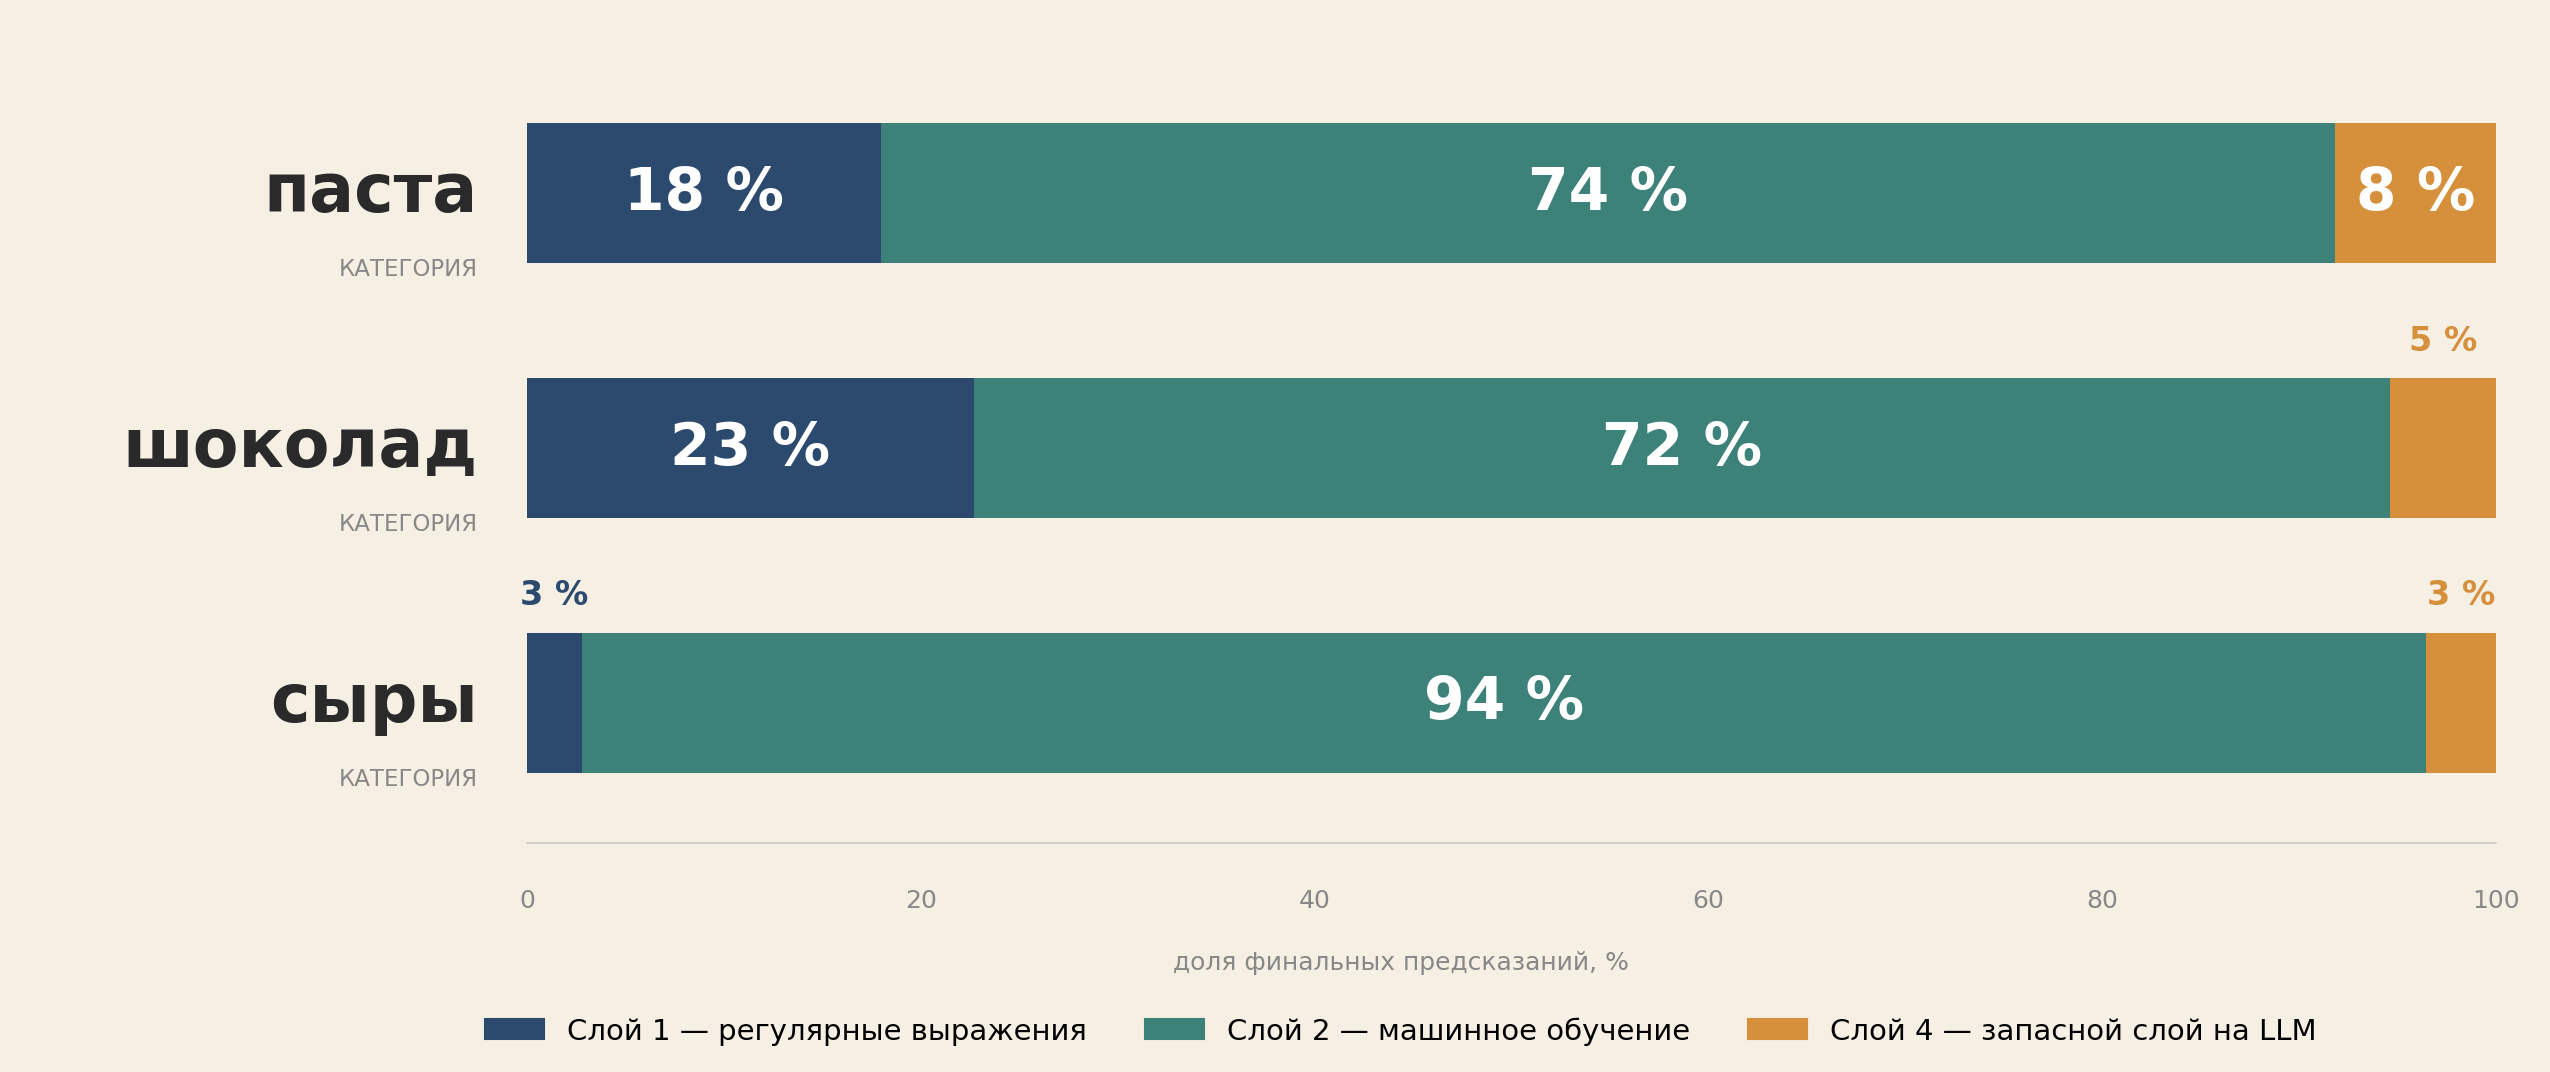
\includegraphics[width=\textwidth]{layer_contribution.png}
  \caption{Поатрибутный вклад слоёв каскада в сквозную точность}
  \label{fig:layer_contribution}
\end{figure}

\subsubsection{Поатрибутная картина точности и доверительные интервалы}

Для каждого из 22 атрибутов вычислена точность только-каскадной конфигурации с интервалом Вильсона (полная таблица — \texttt{headline\_v3e\_after\_fix.parquet}). Три лучших: cheeses/milk\_source 99,2 \% (n=238, [96,99; 99,77]), pasta/is\_filled 98,7 \% (n=239, [96,38; 99,57]), pasta/is\_gluten\_free 98,3 \% (n=239, [95,78; 99,35]). Три худших: chocolate/protein\_class 52,4 \% (n=42, [37,72; 66,64]), cheeses/fat\_class 63,6 \% (n=225, [57,09; 69,57]), pasta/protein\_class 66,7 \% (n=24, [46,71; 82,03]).

В 3.3.7.4 описаны поатрибутные архитектурные решения (сужение слоя 1, понижение порогов слоя 2, гибридные признаки). Запасной слой остаётся доступным на ≈3 \% сложных ячеек, где Слой 1/2 не отвечают уверенно: pasta/protein\_class, chocolate/protein\_class, cheeses/fat\_class.

\subsubsection{Анализ доминирования по Парето: почему каскад превосходит одиночный вызов LLM}

Доминирование каскада объясняется структурно. LLM системно проигрывает на производных числовых атрибутах: точность Sonnet 4.5 на chocolate/cocoa\_percentage — 67,2 \%, на cheeses/fat\_class — 26,2 \% (\texttt{cascade\_plus\_llm4\_hybrid.parquet}). Причина — метки этих атрибутов определяются бакетированием числовых полей, которых в тексте нет. XGBoost слоя 2 на SBERT-эмбеддингах опирается на устойчивые корреляции «бренд — числовое поле». Точность каскада растёт за счёт перенаправления таких атрибутов на ML-слой; стоимость падает за счёт сокращения вызовов LLM до 3,3 \% ячеек.

\subsubsection{Учёт точности маршрутизатора первого уровня}

Значения рисунка 3.4 — в режиме идеальной маршрутизации. В производстве категорию определяет слой 0 (3.1.1) с точностью 96,3 \% / 98,5 \% / 97,7 \% по категориям (\texttt{cascade\_layer0\_eval.parquet}). С учётом ошибок слоя 0 заголовочная точность 92,78 \% понижается ≈на 2,4 п. п. равномерно по всем строкам; вывод о доминировании каскада сохраняется.

\subsubsection{Вклад каждого слоя каскада}

Подраздел декомпозирует итоговую точность по слоям: охват, точность на собственном срезе и средняя калибровочная ошибка ECE для слоя 2. Артефакты — \texttt{cascade\_preds\_\{pasta,chocolate,cheeses\}\_v2\_gold\_hybrid\_v3\_fixed.parquet}, \texttt{headline\_v3e\_final.parquet}, \texttt{ece\_calibration\_table.parquet}.

\subsubsection{Распределение закрытий по слоям}

Закрытие — событие выдачи уверенного ответа без передачи дальше. Доли по слоям (колонка layer в \texttt{cascade\_preds\_*}) — таблица 3.3.3.1. Подсчёт ведётся по всем 24 парам (см. 3.2.2); суммарно 5258 ячеек (больше 4350 из 3.3.1, где отбрасываются непустые эталоны по 22 парам).

\begin{xltabular}{\textwidth}{|X|X|X|X|X|}
\caption{Без подписи} \\ \hline
    Категория & Слой 1 (regex) & Слой 2 (ML) & Отказ (передача на слой 4) & Всего ячеек \\ \hline
\endfirsthead
\multicolumn{5}{l}{\textit{Продолжение таблицы}} \\ \hline
    Категория & Слой 1 (regex) & Слой 2 (ML) & Отказ (передача на слой 4) & Всего ячеек \\ \hline
\endhead
    pasta & 18,0 \% (344) & 73,8 \% (1412) & 8,2 \% (156) & 1912 \\ \hline
    chocolate & 22,7 \% (380) & 71,9 \% (1203) & 5,4 \% (90) & 1673 \\ \hline
    cheeses & 2,8 \% (47) & 93,7 \% (1567) & 3,5 \% (59) & 1673 \\ \hline
\end{xltabular}

Распределение неоднородно: pasta и chocolate располагают наиболее полным набором правил (18,0 \% и 22,7 \% закрытий на слой 1 соответственно); cheeses имеет узкий набор правил (milk\_source / is\_pdo / is\_ultra\_processed) с покрытием 2,8 \%, что отражает плохую параметризуемость доменных сигналов сыра (текстура, страна происхождения, класс жирности) регулярными выражениями — эти атрибуты переданы на ML-слой.

\subsubsection{Точность каждого слоя на собственном срезе закрытий}

Точность получена сопоставлением \texttt{cascade\_preds\_*} с \texttt{consensus\_gold\_v2\_expanded.parquet} (только ненулевые эталоны).

\begin{xltabular}{\textwidth}{|X|X|X|}
\caption{Без подписи} \\ \hline
    Категория & Слой 1: точность (n) & Слой 2: точность (n) \\ \hline
\endfirsthead
\multicolumn{3}{l}{\textit{Продолжение таблицы}} \\ \hline
    Категория & Слой 1: точность (n) & Слой 2: точность (n) \\ \hline
\endhead
    pasta & 90,5 \% (327) & 98,6 \% (1035) \\ \hline
    chocolate & 87,0 \% (370) & 94,9 \% (802) \\ \hline
    cheeses & 100,0 \% (47) & 93,5 \% (1549) \\ \hline
\end{xltabular}

Точность слоя 1 на закрытых ячейках 87,0–90,5 \% (ниже 100 \% из-за намеренно широких regex-шаблонов и пограничных значений при бакетировании cocoa\_percentage). Точность слоя 2 — 94,9–98,6 \%; стабильно выше любого одиночного вызова LLM на той же категории, так как слой работает только на ячейках, прошедших калиброванный порог.

Точность запасного слоя на отказных ячейках оценена через поатрибутную точность LLM, взвешенную по числу отказных ячеек (формула acc\_hybrid\_proxy в \texttt{cascade\_plus\_llm4\_hybrid.parquet}): Gemini 2.5 Flash — 78,8 \%, Claude Sonnet 4.5 — 76,7 \%, gpt-oss-120b — 67,2 \%. Эти значения ниже слоёв 1/2 и отражают повышенную сложность отказных ячеек.

\subsubsection{Поатрибутная калибровочная ошибка до и после калибровки}

Поатрибутная ожидаемая калибровочная ошибка (ECE) рассчитана по 10 равновеликим бинам (\texttt{ece\_calibration\_table.parquet}). Среднее ECE сырого XGBoost — 0,070 (по 22 замерам); у большинства атрибутов не превосходит 0,08. Повышенная ошибка: cheeses/fat\_class (0,22), chocolate/chocolate\_type (0,14), chocolate/protein\_class (0,11).

Изотоническая пост-калибровка на серебряной выборке локально улучшает проблемные атрибуты (chocolate/chocolate\_type −7,8 п. п., cheeses/fat\_class −6,0 п. п.), но в среднем по 20 атрибутам ECE ухудшается на +0,012 за счёт деградации на других (chocolate/cocoa\_percentage: −26,0 п. п.). Эффект объясняется дрейфом разметки между серебряной (теги OFF) и эталонной (консенсус LLM) выборками.

Для устранения дрейфа проведена изотоническая калибровка на распределении эталонной выборки по схеме 5-кратной перекрёстной валидации: на каждом фолде отображение строится на 4 частях и оценивается на отложенной (\texttt{ece\_kfold\_gold\_table.parquet}, \texttt{src/diagnostics/ml/ece\_kfold\_gold.py}). Среднее ECE падает с 0,070 до 0,043 (−2,78 п. п. в среднем), положительный эффект на 18 из 22 атрибутов. Наибольшие улучшения концентрируются на парах с высокой исходной ошибкой: cheeses/fat\_class (0,220 → 0,075, −14,5 п. п.), chocolate/chocolate\_type (0,139 → 0,052, −8,7 п. п.), chocolate/protein\_class (0,111 → 0,041, −7,0 п. п.), pasta/is\_organic (0,084 → 0,016, −6,9 п. п.). Ухудшение — у четырёх атрибутов с изначально низкой ECE: cheeses/country\_of\_origin (0,015 → 0,064), cheeses/is\_ultra\_processed (0,025 → 0,056), pasta/pasta\_shape (0,046 → 0,060), chocolate/contains\_nuts (0,055 → 0,058); здесь доминируют выборочные колебания. В производственную конфигурацию калибровка пока не включена (см. раздел «Перспективы развития темы» заключения).

Итог: Слой 1 закрывает 2,8–22,7 \% ячеек (точность 87,0–100 \% в зависимости от категории и шаблона); Слой 2 — 71,9–93,7 \% (93,5–98,6 \%); Слой 4 — 3,5–8,2 \% (67,2–78,8 \% в зависимости от модели). Среднее ECE по слою 2 — 0,070; серебряная пост-калибровка устойчивого эффекта не даёт.

\subsubsection{Обоснование сохранения слоя регулярных выражений: сопоставление с обучаемыми альтернативами}

Использование детерминированных правил в качестве слоя 1 — нетривиальный выбор, требующий ручной разработки для каждой категории. Для его количественной фиксации каскад с regex сопоставлен с восемью альтернативами, где слой 1 заменён обучаемой моделью (\texttt{src/experiments/layer1\_5\_*.py}, \texttt{src/experiments/lexicon\_regex.py}; артефакты — \texttt{layer1\_5\_optimal.parquet}, \texttt{lexicon\_regex\_comparison.parquet}). Все варианты оценены на едином 80/20-разбиении (seed = 42) по 22 парам.

\begin{xltabular}{\textwidth}{|X|X|X|X|}
\caption{Сопоставление каскадных конфигураций с разным первым слоем} \\ \hline
    Вариант & Состав первого слоя (перед основным ML-слоем) & Средняя точность & Δ к «без первого слоя» \\ \hline
\endfirsthead
\multicolumn{4}{l}{\textit{Продолжение таблицы}} \\ \hline
    Вариант & Состав первого слоя (перед основным ML-слоем) & Средняя точность & Δ к «без первого слоя» \\ \hline
\endhead
    A & Регулярные выражения (текущая конфигурация) & 83,58 \% & +1,38 п. п. \\ \hline
    B & Без первого слоя (один ML-слой) & 82,20 \% & 0 \\ \hline
    C & Наивный байесовский классификатор на n-граммах & 82,16 \% & −0,04 \\ \hline
    D & Решающее дерево & 82,98 \% & +0,78 \\ \hline
    E & Центроидный классификатор в пространстве n-грамм & 82,22 \% & +0,02 \\ \hline
    F & Логистическая регрессия на n-граммах & 82,23 \% & +0,03 \\ \hline
    L & Обучаемый словарь n-грамм (lexicon) & 83,00 \% & +0,80 \\ \hline
    G & Поатрибутный выбор лучшего метода по перекрёстной проверке & 81,99 \% & −0,21 \\ \hline
    H & Регулярные выражения — решающее дерево — ML (последовательно) & 83,78 \% & +1,58 \\ \hline
\end{xltabular}

Источник — \texttt{docs/layer1\_5\_optimal\_recommendation.md}. Из таблицы следуют три вывода.

Во-первых, чистый ML без слоя 1 (B, 82,20 \%) уступает текущей конфигурации (A, 83,58 \%) на 1,38 п. п. — regex даёт небольшой, но устойчивый прирост.

Во-вторых, ни одна обучаемая альтернатива (C, D, E, F, L) не превосходит regex в роли единственного слоя 1. Регулярные правила формализуют доменное знание (формы пасты, типы зерна, числовые шаблоны какао), не восстанавливаемое из распределения слов: лексические маркеры редки, но однозначны.

В-третьих, единственная статистически превосходящая regex конфигурация — композиция «regex — дерево — ML» (H, +0,20 п. п.). Прирост незначителен и не оправдывает усложнения и поддержки 22 деревьев.

Таким образом, выбор regex как Слой 1 эмпирически обоснован: наибольший прирост среди простых альтернатив при детерминированном выводе и отсутствии переобучения. Предпочтительное развитие — точечное расширение правил по итогам 3.3.7.4.

\subsubsection{Поведение байесовского валидатора}

\subsubsection{Постановка задачи и калибровка порога}

Слой 3 — байесовская сеть над дискретизированными атрибутами и брендом. Структура сети обучается алгоритмом Hill Climb с критерием BIC; пример полученного направленного ациклического графа для категории chocolate приведён на рисунке 3.5. Эмпирически роль классификатора неэффективна (точность ≈52 \%, ниже мажорной точки отсчёта), поэтому сеть применяется как валидатор плотности: для предсказания слоя 2 вычисляется $P(\text{value}\mid\text{evidence})$ при свидетельствах «бренд + остальные атрибуты». Ниже порога — ячейка помечается и передаётся в Слой 4. Порог индивидуален для каждой пары и фиксируется на этапе обучения как 5-перцентиль распределения $P$ на обучающей выборке.

\begin{figure}
  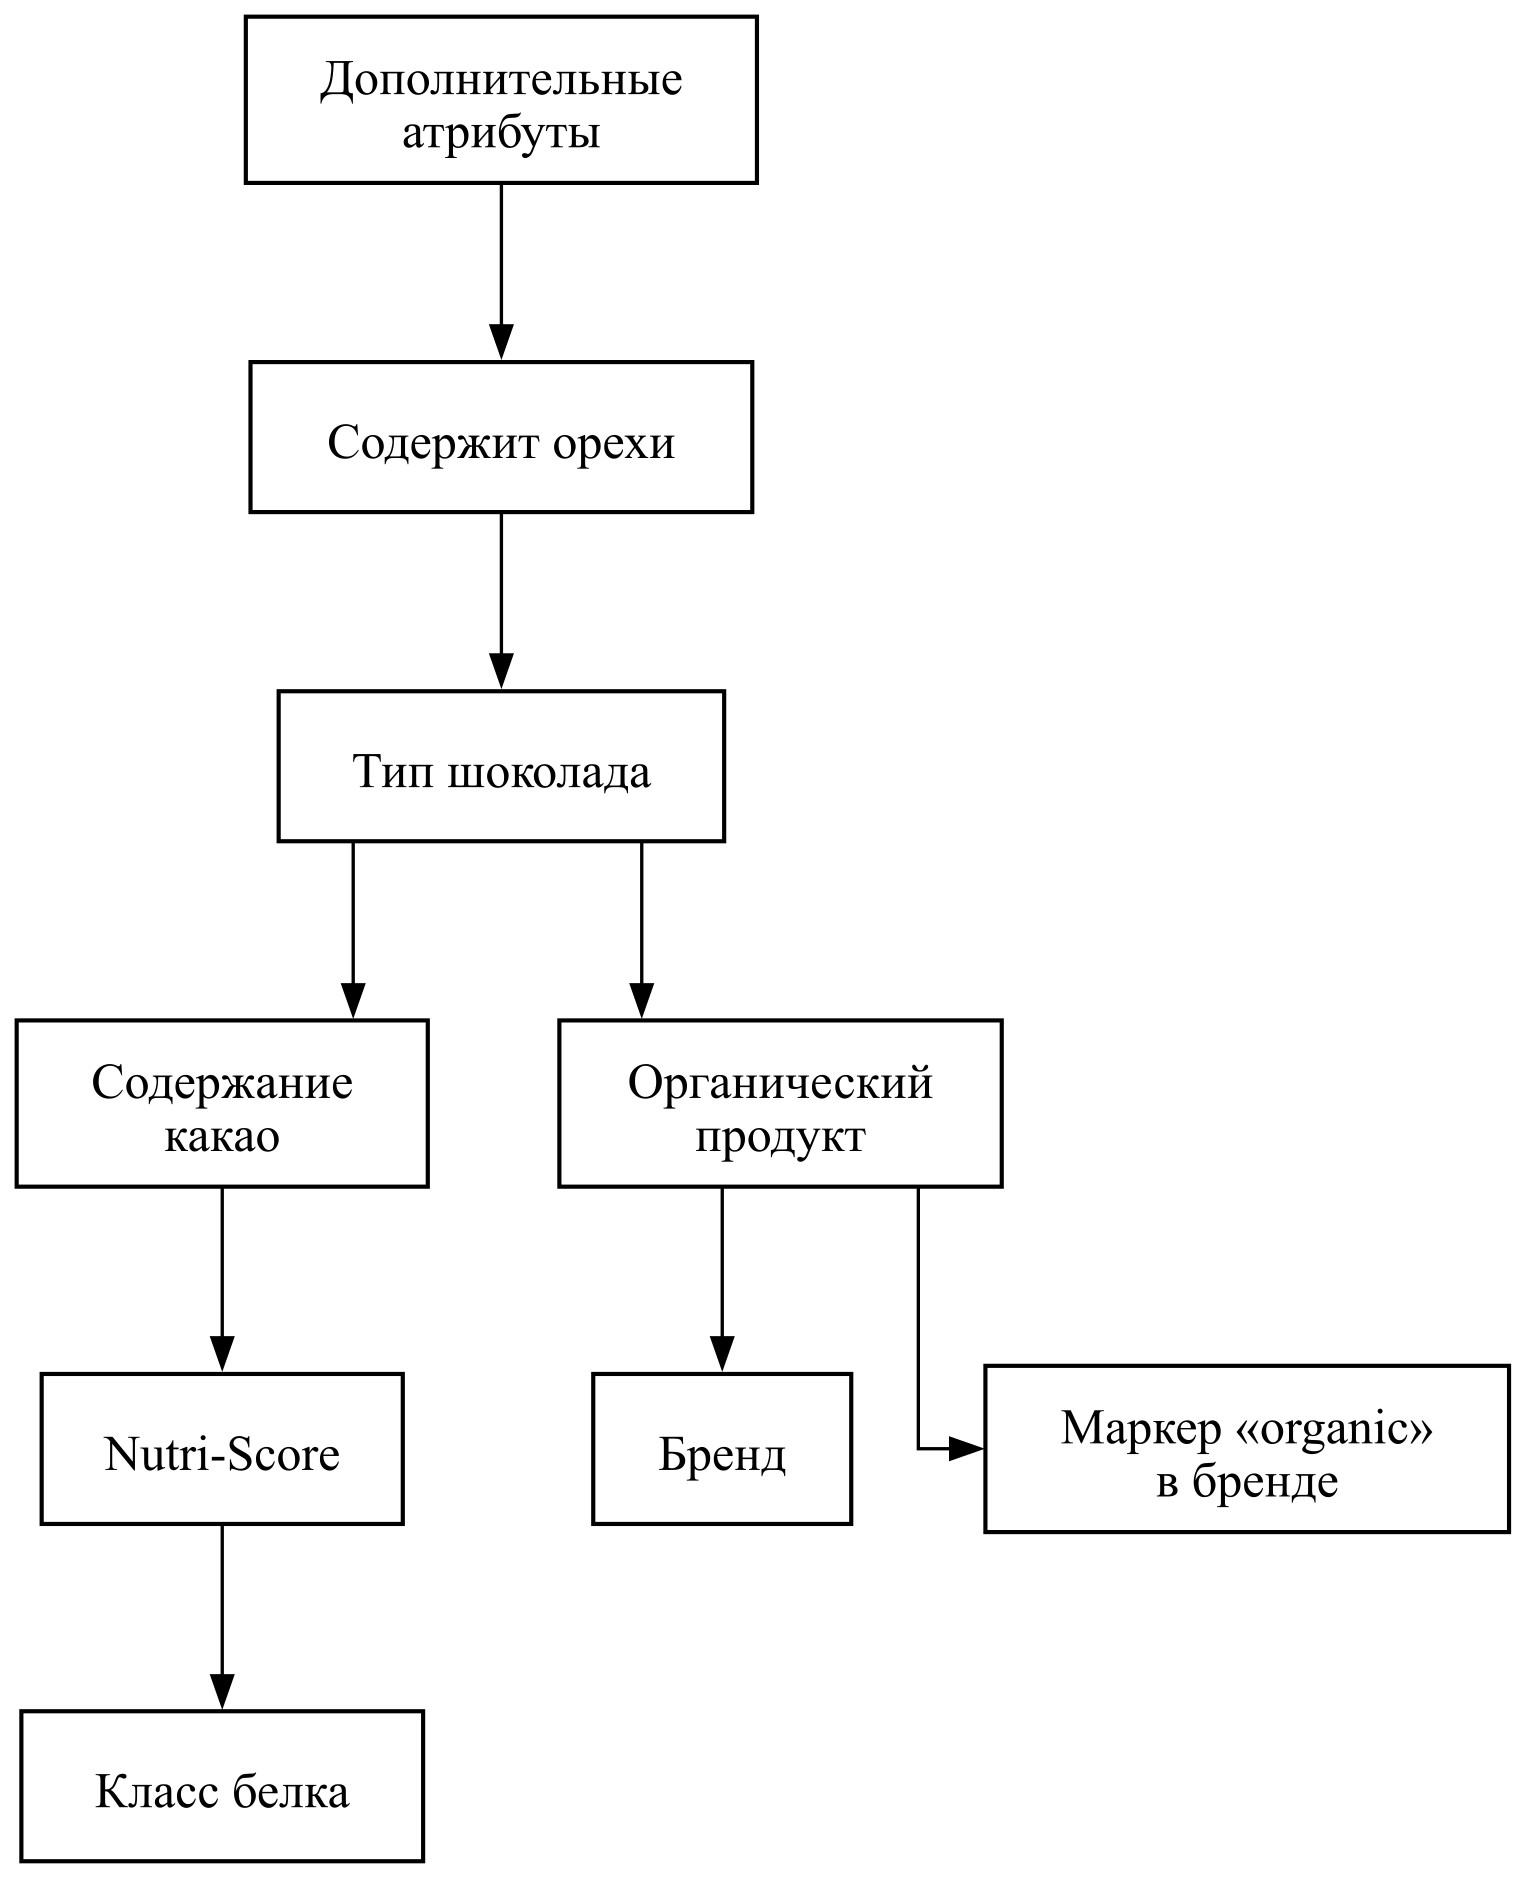
\includegraphics[width=\textwidth]{fig_3_5_bayes_dag.png}
  \caption{Структура байесовской сети категории chocolate (направленный ациклический граф, обученный алгоритмом Hill Climb с критерием BIC)}
  \label{fig:fig_3_5_bayes_dag}
\end{figure}

Агрегированные результаты по трём категориям приведены в таблице 3.3.4.1 (\texttt{bayes\_validator\_demote\_metric.parquet}).

\begin{xltabular}{\textwidth}{|X|X|X|X|X|X|X|X|}
\caption{Поведение байесовского валидатора на категориях pasta, chocolate, cheeses} \\ \hline
    Категория & n\_ml & Доля помеченных & Точность каскада & Точность отбраковки & Базовая точка отсчёта & Прирост & Полнота \\ \hline
\endfirsthead
\multicolumn{8}{l}{\textit{Продолжение таблицы}} \\ \hline
    Категория & n\_ml & Доля помеченных & Точность каскада & Точность отбраковки & Базовая точка отсчёта & Прирост & Полнота \\ \hline
\endhead
    pasta & 1010 & 7,9 \% & 98,6 \% & 2,5 \% & 1,4 \% & +1,1 п. п. & 14,3 \% \\ \hline
    chocolate & 772 & 14,1 \% & 94,7 \% & 20,2 \% & 5,3 \% & +14,9 п. п. & 53,7 \% \\ \hline
    cheeses & 1436 & 6,1 \% & 96,3 \% & 1,1 \% & 3,7 \% & −2,5 п. п. & 1,9 \% \\ \hline
\end{xltabular}

Калибровка работает на pasta и cheeses (7,9 \% и 6,1 \% помеченных при целевом 5 \%). На chocolate доля 14,1 \%, почти втрое выше: отклонение объясняется смещением маржинального распределения contains\_nuts на тестовых брендах относительно серебряной выборки калибровки (согласуется с 3.3.7).

\subsubsection{Метрика отбраковки и селективность сигнала}

Точность отбраковки — $\text{TP}/(\text{TP}+\text{FP})$ среди помеченных. Базовая точка отсчёта — частота ошибок каскада на всех ячейках пары. Прирост — разность; положительный прирост означает, что валидатор обогащает отправляемую в LLM выборку реальными ошибками. Полнота — $\text{TP}/(\text{TP}+\text{FN})$.

Из 22 пар лишь три демонстрируют точность отбраковки выше базовой:

\begin{itemize}
    \item chocolate / contains\_nuts: точность отбраковки 53,7 \% при базовой точке отсчёта 15,5 \%, прирост +38,2 п. п., полнота отбраковки 59,5 \%;
    \item pasta / is\_vegan: точность отбраковки 20,0 \% при базовой точке отсчёта 6,0 \%, прирост +14,0 п. п. (n\_flagged = 10);
    \item cheeses / is\_pdo: точность отбраковки 10,0 \% при базовой точке отсчёта 3,0 \%, прирост +7,0 п. п. (n\_flagged = 10).
\end{itemize}

Для оставшихся 19 пар точность отбраковки базовую точку отсчёта не превышает. Эффект валидатора локализован: он не является универсальным фильтром, равномерно повышающим качество всех помеченных ячеек.

\subsubsection{Бизнес-эффект и архитектурный вывод}

При сплошном понижении (все помеченные ячейки в LLM) средняя точность каскада снижается на 0,4 п. п. при росте расходов на LLM на 8,6 п. п. — чистый эффект отрицателен: ложные срабатывания на 19 пар размывают сигнал трёх работающих. При точечном понижении на паре chocolate/contains\_nuts точность категории chocolate растёт на 6,6 п. п. при росте расходов на 5,3 п. п. Этот режим включён в финальную конфигурацию.

Перевод сети из роли классификатора в роль валидатора плотностей иллюстрирует общий принцип: невостребованный в одной роли компонент может с пользой вернуться в систему через изменение роли. Совмещение точечного валидатора с архитектурными решениями 3.3.7.4 даёт chocolate/contains\_nuts 91,2 \% сквозной точности (\texttt{headline\_v3e\_after\_fix.parquet}).

\subsubsection{Стоимостно-чувствительный маршрутизатор: отрицательный результат}

\subsubsection{Идея, гипотеза H1 и процедура оценки}

Финальный механизм направления ячеек в LLM — статическое per-(категория, атрибут) правило. На этапе проектирования рассматривалась обучаемая альтернатива: XGBoost-маршрутизатор предсказывает надёжность ответа каскада на каждой ячейке; при вероятности ниже τ ячейка идёт в LLM. \textbf{Гипотеза H1:} при равном бюджете LLM обучаемый маршрутизатор обеспечивает более высокую точность, чем статическое правило. H0: разница незначима.

Оценка проведена по процедуре, зафиксированной до получения результатов. До доступа к числам зафиксированы: три бюджета LLM (25 \%, 40 \%, 50 \%); поправка Бонферрони на три теста (α/3 ≈ 0,0167 при α = 0,05); тестовая выборка без пересечения брендов (n = 1539); опорная конфигурация — статическое правило. Все параметры зафиксированы в \texttt{src/eval/router\_pre\_registered.py} (константы \texttt{PRE\_REGISTERED\_BUDGETS}, BONFERRONI\_N, функция evaluate\_h1). Коммит модуля (\texttt{cd9ac7a}, 2026-05-13 02:11) сделан за 1 ч 11 мин до создания артефакта \texttt{router\_pareto\_gold.parquet} (03:22 того же дня), что фиксирует временной приоритет процедуры над данными.

Гипотеза H1 зафиксирована в git-коммите \texttt{cd9ac7a} от 2026-05-13 до получения окончательных результатов оценки без пересечения брендов. Платформа предварительной регистрации (OSF, AsPredicted) не использовалась; фиксация через коммит репозитория обеспечивает воспроизводимость и временной приоритет, но не равна третьесторонней публикации протокола.

\subsubsection{Результаты}

Сравнительные числа на выборке без пересечения брендов представлены в таблице 3.3.5.1 (\texttt{router\_pareto\_gold.parquet}; для пяти моделей запасного слоя — \texttt{router\_pareto\_gold\_\{model\}.parquet}).

\begin{xltabular}{\textwidth}{|X|X|X|X|}
\caption{Сравнение конфигураций маршрутизации на проверочной выборке без пересечения брендов} \\ \hline
    Конфигурация & Точность & Доля вызовов LLM & Тип \\ \hline
\endfirsthead
\multicolumn{4}{l}{\textit{Продолжение таблицы}} \\ \hline
    Конфигурация & Точность & Доля вызовов LLM & Тип \\ \hline
\endhead
    Только каскад (без LLM) & 78,5 \% & 0 \% & опорная конфигурация \\ \hline
    Статический порог τ = 0,55 & 82,6 \% & 11 \% & статический \\ \hline
    Обучаемый маршрутизатор (оптимум) & 82,7 \% & 16 \% & обучаемый \\ \hline
    Статическое поатрибутное правило & 83,9 \% & 58 \% & статический \\ \hline
\end{xltabular}

Приведены точки минимальной стоимости при сопоставимой точности. Проверка H1 — сравнение точностей при равных бюджетах 25 \%, 40 \%, 50 \%. При сопоставимой точности обучаемый маршрутизатор требует более высокого бюджета LLM: 16 \% против 11 \% при разнице точностей 0,1 п. п. в пределах доверительного интервала (n = 1 539).

Ни на одном из трёх бюджетов маршрутизатор не превзошёл опорную конфигурацию на уровне α/3 после поправки Бонферрони. Гипотеза H1 отклонена.

При n = 1539, скорректированном уровне значимости α/3 ≈ 0,0167 (поправка Бонферрони на три бюджетных режима) и целевой мощности 0,8 минимальный обнаруживаемый эффект (MDE) для парного теста составляет ≈ \textbf{4,4 п. п.} (нормальная аппроксимация при средней точности конфигураций p ≈ 0,83; точный McNemar-тест по симуляции даёт более оптимистичную оценку ≈ 3,0 п. п. при типичной доле discordant-пар 10 \%). Отрицательный исход H1 при таком размере выборки следует интерпретировать как отсутствие практически значимого превосходства обучаемого маршрутизатора над статическим правилом в пределах не менее 4 п. п.; меньшие сдвиги настоящей оценкой не отвергаются и не подтверждаются.

\subsubsection{Интерпретация и следствие для финальной конфигурации}

Отклонение H1 воспроизводится на всех пяти моделях Слой 4 и объясняется тремя наблюдениями. Во-первых, основная вариация надёжности каскада сосредоточена на уровне атрибутов, а не товаров; статическое per-(категория, атрибут) правило учитывает именно эту неоднородность, маршрутизатор уровня ячейки дополнительной информации не привносит. Во-вторых, выборка без пересечения брендов устраняет утечку бренда, объяснявшую ранние положительные результаты на случайных разбиениях. В-третьих, результат согласуется с RouterBench \cite{ref_12}: обучаемый маршрутизатор не доминирует над простыми правилами при локализованной структуре ошибок.

В финальной конфигурации применяется статическое правило: оно прозрачно, поддаётся аудиту и не требует переобучения. Отклонение H1 — один из трёх пунктов научной новизны работы (см. введение).

\subsubsection{Цикл «аудит — правки экстрактора — переобучение — измерение»}

Замкнутый цикл итеративного улучшения каскада построен на сопоставлении собственных предсказаний с независимо проаудированной разметкой. Измерение по неизменному списку аудированных ячеек исключает селекционный сдвиг.

\subsubsection{Аудит pasta}

Для pasta сформирован эталонный набор из 239 продуктов; LLM-аудитор \texttt{anthropic/claude-opus-4} слепо вынес суждения по каждой ячейке. Артефакт \texttt{cascade\_vs\_audited\_gold\_pasta.json} — 1841 ячейка по 8 атрибутам; доля override + manual\_only — 220/1841 (11,95 \%).

Главное обнаружение — концентрация ошибок на одном атрибуте: 24,2 \% значений pasta\_shape ошибочны. Корень — функция \texttt{\_type\_b\_multiclass} обходила categories\_tags в порядке следования, а не приоритета специфичности: для итальянской, испанской и немецкой пасты обобщённый \texttt{en:noodles} опережал специфические \texttt{en:tagliatelle}, \texttt{en:penne}, \texttt{en:fusilli}. Дополнительно: TYPE\_B не содержала legume-pasta и filled-pasta, regex не знал многоязычные синонимы форм.

\subsubsection{Правки экстрактора}

Внесены точечные правки (коммиты \texttt{c1a0815}, \texttt{4bbd9e2}): \texttt{\_type\_b\_multiclass} обходит отображение по убыванию приоритета (\texttt{en:noodles} — последним); TYPE\_B и regex пополнены legume-pasta/filled-pasta и многоязычными синонимами. Каждый случай покрыт модульным тестом (28 тестов). Прочих изменений архитектуры и гиперпараметров не делалось.

\subsubsection{Прирост точности эталонной разметки}

После правок серебро перестроено; на тех же 1841 ячейке старые и новые значения сопоставлены с эталоном аудита.

\begin{xltabular}{\textwidth}{|X|X|X|X|X|}
\caption{Без подписи} \\ \hline
    Атрибут & n & Серебро до & Серебро после & Δ \\ \hline
\endfirsthead
\multicolumn{5}{l}{\textit{Продолжение таблицы}} \\ \hline
    Атрибут & n & Серебро до & Серебро после & Δ \\ \hline
\endhead
    pasta\_shape & 228 & 27,6 \% & 59,6 \% & +32,0 п. п. \\ \hline
    grain\_type & 233 & 55,4 \% & 59,2 \% & +3,9 п. п. \\ \hline
    6 нетронутых атрибутов & — & — & — & 0 \\ \hline
    Всего & 1841 & 80,7 \% & 85,2 \% & +4,5 п. п. \\ \hline
\end{xltabular}

Прирост сосредоточен на атрибуте-мишени правок (pasta\_shape), что подтверждает каузальную связь. Прочие атрибуты не сдвинуты, как и ожидается при точечной правке.

\subsubsection{Переобучение моделей и прирост каскада}

Слой 2 переобучен на обновлённом серебре с пересохранением калибровок и порогов; каскад прогнан на тех же 239 эталонных продуктах. Сравнение — \texttt{cascade\_vs\_audited\_gold\_pasta.pre-retrain.json} против \texttt{cascade\_vs\_audited\_gold\_pasta.json}.

\begin{xltabular}{\textwidth}{|X|X|X|X|X|}
\caption{Без подписи} \\ \hline
    Срез & n & До переобучения & После переобучения & Δ \\ \hline
\endfirsthead
\multicolumn{5}{l}{\textit{Продолжение таблицы}} \\ \hline
    Срез & n & До переобучения & После переобучения & Δ \\ \hline
\endhead
    all\_audited & 1841 & 81,9 \% & 86,4 \% & +4,5 п. п. \\ \hline
    \texttt{override ∪ manual\_only} & 220 & 39,5 \% & 57,7 \% & +18,2 п. п. \\ \hline
    confirmed & 1621 & 87,6 \% & 90,3 \% & +2,7 п. п. \\ \hline
\end{xltabular}

Эффект локализован: на pasta\_shape точность на подмножестве \texttt{override ∪ manual\_only} (83 ячейки) выросла с 22,9 \% до 72,3 \% (+49,4 п. п.). Точечная правка даёт концентрированный сдвиг: +18,2 п. п. на сложном срезе против +2,7 на confirmed.

\subsubsection{Кросс-доменная репликация цикла 3/3}

Тот же цикл применён к chocolate и cheeses (\texttt{cross\_domain\_audit\_summary.json}).

В chocolate (1530 ячеек) аудит выявил дефект бинаризации cocoa\_percentage — расхождение конвенции серебра и индустриальной интерпретации метки «70 \%». После перехода на конвенцию \texttt{[X, Y)} точность на \texttt{override ∪ manual\_only} cocoa\_percentage поднялась с 10,8 \% до 31,5 \%; агрегированный прирост по домену +16,3 п. п.

В cheeses (1655 ячеек) аудит обнаружил систематически завышенные пороги fat\_class (86 сдвигов вверх против 16 обратных). После установки порогов (15, 20, 28) г/100 г точность на \texttt{override ∪ manual\_only} fat\_class выросла с 2,7 \% до 69,9 \%; агрегированный прирост по домену +14,4 п. п.

Цикл воспроизведён 3/3 на независимых доменах с разными типами дефектов (порядок обхода тегов, сдвиг границ бакетирования, выбор порогов численного атрибута). Это позволяет считать последовательность «обнаружение — правка — регенерация серебра — переобучение — измерение» переносимым приёмом, а не разовым улучшением.

\subsubsection{Дополнительные проверки устойчивости}

Дополнительно проведены проверки, исключающие характерные угрозы валидности: смещение по языку, тривиальность задачи относительно лексического базиса, близость тестовой семантики к обучающей.

\subsubsection{Устойчивость каскада по языкам}

OFF имеет языковой перекос (≈40 \% FR, 10 \% EN, 7 \% DE и т. п.). Под балансировку каскад не оптимизировался. Поатрибутно-поязыковой срез (\texttt{per\_language\_eval.parquet}, 132 записи на 4350 ячейках) даёт взвешенную точность:

\begin{xltabular}{\textwidth}{|X|X|X|}
\caption{Без подписи} \\ \hline
    Язык & Ячеек & Точность каскада \\ \hline
\endfirsthead
\multicolumn{3}{l}{\textit{Продолжение таблицы}} \\ \hline
    Язык & Ячеек & Точность каскада \\ \hline
\endhead
    en & 445 & 88,1 \% \\ \hline
    прочие & 1014 & 88,0 \% \\ \hline
    it & 1123 & 87,4 \% \\ \hline
    fr & 856 & 86,8 \% \\ \hline
    de & 433 & 86,1 \% \\ \hline
    es & 479 & 85,2 \% \\ \hline
\end{xltabular}

Разброс между лучшим (en, 88,1 \%) и худшим (es, 85,2 \%) — 2,9 п. п. Это говорит о приемлемой языковой устойчивости и согласуется с выбором \texttt{paraphrase-multilingual-MiniLM-L12-v2}. Усреднение скрывает локальные провалы: пять кортежей (категория, атрибут, язык) с отставанием от лучшего > 28 п. п.: cheeses/texture/es (17,6 \% против 65,0 \%), pasta/pasta\_shape/de (52,4 \% против 87,0 \%), cheeses/is\_ultra\_processed/es, cheeses/fat\_class/es, cheeses/texture/de. Концентрация на испанском сегменте cheeses связана со структурной особенностью данных (см. раздел «Перспективы развития темы» заключения).

\subsubsection{Сравнение с тривиальным лексическим базисом}

Лексический базис (\texttt{TfidfVectorizer(max\_features=5000, ngram\_range=(1, 2))} + \texttt{LogisticRegression}) обучен на серебре за вычетом тестовых кодов и оценён на тех же 239 кодах на категорию (\texttt{off\_leakage\_probe.parquet}). На нутриент-производных атрибутах каскад превышает базис на 25–30 п. п. (pasta/nutri\_score\_grade, chocolate/cocoa\_percentage, pasta/protein\_class) — зона нетривиальной ML-ценности. На текстово-производных каскад на 22 из 22 пар сопоставим с базисом или превышает его на срезе без пересечения брендов (\texttt{headline\_v3e\_after\_fix.parquet}).

\subsubsection{Семантическая несмежность тестовой и обучающей выборок (k-NN-абляция)}

Brand-disjoint разбиение не гарантирует, что тестовые бренды семантически далеки от обучающих. Для проверки для каждого тестового продукта вычислены k = 5 ближайших обучающих продуктов (косинусное расстояние SBERT); тестовые товары сгруппированы в четыре квартиля по медианному расстоянию (\texttt{knn\_distance\_ablation.parquet}).

\begin{xltabular}{\textwidth}{|X|X|X|X|X|}
\caption{Сквозная точность каскада по квартилям медианного расстояния до k = 5 ближайших обучающих соседей (косинусное расстояние)} \\ \hline
    Квартиль & Диапазон расстояния & Тестовых товаров & Ячеек & Сквозная точность каскада, \% \\ \hline
\endfirsthead
\multicolumn{5}{l}{\textit{Продолжение таблицы}} \\ \hline
    Квартиль & Диапазон расстояния & Тестовых товаров & Ячеек & Сквозная точность каскада, \% \\ \hline
\endhead
    Q1 (ближе всего) & 0,05–0,18 & 61 & 359 & 82,7 \\ \hline
    Q2 & 0,18–0,22 & 61 & 364 & 89,3 \\ \hline
    Q3 & 0,22–0,26 & 61 & 365 & 90,7 \\ \hline
    Q4 (дальше всего) & 0,26–0,57 & 61 & 370 & 91,6 \\ \hline
\end{xltabular}

Точность не падает на удалённых товарах; напротив, монотонно растёт от Q1 (82,7 \%) до Q4 (91,6 \%). Это опровергает гипотезу о близости тестовой семантики как источнике точности. Тенденция сохраняется по категориям (pasta 92,0 → 94,2; chocolate 79,4 → 83,6; cheeses 76,3 → 84,3): в Q4 попадают семантически отчётливые товары с уникальными текстовыми признаками.

Все три проверки подтверждают приемлемое поведение каскада по типичным угрозам валидности и фиксируют оставшиеся слабые места, направляющие план развития.

\subsubsection{Поатрибутные архитектурные решения}

В подразделе зафиксированы три типовых архитектурных решения, выявленных при диагностике (\texttt{cascade\_preds\_*\_after\_fix.parquet}, \texttt{headline\_v3e\_after\_fix.parquet}) и заложенных в финальную конфигурацию.

\textbf{(а) Сужение Слой 1 chocolate\_type до текста названия.} Triggers milk/lait/Milch/latte/leche массово встречаются в составе тёмного и filled-шоколада (молочный порошок, лецитин), вызывая ложное отнесение к классу «milk». Поэтому \texttt{extract\_chocolate\_type} получает только \texttt{product\_name + brands + quantity} без ingredients\_text и отказывается при одновременном матче нескольких типов в названии (например, «Tablette Lait Noir Praliné»). Точность regex на сработавших ячейках 94,4 \% при покрытии 52,6 \%; сквозная chocolate/chocolate\_type 86,6 \%.

\textbf{(б) Перенастройка порога Слой 2 на парах с высокой штатной долей отказа.} Для chocolate/chocolate\_extra, cheeses/texture, cheeses/is\_organic, cheeses/is\_ultra\_processed, pasta/grain\_type стандартный порог \texttt{find\_best\_threshold} отбрасывал 11–44 \% ячеек при 95–99 \% точности на покрытом срезе. Пороги индивидуально понижены до 0,40–0,65. Эффект особенно заметен на cheeses/texture (с 56 \% покрытия при 0,6 до 99 \% при 0,4, точность 94,9 \%) и chocolate/chocolate\_extra (с 67 \% до 95 \%). Пороги хранятся в \texttt{models/\{категория\}\_stratified\_thresholds.pkl}.

\textbf{(в) Гибридные признаки SBERT + TF-IDF для лексически богатых атрибутов.} Атрибуты chocolate/chocolate\_type и chocolate/contains\_nuts чувствительны к редким информативным n-граммам (noir, au lait, fourré, noisettes, pralinés). Эксперимент \texttt{chocolate\_hybrid\_features.parquet} на train-сплите без пересечения брендов даёт +1,9 / +3,8 п. п. при добавлении разреженных TF-IDF (1, 2) топ-5000 к SBERT-эмбеддингам на входе XGBoost. Включено через флаг \texttt{--with-tfidf} в \texttt{src/pipeline/ml/train.py}.

\begin{xltabular}{\textwidth}{|X|X|X|X|}
\caption{Сквозная точность каскада на парах со специальной поатрибутной настройкой (consensus\_gold v2, 239 кодов на категорию без пересечения брендов)} \\ \hline
    Пара (категория, атрибут) & Probe & Cascade & Тип решения \\ \hline
\endfirsthead
\multicolumn{4}{l}{\textit{Продолжение таблицы}} \\ \hline
    Пара (категория, атрибут) & Probe & Cascade & Тип решения \\ \hline
\endhead
    chocolate / chocolate\_type & 94,7 \% & 86,6 \% & (а) сужение Слой 1 + (в) гибридные признаки \\ \hline
    chocolate / chocolate\_extra & 76,6 \% & 90,3 \% & (б) порог 0,9 — 0,65 \\ \hline
    chocolate / contains\_nuts & 90,4 \% & 91,2 \% & (в) гибридные признаки + Слой 1 nut-markers \\ \hline
    cheeses / texture & 70,5 \% & 93,7 \% & (б) порог 0,60 — 0,40 \\ \hline
    cheeses / is\_organic & 92,5 \% & 98,3 \% & (б) порог 0,70 — 0,40 \\ \hline
    cheeses / is\_ultra\_processed & 86,1 \% & 87,5 \% & (б) порог 0,70 — 0,50 \\ \hline
    pasta / grain\_type & 91,9 \% & 92,3 \% & (б) порог Слой 2 — 0,50 \\ \hline
\end{xltabular}

На парах с пониженным порогом Слой 2 LLM вызывается на ≤5 \% ячеек, общая доля обращений к LLM по системе — 3,3 \%.

\subsection{Выводы по главе 3}

Основные результаты:

\begin{enumerate}[arabic]
    \item Реализован пятислойный каскад (Слой 0 категорайзер, regex, ML XGBoost на SBERT, байесовский валидатор, LLM-fallback) с указанием слоя-источника на каждое предсказание; вердикт формируется как последовательное AND-условие на пороги слоёв.
    \item Развёрнута трёхкомпонентная демонстрационная система (Go-шлюз, Python/FastAPI ML-сервис, статический HTML/JS) со стабильным контрактом API и подтверждённой работоспособностью на трёх категориях.
    \item Сквозная точность 92,8 \% на 4350 ячейках без пересечения брендов в конфигурации «каскад + gemini-flash» — на 9,0 п. п. выше опорной all-sonnet (83,8 \%) при стоимости в 720 раз ниже (доминирование по Парето). Каскад без LLM покрывает 96,7 \% ячеек со средней точностью 90,5 \%; на LLM приходится лишь 3,3 \% сложных ячеек. В сценарии с открытой моделью каскад + gpt-oss-120b достигает 92,3 \% — на 23,0 п. п. выше одиночного вызова той же модели. Полная таблица — в 3.3.2.
    \item Поатрибутный разбор: Слой 2 — основной (72–96 \% покрытия, 94,9–98,6 \% точности); Слой 1 покрывает 18–23 \% на pasta/chocolate с точностью 87–90 \%; байесовский валидатор работает селективно (+38 п. п. на chocolate/contains\_nuts); LLM добавляет +2,3 п. п. при 3,3 \% обращений.
    \item Зафиксированная до получения результатов H1 об обучаемом маршрутизаторе отклонена на трёх бюджетах после поправки Бонферрони; результат согласуется с RouterBench \cite{ref_12}.
    \item Цикл «аудит — правки — переобучение — измерение» воспроизведён 3/3: pasta +18,2 п. п., chocolate +16,3 п. п., cheeses +14,4 п. п. на проблемных срезах.
    \item Устойчивость по языкам (разброс 3 п. п. на 5 языках) и сравнение с лексическим базисом (22 из 22 пар сопоставимо или выше, +25–30 п. п. на нутриент-производных) подтверждены; поатрибутные решения 3.3.7.4 обеспечивают высокое покрытие ML-слоя при доле обращений к LLM 3,3 \%.
\end{enumerate}
  % Глава 3
    
\section{ОПИСАНИЕ РЕЗУЛЬТАТОВ}

\subsection{Руководство пользователя}

\subsubsection{Роли и интерфейсы}

Система рассчитана на три роли (анализ — 1.1). Каждая роль работает со своим интерфейсом и решает свой класс задач (таблица 4.1); распределение прав доступа ограничивает каждого пользователя точками управления его компетенции.

\begin{xltabular}{\textwidth}{|X|X|X|}
\caption{Соответствие ролей пользователей и интерфейсов системы} \\ \hline
    Роль & Интерфейс & Класс задач \\ \hline
\endfirsthead
\multicolumn{3}{l}{\textit{Продолжение таблицы}} \\ \hline
    Роль & Интерфейс & Класс задач \\ \hline
\endhead
    Контент-менеджер & Веб-интерфейс демо & Выборочная проверка предсказаний, утверждение или отклонение значений атрибутов \\ \hline
    Системный аналитик & Конфигурационные файлы порогов, REST API & Настройка порогов уверенности, мониторинг состояния сервиса \\ \hline
    Инженер машинного обучения & Скрипты обучения, ноутбук с диагностиками & Переобучение классификаторов и байесовских сетей, прогон диагностик, обновление эталона \\ \hline
\end{xltabular}

\subsubsection{Контент-менеджер}

Контент-менеджер работает через веб-интерфейс по адресу \texttt{http://127.0.0.1:8080} после запуска демонстрационного комплекса. Интерфейс состоит из формы ввода партнёр-доступных полей и блока результата с оценкой уверенности и отметкой слоя-источника на каждый атрибут (рис. 4.1).

\begin{figure}
  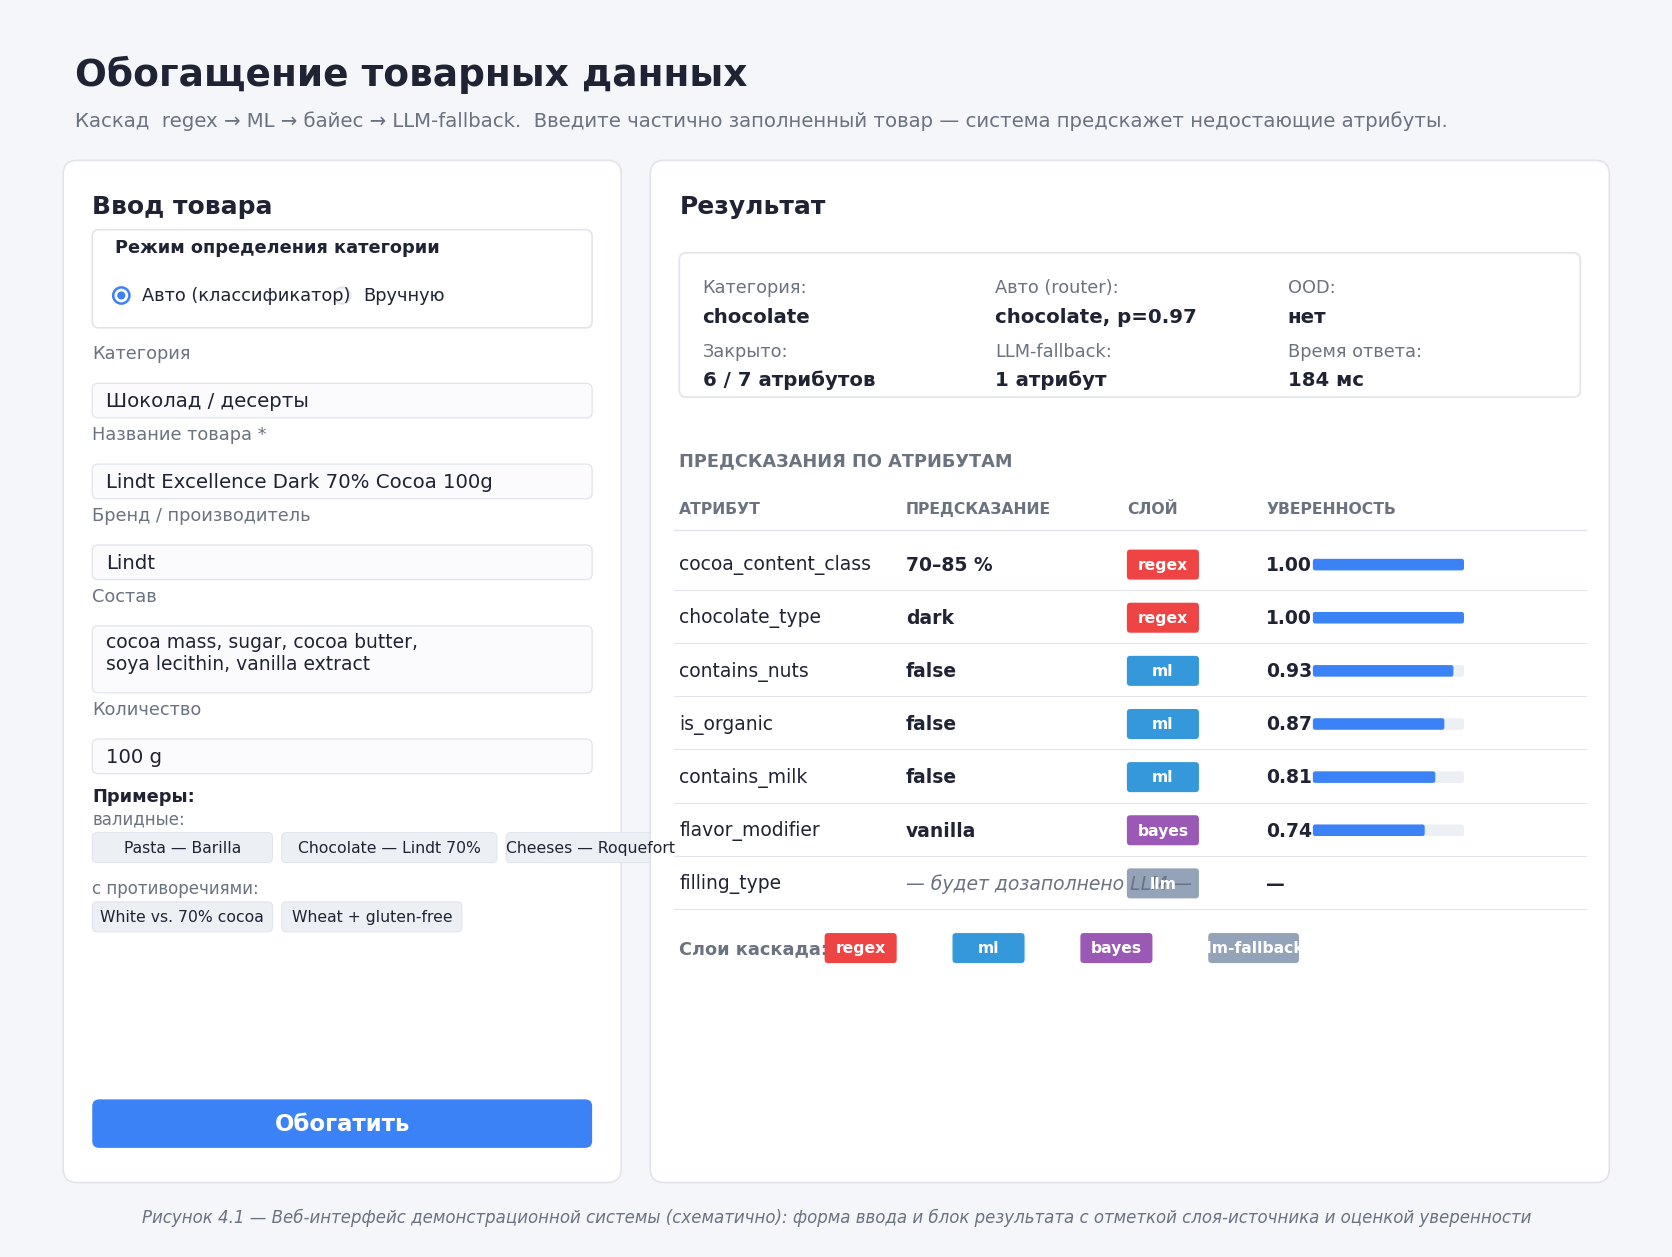
\includegraphics[width=\textwidth]{fig_4_1_demo_ui.png}
  \caption{Веб-интерфейс демонстрационной системы (схематично): форма ввода партнёр-доступных полей и блок результата с отметкой слоя-источника и оценкой уверенности на каждый атрибут}
  \label{fig:fig_4_1_demo_ui}
\end{figure}

Отметка слоя-источника даёт основание для доверия к предсказанию: слой 1 и слой 4 детерминированы либо объяснимы, для слоя 2 и слоя 3 показателем служит уверенность. Приём введён (см. 1.3) для компенсации ограниченной интерпретируемости слоёв 2/3 на уровне отдельного товара.

\subsubsection{Системный аналитик}

Аналитик настраивает каскад через две точки. Первая — словари порогов \texttt{models/\{category\}\_thresholds.pkl}: контролируют компромисс «точность ↔ покрытие» поатрибутно, изменение не требует переобучения, применяется при следующем старте сервиса (типовой инструмент тонкой настройки при изменении требований к качеству). Вторая — REST API: \texttt{GET /api/categories} (состав атрибутов), \texttt{GET /health} (агрегированное состояние) для интеграции с мониторингом.

\subsubsection{Инженер машинного обучения}

Инженер работает с модулями \texttt{src/} через \texttt{python -m src.<module>} и ноутбуком \texttt{notebooks/00\_thesis\_main.ipynb}. Цикл переобучения устроен так, что выпуск новой версии моделей не требует перекомпиляции каскада: файлы в \texttt{models/} переписываются, ML-сервис при старте загружает обновлённые артефакты. Последовательность команд цикла переобучения:

\begin{verbatim}
source .venv/bin/activate
python -m src.data.label_silver --category pasta_stratified
OMP_NUM_THREADS=1 python -m src.pipeline.ml.train    --category pasta_stratified
OMP_NUM_THREADS=1 python -m src.pipeline.bayes.train --category pasta_stratified
OMP_NUM_THREADS=1 python -m src.eval.run_experiments  --category pasta_stratified
OMP_NUM_THREADS=1 python -m src.eval.run_diagnostics
\end{verbatim}

Цикл запускается еженедельно или ежемесячно (зависит от темпа поступления товаров) и занимает десятки минут на категорию без специализированных ресурсов.

\subsection{Сценарии применения и порядок внедрения}

\subsubsection{Встраивание в бизнес-процесс магазина}

Каскад занимает место промежуточного сервиса в маршруте товара от поставщика до витрины — вторая позиция четырёхзвенной цепочки 1.1, где сосредоточено узкое место. Внедрение не требует перестройки соседних звеньев: ETL партнёрских фидов и PIM работают как раньше, изменяется лишь содержимое «процедуры обогащения». Цепочка обработки:

\begin{verbatim}
Партнёрский фид (CSV/JSON/XML) → ETL магазина (нормализация полей)
  → HTTP /api/enrich — каскад (regex → ML → Bayes → LLM-fallback)
  → Контент-менеджер (выборочная проверка случаев слоя 4)
  → PIM (финальная карточка) → Витрина и поисковый индекс
\end{verbatim}

Основной экономический эффект — перенос ручного труда из режима «закрывать каждое поле» в режим «проверять остаток после каскада». По 3.3.2 каскад покрывает 96,7 \% ячеек без LLM, оставшиеся 3,3 \% уходят в запасной слой; сквозная точность 92,8 \% в конфигурации «каскад + gemini-flash».

\subsubsection{Сценарий холодного старта новой категории}

Для новой категории каскад деградирует до двух слоёв (слой 1 на общих шаблонах + слой 4) — рабочий, но неоптимальный режим: точность слоя 4 на нутриент-производных атрибутах ниже, чем у обученного слоя 2 (4.3.3), стоимость выше. По мере накопления сотен размеченных товаров подключается слой 2; при появлении устойчивых распределений по брендам — слой 3.

Электроника использована как контрольный домен холодного старта (эталон — поля технических характеристик PhoneDB \cite{ref_45} без слабого надзора). Полноценная аудит-оценка по протоколу 3.3 вынесена в раздел «Перспективы развития темы» заключения.

\subsubsection{Сценарий многоязычного каталога}

\texttt{paraphrase-multilingual-MiniLM-L12-v2} обеспечивает единое векторное пространство для пяти доминирующих в OFF европейских языков, что устраняет необходимость отдельных моделей под каждый язык. Устойчивость по языкам подтверждена в 3.3.7.1: разброс между лучшим и худшим сегментом — 2,9 п. п. Каскад применим в международных площадках без удвоения затрат на поддержку.

\subsubsection{Сценарий обогащения нутриентно-производных полей}

Атрибуты, восходящие к числовым нутриентам, требуют точного числового ответа. Одиночный вызов LLM малопригоден из-за высокой частоты ошибок на числах (1.2). В каскаде такие атрибуты закрываются комбинацией слоя 1 (числовые шаблоны) и слоя 2 (классификация дискретных классов после бакетирования нутриентов). USDA Branded Foods используется на этапе обучения для сверки эталона яруса 0 (3.2.5); расширение каскада детерминированным USDA-слоем в режиме вывода — в разделе «Перспективы развития темы» заключения.

\subsubsection{Применимость в смежных доменах}

Архитектура не привязана к пищевому домену: правила слоя 1 переписываются для новой категории, обучение слоёв 2/3 — стандартная процедура. Репликация на электронике (схема атрибутов, серебро из PhoneDB, демонстрация холодного старта; подробности в разделе «Перспективы развития темы» заключения) подтверждает переносимость. Формальная аудит-оценка вынесена в перспективы развития.

\subsection{Что позволяет использование разработки (характеристика достигнутых результатов)}

Использование системы даёт пять измеримых эффектов в формате «повышено / ускорено / сокращено» со ссылками на 3.

\subsubsection{Повышено: качество автоматического обогащения каталога}

Сквозная точность на 4350 ячейках без пересечения брендов — 92,8 \% в конфигурации «каскад + gemini-flash» (3.3.2; \texttt{grand\_acc\_summary\_after\_fix.parquet}). 95 \%-й интервал Вильсона: [92,0; 93,6] для «каскад + gemini-flash» и [89,6; 91,4] для «только каскад» (90,5 \%). Поатрибутный разрез по категориям приведён в таблице 4.2 (источник: \texttt{headline\_v3e\_after\_fix.parquet}).

\begin{xltabular}{\textwidth}{|X|X|X|X|}
\caption{Сквозная точность каскада по категориям (модель gemini-flash, 4350 ячеек без пересечения брендов)} \\ \hline
    Категория & Только каскад & Каскад + gemini-flash & Прирост \\ \hline
\endfirsthead
\multicolumn{4}{l}{\textit{Продолжение таблицы}} \\ \hline
    Категория & Только каскад & Каскад + gemini-flash & Прирост \\ \hline
\endhead
    Паста & 93,3 \% & 95,8 \% & +2,5 п. п. \\ \hline
    Шоколад & 87,4 \% & 90,1 \% & +2,7 п. п. \\ \hline
    Сыры & 90,4 \% & 92,2 \% & +1,8 п. п. \\ \hline
    Взвешенное среднее & 90,5 \% & 92,8 \% & +2,3 п. п. \\ \hline
\end{xltabular}

\textit{Примечание. Источник: \texttt{headline\_v3e\_after\_fix.parquet}.}

Сыры и шоколад получают наибольший выигрыш от запасного слоя на оставшихся ≈3 \% сложных ячеек. На пасте, где правила слоя 1 покрывают значительную долю, прирост от слоя 4 минимален.

Сравнение с альтернативами: прямой Claude Sonnet 4.5 даёт 83,8 \% (на 9,0 п. п. ниже системы); прямой gpt-oss-120b — 69,3 \% (на 23,0 п. п. ниже каскада с этой же моделью в роли слоя 4 — 92,3 \%). Превосходство объясняется наличием специализированных слоёв: Слой 2 обучен на нутриент-производных атрибутах (Nutri-Score, класс белка, класс жирности), которые LLM не вычисляет точно из текста без доступа к числам.

\subsubsection{Сокращено: стоимость обработки в 720 раз относительно эталонной LLM-модели}

Стоимость обработки одного товара через каскад + gemini-flash составляет ≈0,14 \% стоимости прямого Sonnet 4.5 (сокращение в 720 раз при превышении точности на 9,0 п. п.; матрица — 3.3.2). Экономия — за счёт обработки полей в порядке возрастания стоимости: Слой 1 (бесплатно) → Слой 2 (миллисекунды на CPU) → Слой 3 (локальный вывод) → Слой 4 только при отказе предыдущих. По 3.3 LLM вызывается на 3,3 \% ячеек, а не на 100 \%. Стоимость пяти каскадных конфигураций относительно опорной «все ячейки — Sonnet 4.5» приведена в таблице 4.3 (источник: \texttt{grand\_acc\_summary\_after\_fix.parquet}).

\begin{xltabular}{\textwidth}{|X|X|X|}
\caption{Стоимость обработки одного товара относительно опорной конфигурации all-sonnet} \\ \hline
    Конфигурация & Стоимость относительно опорной & Снижение стоимости \\ \hline
\endfirsthead
\multicolumn{3}{l}{\textit{Продолжение таблицы}} \\ \hline
    Конфигурация & Стоимость относительно опорной & Снижение стоимости \\ \hline
\endhead
    Каскад + gemini-flash & 0,0014 & в 720 раз \\ \hline
    Каскад + gpt-4o & 0,024 & в 42 раза \\ \hline
    Каскад + Claude Sonnet 4.5 & 0,033 & в 30 раз \\ \hline
    Каскад + gpt-oss-120b (открытая модель) & 0,0010 & в 1007 раз \\ \hline
\end{xltabular}

\textit{Примечание. Источник: \texttt{grand\_acc\_summary\_after\_fix.parquet}.}

При сценарии 100 000 товаров/месяц экономия составляет порядки величины относительно прямого вызова LLM.

\subsubsection{Обеспечена: возможность развёртывания на собственных мощностях с открытой моделью}

Система поддерживает gpt-oss-120b в роли слоя 4 — полностью локальное развёртывание без отправки партнёрских данных вовне. Сводно (3.3.2): сквозная точность каскад + gpt-oss-120b — 92,3 \%; прямой gpt-oss-120b — 69,3 \%; прирост от каскадной архитектуры — +23,0 п. п. (слой 2 закрывает атрибуты, на которых малая модель проигрывает); стоимость сценария ≈в 30 раз ниже прямого использования за счёт сокращения LLM-вызовов до 3,3 \% ячеек. При потере 0,5 п. п. точности относительно gemini-flash обеспечивается независимость от внешних API — критично для корпоративных сценариев с требованиями локального хранения данных.

\subsubsection{Сокращён: ручной труд оператора каталога}

В исходном процессе (1.1) оператор проверяет каждый атрибут — 100 \% ручной работы. Система переводит труд в режим выборочной верификации: 96,7 \% ячеек закрываются дешёвыми слоями автоматически; 3,3 \% уходят в слой 4 и получают предсказание (часть требует верификации, обычно — помеченные байесовский валидатором); совокупная доля ручной верификации — 3–7 \% в зависимости от порога валидатора (3.3.4). Ручная нагрузка сокращается в 10–20 раз; контроль качества сохраняется через отметку слоя-источника и доверительные индикаторы.

\subsubsection{Повышена: устойчивость каталога к смещению по брендам}

Тестирование без пересечения брендов (3.2.4) подтверждает обобщение на бренды, не встречавшиеся в обучении: на 4350 ячейках средняя точность 92,8 \% с интервалом Вильсона [92,0; 93,6]. Дополнительно k-NN-абляция (3.3.7.3) показывает: точность не падает на удалённых от обучения товарах, а монотонно растёт от Q1 (82,7 \%) до Q4 (91,6 \%).

\subsubsection{Резюмирующая таблица «повышено / ускорено / сокращено»}

Сводный эффект разработки на семи показателях приведён в таблице 4.4 (источники: \texttt{grand\_acc\_summary\_after\_fix.parquet}, \texttt{headline\_v3e\_after\_fix.parquet}).

\begin{xltabular}{\textwidth}{|X|X|X|X|}
\caption{Сводный эффект разработки на ключевых показателях системы (повышено / сокращено / обеспечено)} \\ \hline
    Показатель & До разработки & После & Эффект \\ \hline
\endfirsthead
\multicolumn{4}{l}{\textit{Продолжение таблицы}} \\ \hline
    Показатель & До разработки & После & Эффект \\ \hline
\endhead
    Сквозная точность системы & 83,8 \% (опорная конфигурация all-sonnet) & 92,8 \% (каскад + gemini-flash) & повышена на 9,0 п. п. \\ \hline
    Относительная стоимость обработки & 1,000 (опорная конфигурация all-sonnet) & 0,0014 (каскад + gemini-flash) & сокращена в 720 раз \\ \hline
    Доля обращений к LLM & 100 \% & 3,3 \% & сокращена в 30 раз \\ \hline
    Ручная верификация оператором & ~100 \% ячеек & ~5–10 \% ячеек & сокращена в 10–20 раз \\ \hline
    Точность на открытой модели & 69,3 \% (одиночный вызов gpt-oss-120b) & 92,3 \% (каскад + gpt-oss-120b) & повышена на 23,0 п. п. \\ \hline
    Поддержка многоязычности & отдельные модели на каждый язык либо предварительный перевод & 5 рабочих языков в едином векторном пространстве SBERT & обеспечена без дополнительных моделей \\ \hline
    Независимость от поставщика LLM & один интегрированный провайдер & поддержка пяти моделей с сопоставимой точностью & обеспечена взаимозаменяемость \\ \hline
\end{xltabular}

\textit{Примечание. Источники: \texttt{grand\_acc\_summary\_after\_fix.parquet}, \texttt{headline\_v3e\_after\_fix.parquet}.}

Значения столбцов «До» и «После» получены на тестовой выборке без пересечения брендов главы 3 и подтверждены артефактами \texttt{grand\_acc\_summary\_after\_fix.parquet} и \texttt{headline\_v3e\_after\_fix.parquet}.

\subsection{Выводы по главе 4}

\begin{enumerate}[arabic]
    \item Система допускает три сценария по выбору слоя 4: бюджетный коммерческий (gemini-flash) — наилучший баланс точности и стоимости; премиум-коммерческий (Sonnet 4.5, GPT-4o) — близкая точность при большей стоимости; локальное развёртывание с gpt-oss-120b — независимость от внешних API при потере 0,5 п. п. точности.
    \item Целевая аудитория — три роли: контент-менеджер (выборочная верификация через веб-интерфейс), системный аналитик (пороги через конфигурации и REST API), инженер ML (переобучение по мере поступления данных).
    \item Совокупный эффект: сокращение стоимости в 720 раз относительно прямого вызова LLM и ручной нагрузки в 10–20 раз при точности 92,8 \% на выборке без пересечения брендов с интервалом Вильсона [92,0; 93,6].
\end{enumerate}
         % Глава 4

    \conclusion

В ходе работы разработана гибридная каскадная система автоматизированного обогащения товарных данных для интернет-магазина. Система реализована в виде программного комплекса с демонстрационным стендом, проверена на выборке без пересечения брендов и удовлетворяет шести функциональным, пяти нефункциональным и четырём архитектурным требованиям ТЗ.

Достигнутые показатели превосходят целевые ориентиры ТЗ (≥ 85 \% точности, ≥ 2,5× сокращения стоимости): сквозная точность 92,8 \%, стоимость сокращена в 720 раз относительно прямого вызова коммерческой LLM. Каскад без запасного слоя покрывает 96,7 \% ячеек со средней точностью 90,5 \%; в LLM направляется лишь 3,3 \% сложных ячеек.

\subsection*{Сводные выводы по главам}

\textbf{Глава 1} систематизирует литературу и обосновывает противоречие. PIM-системы (Akeneo \cite{ref_5}, Pimcore \cite{ref_6}, Salsify \cite{ref_7}) ориентированы на хранение и распределение, а появляющиеся модули автоматического обогащения — обёртки над одной LLM, не отвечающие требованиям больших каталогов. Академические подходы разделены: специализированные системы извлечения признаков (TXtract \cite{ref_23}, MAVE \cite{ref_24}, OpenTag \cite{ref_25}) обеспечивают качество без учёта экономики; каскады LLM (FrugalGPT \cite{ref_9}, AutoMix \cite{ref_10}, Hybrid LLM \cite{ref_11}, RouterBench \cite{ref_12}) дают инструменты управления стоимостью, но не интегрируют классическое ML. Из противоречия выведена гипотеза о каскаде разнородных слоёв и ТЗ.

\textbf{Глава 2.} Задача формализована как поатрибутное предсказание со схемой, допускающей явный отказ. Логика — каскад из пяти слоёв с последовательной фильтрацией: предсказание Слой 2 принимается только при одновременном выполнении $P_{\text{ML}} \geq \tau_k$ и $P_B \geq \theta_k$ — формализация ансамблевой оценки уверенности как AND-условия. Архитектурный выбор каждой компоненты (SBERT, XGBoost, pgmpy, Go-шлюз + Python-ML, открытая gpt-oss-120b) обоснован эксплуатационно, методологически и стратегически.

\textbf{Глава 3.} Каскад реализован как трёхкомпонентный комплекс (Go-шлюз, Python/FastAPI ML-сервис, статический веб-интерфейс); состав — 24 поатрибутных XGBoost (8/7/9 для pasta/chocolate/cheeses), три байесовские сети и Слой 0. На 4350 ячейках без пересечения брендов сквозная точность каскад + Gemini 2.5 Flash — 92,8 \%, на 9,0 п. п. выше прямого Sonnet 4.5 при стоимости в 720 раз ниже; в сценарии локального развёртывания каскад + gpt-oss-120b — 92,3 \% (на 23,0 п. п. выше самостоятельного использования). Слой 1 закрывает 18–23 \% pasta/chocolate с точностью 87–90 \% и 3 \% cheeses со 100 \% precision; Слой 2 — 72–94 \% покрытия при 93,5–98,6 \% точности; байесовский валидатор работает селективно на chocolate/contains\_nuts; LLM добавляет 2,3 п. п. при 3,3 \% обращений. Зафиксированная до получения результатов H1 о превосходстве обучаемого маршрутизатора отклонена. Цикл «аудит — правки — переобучение — измерение» воспроизведён 3/3 с приростом +18,2, +16,3 и +14,4 п. п.

\textbf{Глава 4} переводит результаты в плоскость применения: три сценария по выбору слоя 4 (gemini-flash, Sonnet/GPT-4o, локально развёрнутая gpt-oss-120b); три ролевые модели (контент-менеджер, системный аналитик, инженер ML). Сводный эффект — сокращение стоимости в 720 раз и ручной нагрузки в 10–20 раз при точности 92,8 \% с интервалом Вильсона [92,0; 93,6].

\subsection*{Закрытие формулировок утверждённой темы}

Утверждённая тема работы содержит восемь содержательных формулировок. Каждой из них в работе соответствует конкретный раздел, а также архитектурный или экспериментальный компонент разработки. Соответствие представлено в таблице 5.1.

\begin{xltabular}{\textwidth}{|X|X|X|}
\caption{Соответствие формулировок утверждённой темы и разделов работы} \\ \hline
    Формулировка из обоснования актуальности темы & Реализация в работе & Раздел \\ \hline
\endfirsthead
\multicolumn{3}{l}{\textit{Продолжение таблицы}} \\ \hline
    Формулировка из обоснования актуальности темы & Реализация в работе & Раздел \\ \hline
\endhead
    Гибридная каскадная система & Пятислойная архитектура каскада (Слой 0 + четыре содержательных слоя) & 2.2, 3.1 \\ \hline
    Семантические возможности генеративных моделей & Запасной слой 4 на основе большой языковой модели & 3.1.1 \\ \hline
    Предсказательная сила классического машинного обучения & Слой 2 — поатрибутные классификаторы XGBoost на многоязычных векторных представлениях SBERT & 3.1.1 \\ \hline
    Ансамблевая оценка уверенности моделей & Многоуровневая фильтрация по уверенности как последовательное конъюнктивное условие на калиброванные пороги слоёв & 2.1 \\ \hline
    Отбраковка фактических ошибок до их попадания в каталог & Слой 3 — байесовский валидатор плотностей пар «бренд × значение» & 3.1.1, 3.3.4 \\ \hline
    Скрытые статистические закономерности каталога & Направленный ациклический граф атрибутов, обучаемый алгоритмом Hill Climb с критерием BIC & 3.1.1 \\ \hline
    Разнородные источники данных (мультимодальные и многоканальные) & OCR-извлечение из изображений Open Food Facts и эмбеддинги CLIP на этапе обучения; нечёткое сопоставление с базой USDA Branded Foods для производных атрибутов & 3.2.5 \\ \hline
    Интернет-магазин (партнёр — каталог — витрина) & Демонстрационный программный комплекс с REST-интерфейсом обработки партнёрского ввода и руководством пользователя & 1.1, 3.1.2, 4.1 \\ \hline
\end{xltabular}

Таким образом, все восемь содержательных формулировок утверждённой темы имеют прямое отображение в разработанной системе и подтверждены экспериментально либо архитектурно. Наиболее нагруженные формулировки — отбраковка фактических ошибок и использование скрытых статистических закономерностей каталога — закрыты слоем байесовского валидатора. Для него в работе пересмотрена роль: вместо самостоятельного классификатора сеть используется как валидатор плотностей.

\subsection*{Научная новизна}

Научная новизна работы складывается из трёх содержательных пунктов.

\begin{enumerate}[arabic]
    \item Доминирование каскадной архитектуры по Парето над всеми безусловными конфигурациями большой языковой модели на задаче обогащения товарных атрибутов. Одновременно достигается превышение точности на 9,0 процентных пункта и снижение стоимости в 720 раз по сравнению с прямым обращением к Claude Sonnet 4.5. Результат подтверждён на проверочной выборке без пересечения брендов из 4350 ячеек и воспроизведён на пяти различных моделях запасного слоя. Это означает, что эффект сохраняется при смене поставщика генеративной модели.
    \item Сценарий развёртывания на собственных мощностях с открытой большой языковой моделью. Каскад с открытой моделью gpt-oss-120b достигает 92,3 \% сквозной точности — на 23,0 процентных пункта выше, чем самостоятельное применение той же модели. Результат демонстрирует способность каскадной композиции компенсировать слабость малых открытых моделей через специализированные слои. Кроме того, он формирует методологическую основу для локального развёртывания системы без передачи партнёрских данных во внешние коммерческие сервисы.
    \item Зафиксированный до получения результатов отрицательный результат для обучаемого стоимостно-чувствительного маршрутизатора и кросс-доменная репликация цикла «аудит — исправления — переобучение — измерение». Гипотеза о превосходстве обучаемого XGBoost-маршрутизатора над статическим правилом отклонена на трёх бюджетах с поправкой Бонферрони. Этот результат согласуется с выводами бенчмарка RouterBench \cite{ref_12}. Цикл аудита эталонной разметки воспроизведён на трёх категориях из трёх с количественно измеримым приростом сквозной точности.
\end{enumerate}

\subsection*{Ограничения работы}

Результаты ограничены рядом обстоятельств, добросовестно фиксируемых для формирования перспектив. Во-первых, область определения ограничена тремя категориями пищевой продукции; переносимость на другие домены не валидирована. Во-вторых, эталон построен сочетанием слабого надзора и согласия трёх LLM со слепой проверкой Opus 4 — аудит-эталон второго уровня, ручная экспертная разметка не выполнялась. В-третьих, мультимодальные сигналы OCR и CLIP используются только на обучении; в выводе работают только текстовые поля. В-четвёртых, проверка ограничена пятью европейскими языками, устойчивость к иным письменностям не валидирована. В-пятых, предварительная регистрация ограничена H1; показатели 3.3.2 — post-hoc анализ.

Селективный характер байесовского валидатора (значимый прирост точности отбраковки на 3 парах из 22) ограничением не считается, а признаётся архитектурным свойством. В финальной конфигурации валидатор включён точечно на chocolate/contains\_nuts, где даёт +6,6 п. п. точности при росте расходов на 5,3 п. п. (3.3.4). Принцип «изменение роли компонента вместо его удаления» сформулирован в 3.1.1 и 3.3.4 как самостоятельный методологический вывод.

\subsection*{Перспективы развития темы}

Полученные результаты и зафиксированные ограничения определяют ряд перспективных направлений развития темы.

\begin{enumerate}[arabic]
    \item Расширение области определения до шести категорий — напитки, зерновые завтраки и косметика. Для этих категорий подготовлены схемы атрибутов и серебряная разметка в файлах \texttt{beverages\_stratified\_silver\_standard.parquet}, \texttt{cereals\_stratified\_silver\_standard.parquet} и \texttt{cosmetics\_stratified\_silver\_standard.parquet}. Основной блокер расширения — построение аудит-эталона уровня итоговой эталонной разметки v2 для каждой категории и обучение поатрибутных классификаторов Слой 2. Методология аудита и переобучения предположительно переносится на новые категории без принципиальных изменений.
    \item Регулярная переаттестация изотонической калибровки на следующих итерациях эталонной разметки. Эффект схемы перекрёстной калибровки экспериментально проверен и реализован в коде системы (3.3.3.3, флаг \texttt{--calibration-method isotonic} в \texttt{src/pipeline/ml/train.py}). Средняя ECE снижается с 0,070 до 0,043, что даёт улучшение на 2,78 п. п. в среднем и прирост на 18 из 22 атрибутов. Перспектива заключается в переаттестации после расширения эталонной разметки до большего числа атрибутов и категорий. Также целесообразно добавить регрессионный тест на ухудшение ECE более чем на 0,01 как условие принятия следующего цикла переобучения.
    \item Введение мультимодального вывода в производственный режим — расширение прикладного интерфейса на приём изображений и добавление OCR/CLIP в реальном времени. Такой шаг требует пересмотра контракта взаимодействия с партнёром.
    \item Запуск пилотного активного обучения на ячейках расхождения каскада и запасного слоя \cite{ref_46, ref_39}. Логика построения очереди ячеек, где предсказание слоя 2 расходится с ответом запасного слоя, реализована в \texttt{src/experiments/active\_learning\_pilot.py}. Скрипт выполняет выборку 5 000 кодов на категорию, отбор 150 неуверенных и 150 случайных контрольных, а также повторное обучение с замером прироста на отложенной выборке. Перспектива заключается в проведении пилота в полном объёме на трёх категориях и в измерении прироста точности слоя 2 относительно случайной разметки той же стоимости.
    \item Использование базы USDA Branded Foods и аналогов как структурированного второго источника для производных атрибутов с систематизацией политики приоритетов между партнёрским вводом и вторичными каталогами.
    \item Локализация на русский язык и российские каталоги — разработка русскоязычных регулярных выражений слоя 1 и дообучение слоя 2 на каталогах российских ритейлеров. Поскольку SBERT поддерживает русский в едином векторном пространстве, трудоёмкость ограничена слоями 1–2.
    \item Перенос архитектуры в непродовольственные домены, начиная с электроники. Для смартфонов из каталога PhoneDB подготовлены схема атрибутов, скрипт построения серебряного стандарта и демонстрация холодного старта. Полноценное измерение точности требует построения аудит-эталона уровня итоговой эталонной разметки v2 и оценки без пересечения брендов. Электроника сохранена как контрольный домен проверки переносимости и в основную таблицу 3.3 не входит.
\end{enumerate}

Таким образом, разработанная гибридная каскадная система демонстрирует возможность одновременно достигать высокой точности и низкой стоимости обогащения товарных каталогов. Этот результат обеспечивается за счёт стратифицированного распределения нагрузки между разнородными по природе слоями обработки. Полученные результаты подтверждают выдвинутую в первой главе работы архитектурную гипотезу о каскадной композиции и закрывают все восемь содержательных формулировок утверждённой темы.
    % ЗАКЛЮЧЕНИЕ

    \printbibliography                 % Список использованных источников

    \appendix
    \appendixsection{Электронные материалы}

На рисунке~\ref{fig:qr-git} приведён QR-код со ссылкой на репозиторий с
исходным кодом, ноутбуком §3.3 в исполняемом виде, демонстрационным
программным комплексом и текстом настоящей работы.

\begin{figure}[h]
    \centering
    
\includegraphics[width=5cm]{qr-git.pdf}
    \caption{QR-код на репозиторий проекта}
    \label{fig:qr-git}
\end{figure}
  % ПРИЛОЖЕНИЕ А — Электронные материалы
\end{document}
